\documentclass[12pt, twoside, openright]{report} %fuente a 12pt, formato doble pagina y chapter a la derecha
\raggedbottom % No ajustar el contenido con un salto de pagina

% MÁRGENES: 2,5 cm sup. e inf.; 3 cm izdo. y dcho.
\usepackage[
a4paper,
vmargin=2.5cm,
hmargin=3cm
]{geometry}

% INTERLINEADO: Estrecho (6 ptos./interlineado 1,15) o Moderado (6 ptos./interlineado 1,5)
\renewcommand{\baselinestretch}{1.15}
\parskip=6pt

% DEFINICIÓN DE COLORES para portada y listados de código
\usepackage[table]{xcolor}
\definecolor{azulUC3M}{RGB}{0,0,102}
\definecolor{gray97}{gray}{.97}
\definecolor{gray75}{gray}{.75}
\definecolor{gray45}{gray}{.45}

% Soporte para GENERAR PDF/A
\usepackage[a-1b]{pdfx}

% ENLACES
\usepackage{hyperref}
\hypersetup{colorlinks=true,
	linkcolor=black, % enlaces a partes del documento (p.e. índice) en color negro
	urlcolor=blue} % enlaces a recursos fuera del documento en azul

% Añadir pdfs como partes del documento
\usepackage{pdfpages}

% Quitar la indentación de principio de los parrafos
\setlength{\parindent}{0em}

% EXPRESIONES MATEMATICAS
\usepackage{amsmath,amssymb,amsfonts,amsthm}

\usepackage{txfonts} 
\usepackage[T1]{fontenc}
\usepackage[utf8]{inputenc}

% Insertar graficas y fotos
\usepackage{tikz}
\usepackage{pgfplots}

\usepackage[spanish, es-tabla]{babel} 
\usepackage[babel, spanish=spanish]{csquotes}
\AtBeginEnvironment{quote}{\small}

% diseño de PIE DE PÁGINA
\usepackage{fancyhdr}
\pagestyle{fancy}
\fancyhf{}
\renewcommand{\headrulewidth}{0pt}
\fancyfoot[LE,RO]{\thepage}
\fancypagestyle{plain}{\pagestyle{fancy}}

% DISEÑO DE LOS TÍTULOS de las partes del trabajo (capítulos y epígrafes o subcapítulos)
\usepackage{titlesec}
\usepackage{titletoc}
\titleformat{\chapter}[block]
{\large\bfseries\filcenter}
{\thechapter.}
{5pt}
{\MakeUppercase}
{}
\titlespacing{\chapter}{0pt}{0pt}{*3}
\titlecontents{chapter}
[0pt]                                               
{}
{\contentsmargin{0pt}\thecontentslabel.\enspace\uppercase}
{\contentsmargin{0pt}\uppercase}                        
{\titlerule*[.7pc]{.}\contentspage}                 

\titleformat{\section}
{\bfseries}
{\thesection.}
{5pt}
{}
\titlecontents{section}
[5pt]                                               
{}
{\contentsmargin{0pt}\thecontentslabel.\enspace}
{\contentsmargin{0pt}}
{\titlerule*[.7pc]{.}\contentspage}

\titleformat{\subsection}
{\normalsize\bfseries}
{\thesubsection.}
{5pt}
{}
\titlecontents{subsection}
[10pt]                                               
{}
{\contentsmargin{0pt}                          
	\thecontentslabel.\enspace}
{\contentsmargin{0pt}}                        
{\titlerule*[.7pc]{.}\contentspage}  


% DISEÑO DE TABLAS.
\usepackage{multirow} % permite combinar celdas 
\usepackage{caption} % para personalizar el título de tablas y figuras
\usepackage{floatrow} % utilizamos este paquete y sus macros \ttabbox y \ffigbox para alinear los nombres de tablas y figuras de acuerdo con el estilo definido. Para su uso ver archivo de ejemplo 
\usepackage{array} % con este paquete podemos definir en la siguiente línea un nuevo tipo de columna para tablas: ancho personalizado y contenido centrado
\newcolumntype{P}[1]{>{\centering\arraybackslash}p{#1}}
\DeclareCaptionFormat{upper}{#1#2\uppercase{#3}\par}

% Diseño de tabla para ingeniería
\captionsetup[table]{
	format=hang,
	name=Tabla,
	justification=centering,
	labelsep=colon,
	width=.75\linewidth,
	labelfont=small,
	font=small,
}

% DISEÑO DE FIGURAS.
\usepackage{graphicx}
\graphicspath{{img/}} %ruta a la carpeta de imágenes

% Diseño de figuras para ingeniería
\captionsetup[figure]{
	format=hang,
	name=Fig.,
	singlelinecheck=off,
	labelsep=colon,
	labelfont=small,
	font=small		
}

% NOTAS A PIE DE PÁGINA
\usepackage{chngcntr} %para numeración continua de las notas al pie
\counterwithout{footnote}{chapter}

% LISTADOS DE CÓDIGO
% soporte y estilo para listados de código. Más información en https://es.wikibooks.org/wiki/Manual_de_LaTeX/Listados_de_código/Listados_con_listings
\usepackage{listings}

% definimos un estilo de listings
\lstdefinestyle{estilo}{ frame=Ltb,
	framerule=0pt,
	aboveskip=0.5cm,
	framextopmargin=3pt,
	framexbottommargin=3pt,
	framexleftmargin=0.4cm,
	framesep=0pt,
	rulesep=.4pt,
	backgroundcolor=\color{gray97},
	rulesepcolor=\color{black},
	%
	basicstyle=\ttfamily\footnotesize,
	keywordstyle=\bfseries,
	stringstyle=\ttfamily,
	showstringspaces = false,
	commentstyle=\color{gray45},     
	%
	numbers=left,
	numbersep=15pt,
	numberstyle=\tiny,
	numberfirstline = false,
	breaklines=true,
	xleftmargin=\parindent
}

\captionsetup[lstlisting]{font=small, labelsep=period}
% fijamos el estilo a utilizar 
\lstset{style=estilo}
\renewcommand{\lstlistingname}{\uppercase{Código}}

\pgfplotsset{compat=1.17} 
%-------------
%	DOCUMENTO
%-------------

\begin{document}
\pagenumbering{roman} % Se utilizan cifras romanas en la numeración de las páginas previas al cuerpo del trabajo
	
%----------
%	PORTADA
%----------	
\begin{titlepage}
	\begin{sffamily}
	\color{azulUC3M}
	\begin{center}
		\begin{figure}[H] %incluimos el logotipo de la Universidad
			\makebox[\textwidth][c]{
\includegraphics[width=16cm]{Portada_Logo.png}}
		\end{figure}
		\vspace{2.5cm}
		\begin{Large}
			Grado en Ingeniería Informática\\			
			2020-2021\\
			\vspace{2cm}		
			\textsl{Apuntes}\\
			\bigskip
		\end{Large}
		 	{\Huge Heurística y Optimización}\\
		 	\vspace*{0.5cm}
	 		\rule{10.5cm}{0.1mm}\\
			\vspace*{0.9cm}
			{\LARGE Jorge Rodríguez Fraile\footnote{\href{mailto:100405951@alumnos.uc3m.es}{Universidad: 100405951@alumnos.uc3m.es}  |  \href{mailto:jrf1616@gmail.com}{Personal: jrf1616@gmail.com}}}\\ 
			\vspace*{1cm}
	\end{center}
	\vfill
	\color{black}
		
\includegraphics[width=4.2cm]{img/creativecommons.png}\\
		Esta obra se encuentra sujeta a la licencia Creative Commons\\ \textbf{Reconocimiento - No Comercial - Sin Obra Derivada}
	\end{sffamily}
\end{titlepage}

%----------
%	ÍNDICES
%----------	

%--
% Índice general
%-
\tableofcontents
\thispagestyle{fancy}

%--
% Índice de figuras. Si no se incluyen, comenta las líneas siguientes
%-
\listoffigures
\thispagestyle{fancy}

%----------
%	TRABAJO
%----------	

\pagenumbering{arabic} % numeración con múmeros arábigos para el resto de la publicación	


%----------
%	COMENZAR A ESCRIBIR AQUI
%----------	

\chapter{Información}
\section{Profesores}
\begin{quote}
Magistral: Carlos Linares López 

Reducido: Francisco Javier García Polo
  \end{quote}

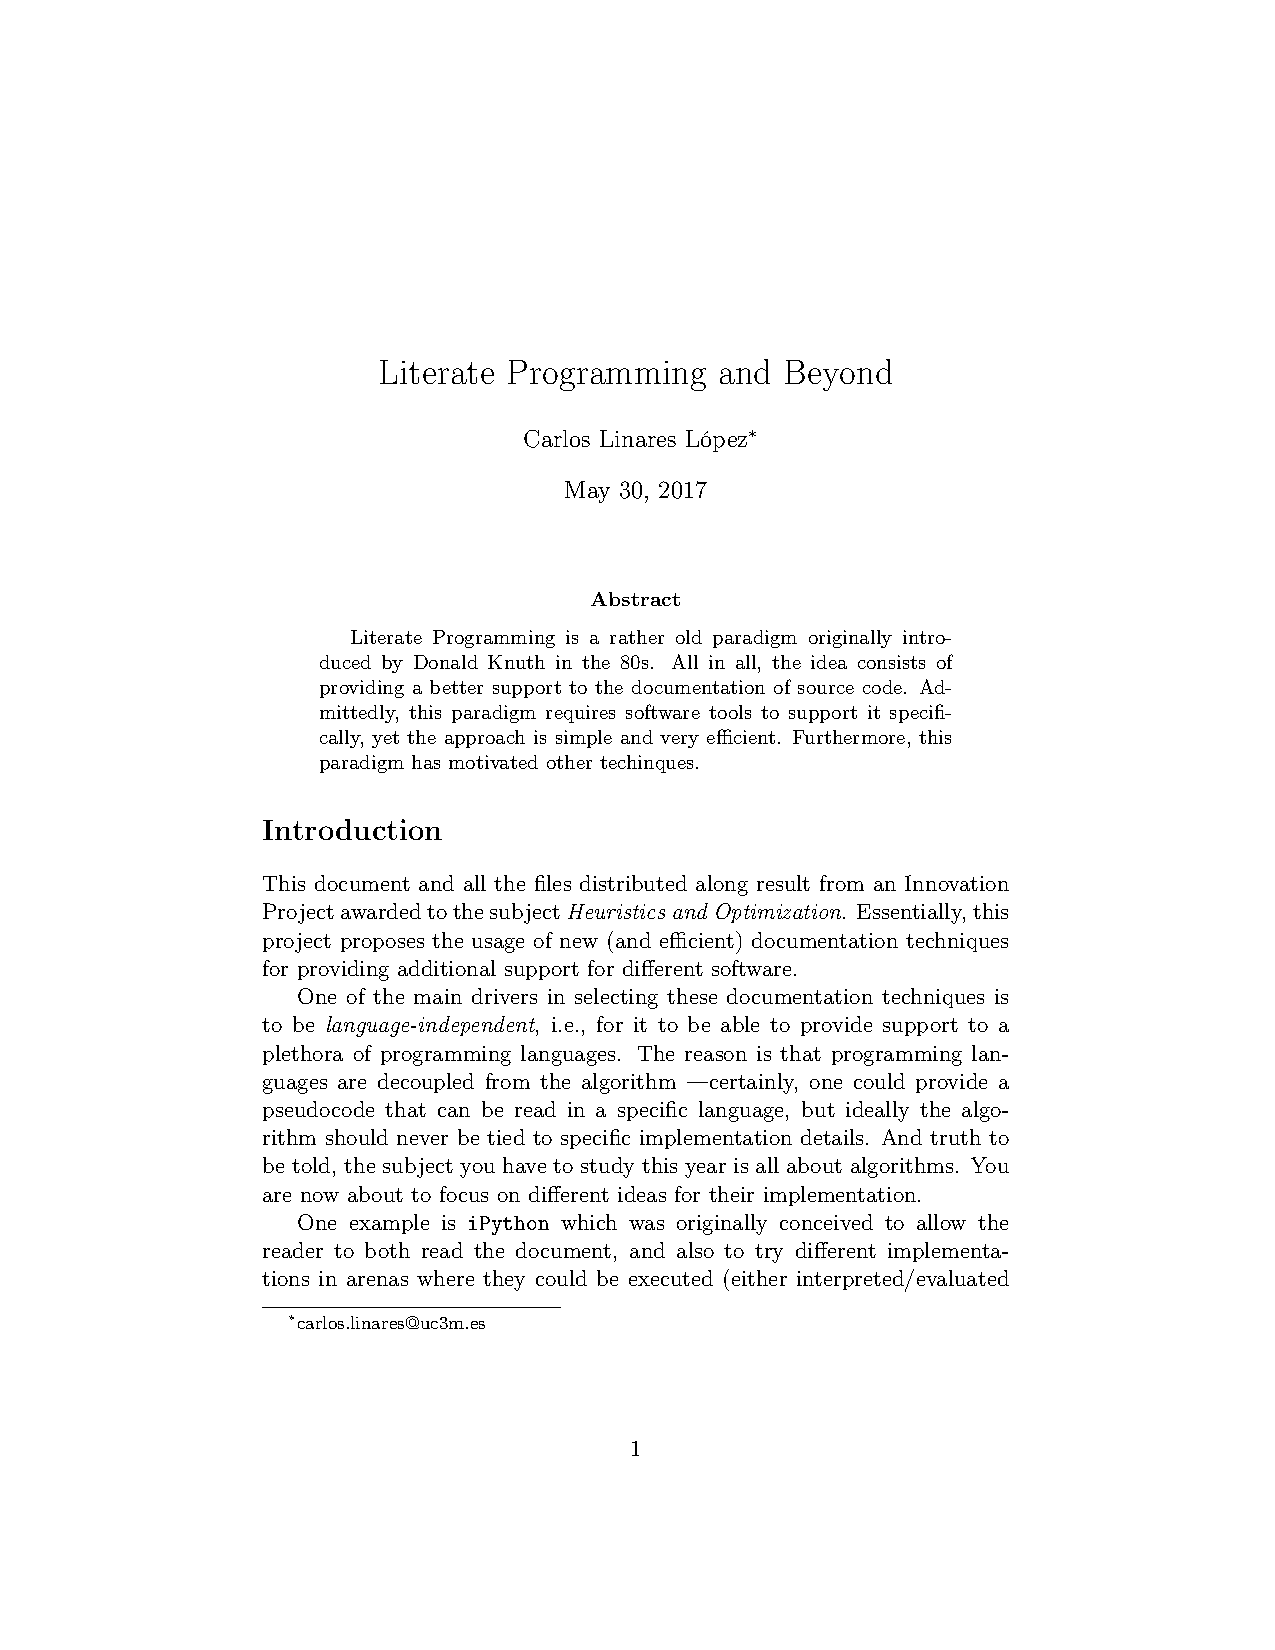
\includepdf[pages=-]{docs/intro.pdf}

\includepdf[pages=-]{docs/presentacion-es.pdf}

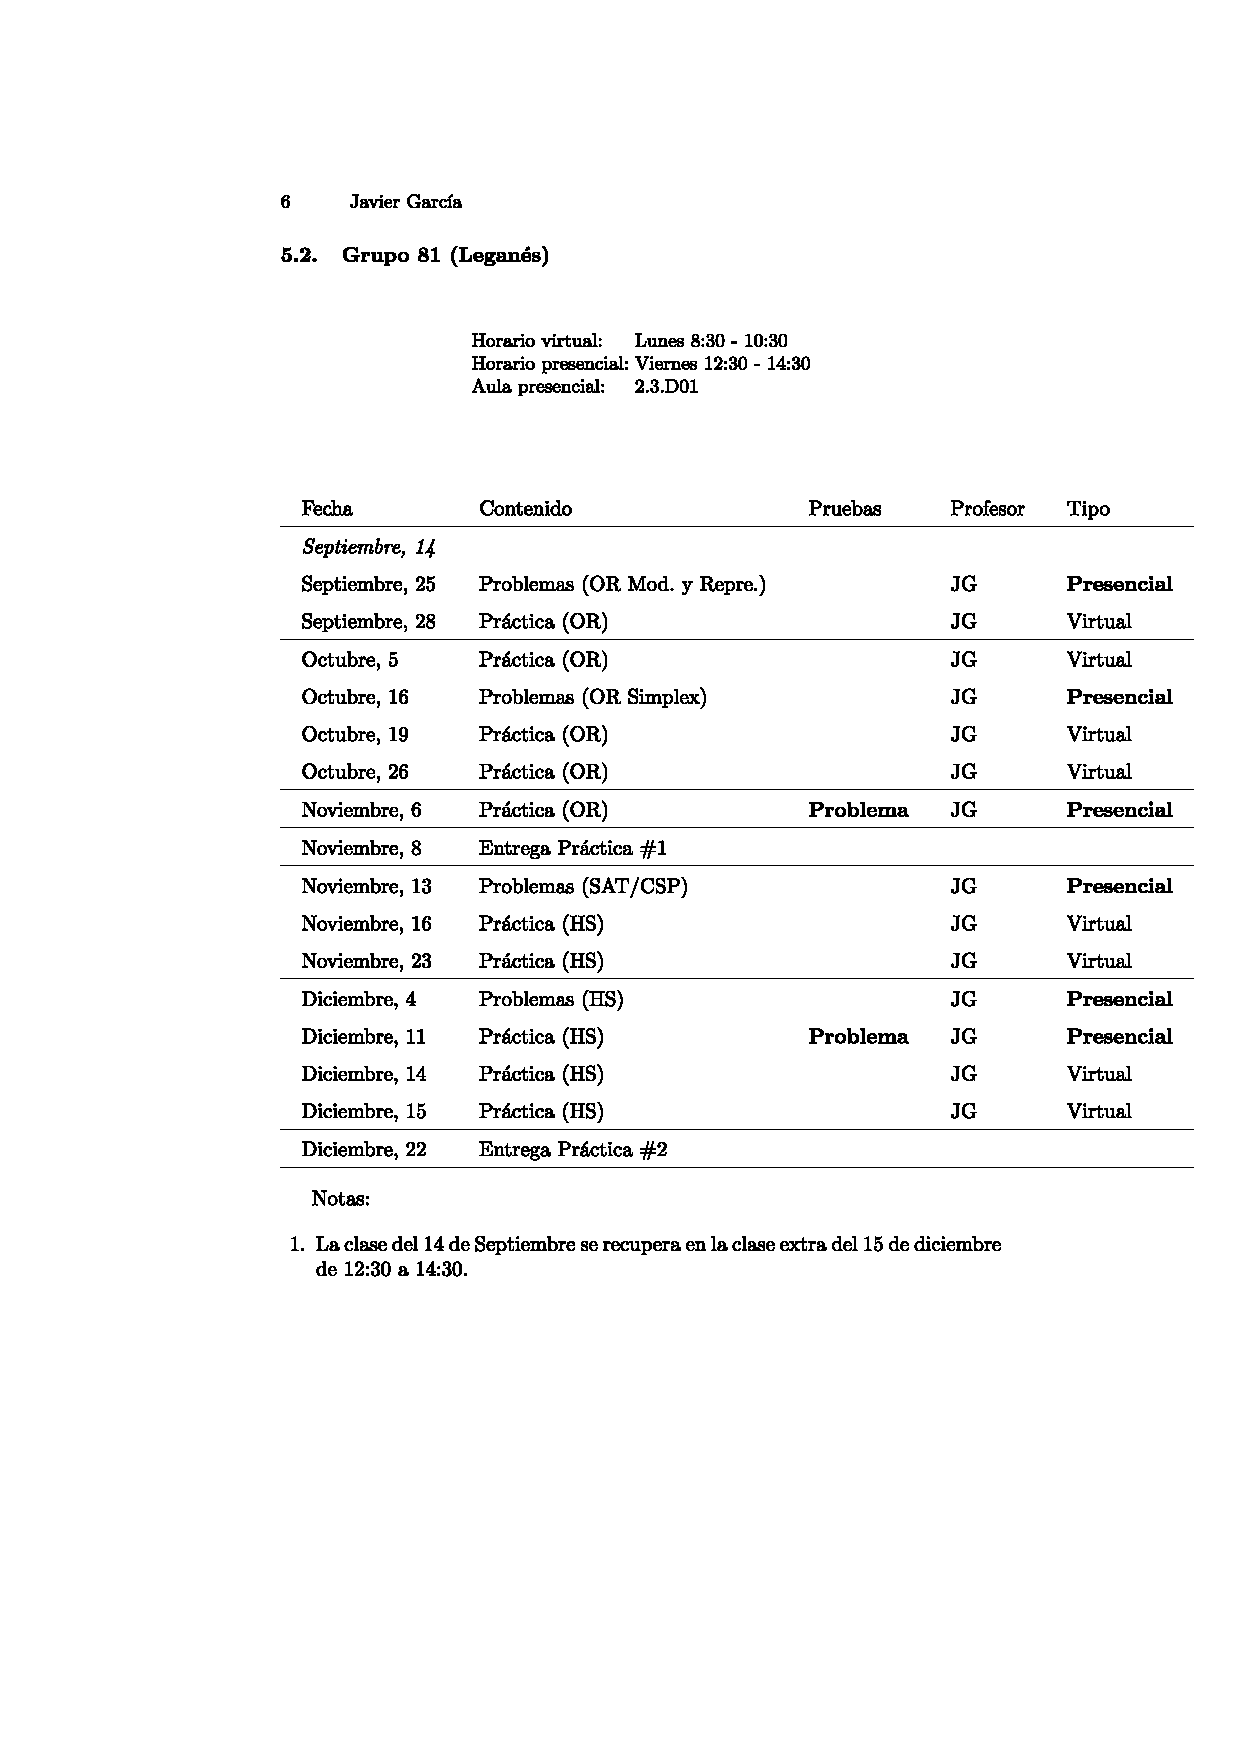
\includepdf[pages=-]{docs/HyOG81.pdf}




\part{Teoría}


\includepdf[pages=-]{docs/introduccion.pdf}


  \chapter{Tema 1 Programación Lineal}

  \section{Programación Lineal}

  \subsection{Representación grafica}


    Un problema de Programación Lineal está en Forma Canónica si y solo
    si:

    \begin{enumerate}
    \def\labelenumi{\arabic{enumi}.}
    \item
      El objetivo es de la forma de maximización.
    \item
      Si todas las restricciones son desigualdades son del tipo $\leq$.
    \item
      Si todas las variables de decisión son no negativas.
	  \begin{eqnarray*} 
		\max z = c_1x_1+c_2x_2 + \ldots +c_nx_n \\ 
		ba_{11}x_1 +a_{12}x_2 +&\ldots& +a_{1n}x_n \leq b_1 \\ 
		a_{21}x_1 +a_{22}x_2 +&\ldots& +a_{2n}x_n \leq b_2 \\ 
		&\ldots& \\ 
		a_{m1}x_1 +a_{m2}x_2 +&\ldots& +a_{mn}x_n \leq b_m \\ 
		\text { donde } x_{i} \geq 0, \forall i=1, \ldots, n
	  \end{eqnarray*}
    \end{enumerate}

    \begin{itemize}
  
    \item
      Nomenclatura:

      \begin{itemize}
    
      \item
        z representa la función a maximizar.
      \item
        Las restricciones son para un sujeto a.
      \item
        Cada fila representa una restricción.
		\item Las b's son términos escalares, racionales que deben ser menores. -
		\item Las c's son coeficientes, números racionales.
      \end{itemize}
    \end{itemize}    

    \begin{itemize}
  
    \item
      Algebraicamente:

      \begin{itemize}
      \item
        OJO: Todas deben ser del mismo tipo \textless{} o \textgreater{}
		\begin{eqnarray*} 
			\max z &=& C^{T}x \\  
			Ax\leq b&,& ejem: \begin{pmatrix}  a_{11} & a_{12} \\  
			a_{21} & a_{22}  \end{pmatrix} \cdot \begin{pmatrix}  x_1\\  
			x_2  \end{pmatrix} \leq \begin{pmatrix}  b_1\\  
			b_2  \end{pmatrix}\\  
			\text { donde } x_{i} &\geq& 0, \forall i=1, \ldots, n
		\end{eqnarray*}
      \item
        z: función objetivo.
      \item
        C: coeficientes de la función objetivo. nx1
      \item
        X: variables de decisión. nx1
      \item
        A: matriz de coeficientes tecnológicos. mxn
	  \item b: recursos. mx1
      \end{itemize}
    \end{itemize}

	\subsubsection{Desarrollo}

	
      Representar todas las restricciones en un plano como rectas,
      también x, y\textgreater0.

      \begin{itemize}
    
      \item
        Después de trazar las rectas dar valor a las variables de
        decisión y ver que hiperplano es el que cumple cada restricción
        y el área que encierren todas es la Región Factible.
      \end{itemize}

	  Por el teorema de Dantzig:

      \begin{itemize}
    
      \item
        La Región Factible es siempre un poliedro convexo.~Por lo tanto,
        uno de los vértices es la solución óptima.
      \end{itemize}

	  Solo evaluamos los puntos extremos, por lo que hay que hallar las
      intersecciones de las rectas si todavía no las conocemos.
	  \begin{itemize}
		  \item Para hallar una intersección: 
		  \begin{itemize}
			  \item Se hace un sistema con ambas
			  ecuaciones de recta. Los valores obtenidos son las intersección.
			  \begin{eqnarray*}
				\textit{Este es el metodo}\left\{\begin{matrix}
					\left\{\begin{matrix}
					-2x+y=-8\\ 
					-x+6y=18
					\end{matrix}\right.
					,
					\begin{pmatrix}
					-2 & 1 \\ 
					-1 & 6
					\end{pmatrix}
					\begin{pmatrix}
					x \\ 
					y
					\end{pmatrix}
					=
					\begin{pmatrix}
					-8 \\ 
					18
					\end{pmatrix}\\ 
					\begin{pmatrix}
					-2 & 1 \\ 
					-1 & 6
					\end{pmatrix}^{-1}
					\begin{pmatrix}
					-2 & 1 \\ 
					-1 & 6
					\end{pmatrix}
					\begin{pmatrix}
					x \\ 
					y
					\end{pmatrix}
					=
					\begin{pmatrix}
					-2 & 1 \\ 
					-1 & 6
					\end{pmatrix}^{-1}
					\begin{pmatrix}
					-8 \\ 
					18
					\end{pmatrix}\\ 
					\begin{pmatrix}
					x \\ 
					y
					\end{pmatrix}
					=
					
					\begin{pmatrix}
					-8 \\ 
					18
					\end{pmatrix}\end{matrix}\right.
			  \end{eqnarray*}
			  \item
			  \(x= A^{-1}b\); A es la matriz de coeficientes de las dos rectas
			  y b los recursos de cada una.
		  \end{itemize}
		 
	  \end{itemize}


	  Sustituimos los distintos puntos extremos (x, y, \ldots) en la
      función objetivo.

	
  Observamos todos los resultados y el máximo, será aquel de mayor
  valor.

  \begin{itemize}
  \item La solución óptima es la última vez que la curva de
  isobeneficio toca la región factible.
  \begin{figure}[H]
	\ffigbox[\FBwidth]
	{\caption{Representación PL}}
	{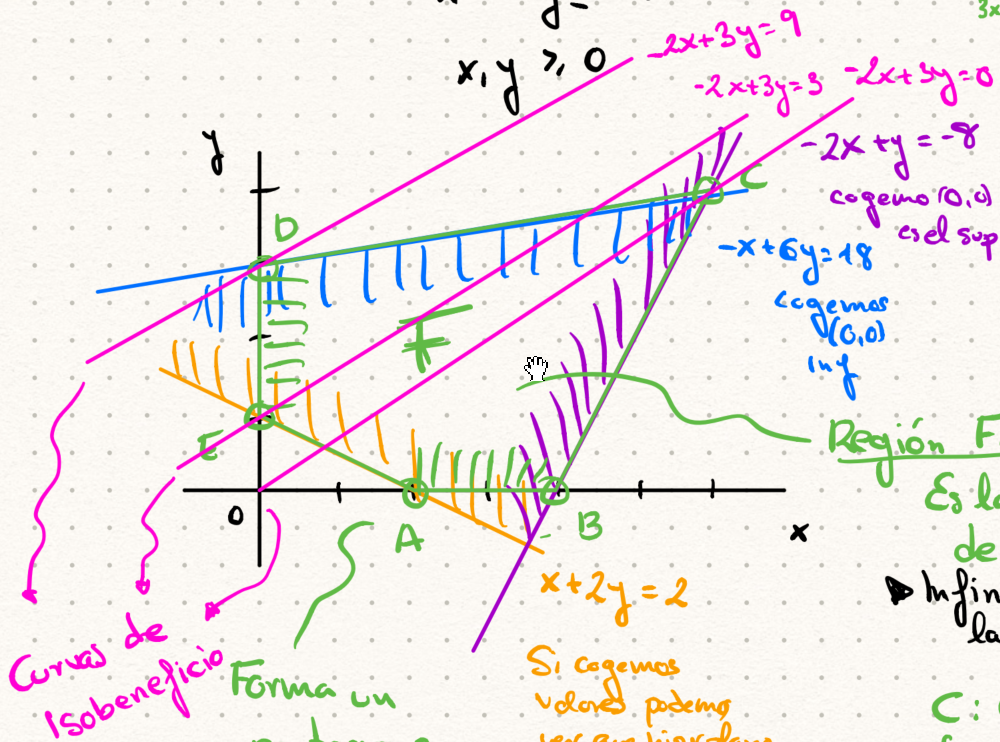
\includegraphics[scale=.2]{Untitled 1.png}}
\end{figure}
  \end{itemize}
  Ejemplo
  \begin{figure}[H]
	\ffigbox[\FBwidth]
	{\caption{Representación Programación Lineal}}
	{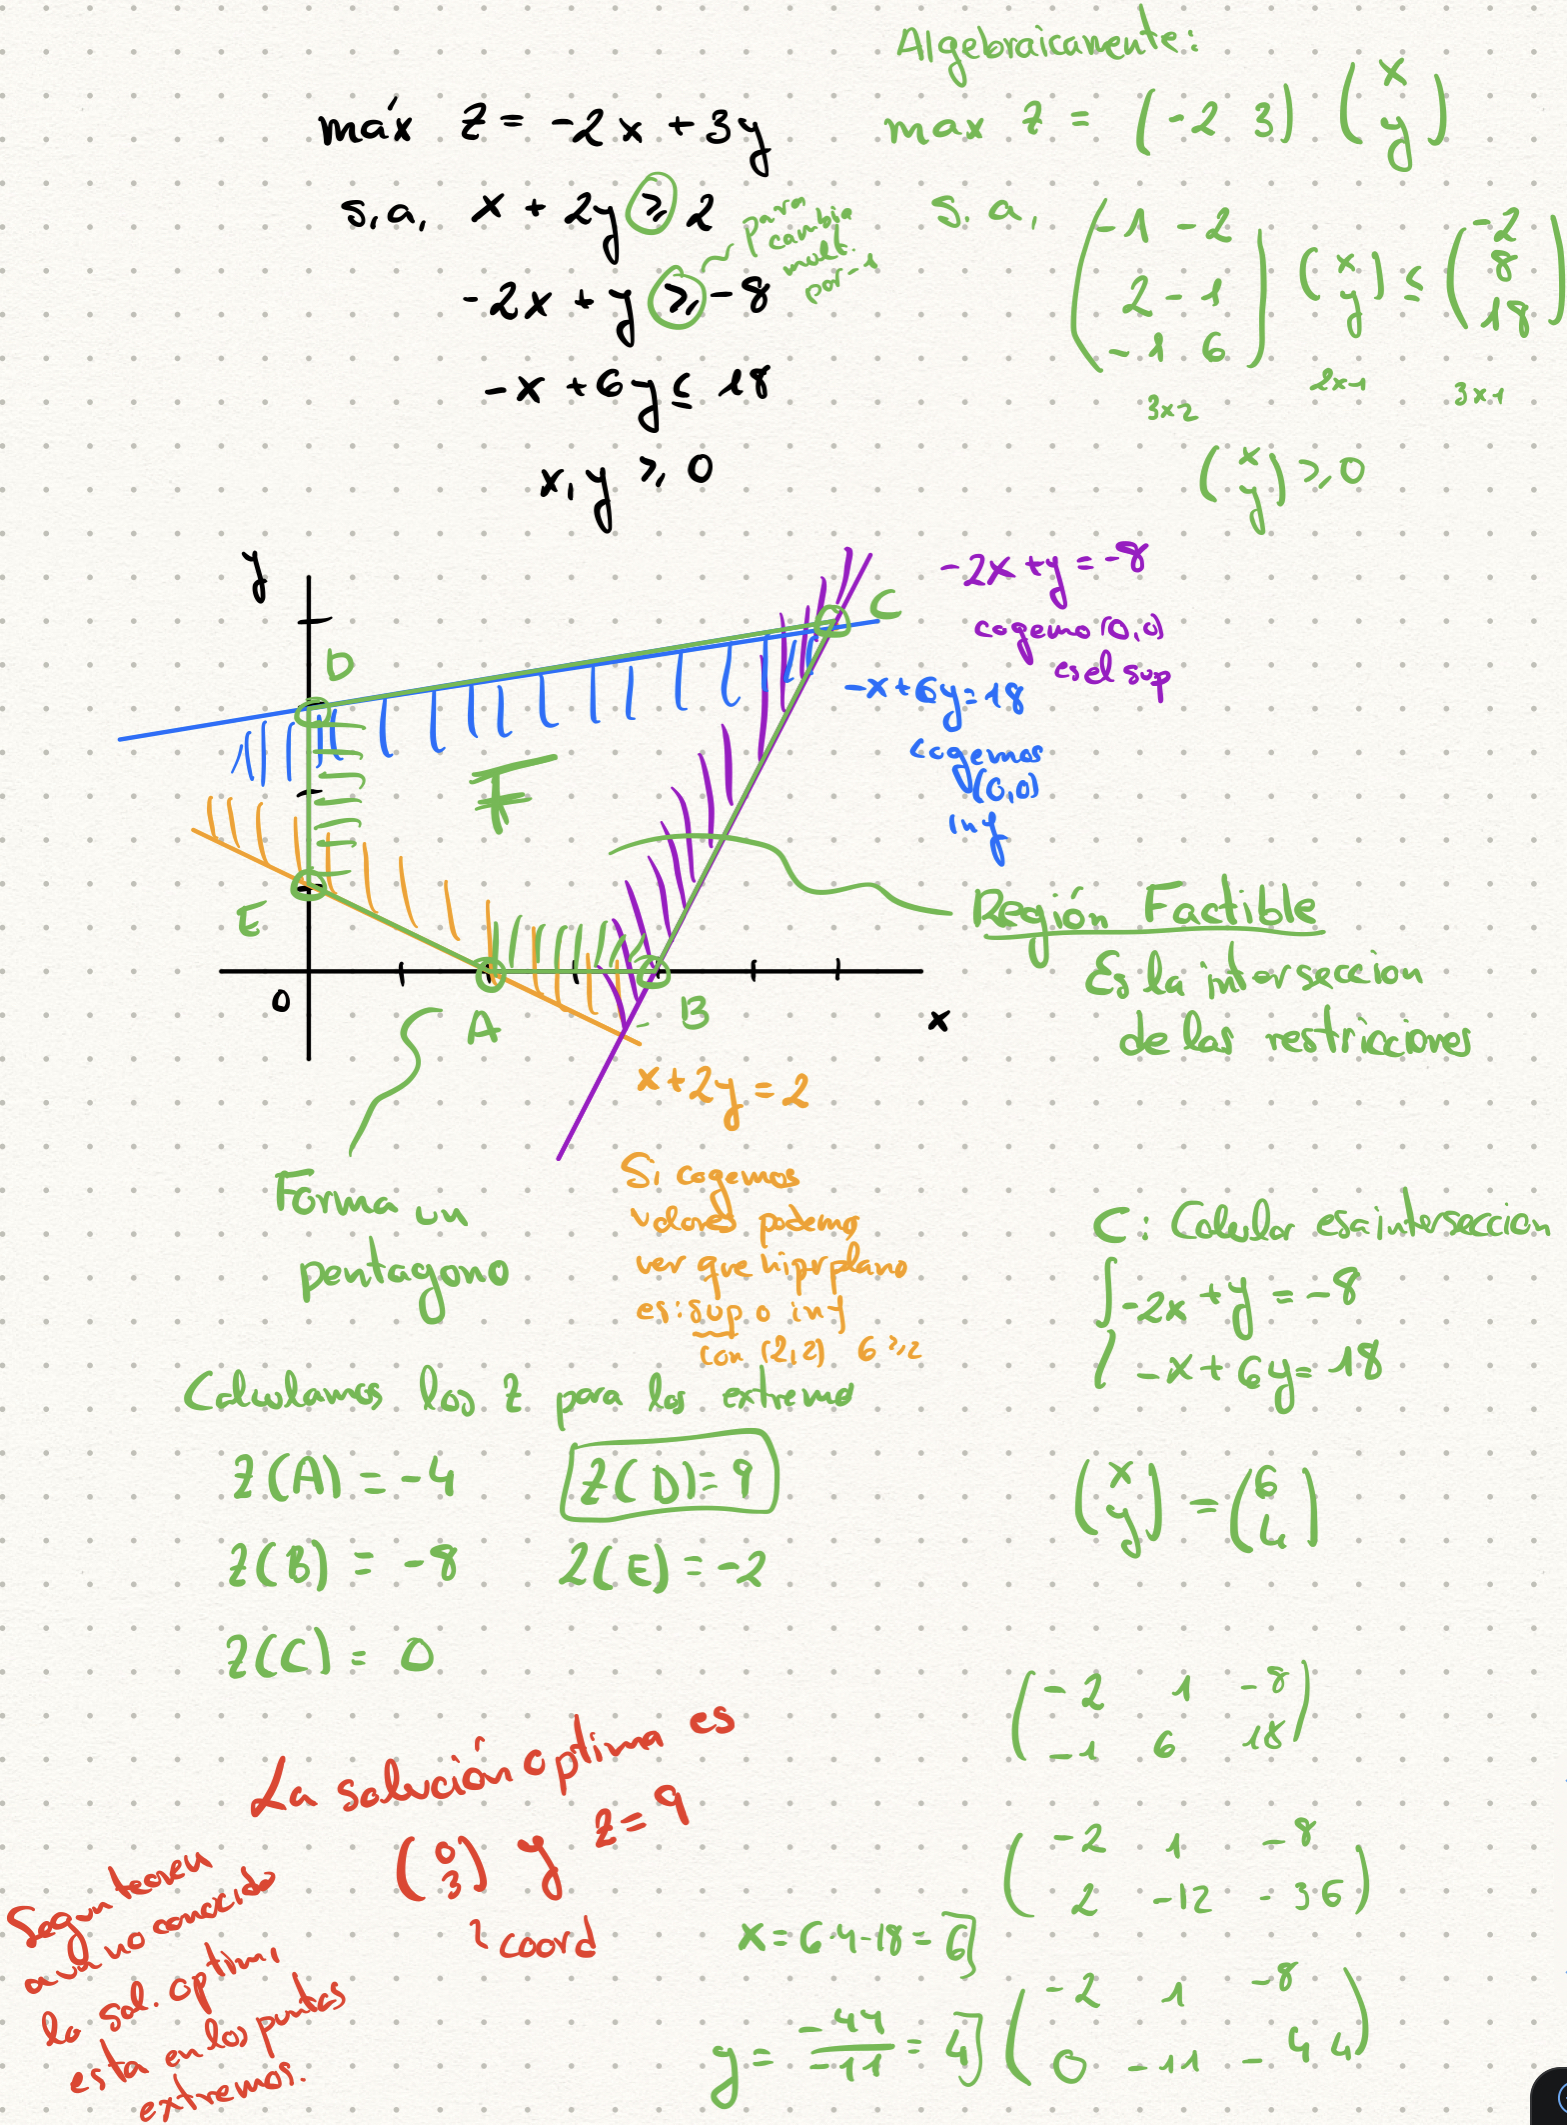
\includegraphics[scale=.3]{C96D1F11-207B-43BF-A121-0E3028966D13.jpeg}}
\end{figure}

  \subsubsection{Región factible} 
  Es la intersección de las restricciones en forma de
  semiplanos. Son los infinitos puntos que cumplen las restricciones,
  cada uno es Solución factible.


  
 \subsubsection{Soluciones}

	\paragraph{Compatible Determinado}
	Solución única.
	\begin{figure}[H]
		\ffigbox[\FBwidth]
		{\caption{Compatible Determinado}}
		{\begin{tikzpicture}[scale=.8]
			\begin{axis}[
				xlabel={$x$},
				ylabel={$y$},
				legend pos=north west,
				ymajorgrids=true,
				xmajorgrids=true,
				grid style=dashed,
				axis lines=middle,
				xmin=-2, xmax=5, ymin=-1, ymax=4,
				axis x line=center,
				axis y line=center,
			]
			\addplot[thick, smooth, color=blue] 
				{x*.4+1};
			\addplot[thick, smooth, color=blue] 
				{-x+3};
			\end{axis}
		\end{tikzpicture}}
	\end{figure}
    \paragraph{Compatible Indeterminado}
	Soluciones infinitas, están superpuestas. 
	\begin{itemize}
		\item Cuando la solución óptima no es única.
		\item Se detecta
		con el método de resolución grafica si la curva de
		isobeneficio/isocoste es paralela o idéntica a una de las
		restricciones cuyos puntos extremos son soluciones optimas.

		\begin{figure}[H]
			\ffigbox[\FBwidth]
			{\caption{Compatible Determinado}}
			{\begin{tikzpicture}[scale=.8]
				\begin{axis}[
					xlabel={$x$},
					ylabel={$y$},
					legend pos=north west,
					ymajorgrids=true,
					xmajorgrids=true,
					grid style=dashed,
					axis lines=middle,
					xmin=-2, xmax=5, ymin=-1, ymax=4,
					axis x line=center,
					axis y line=center,
				]
				\addplot[thick, smooth, color=blue] 
					{x*.4+1};
				\end{axis}
			\end{tikzpicture}}
		\end{figure}
	\end{itemize}
	
    No acotado, faltan restricciones y hay soluciones infinitas
	\begin{figure}[H]
		\ffigbox[\FBwidth]
		{\caption{Compatible Determinado}}
		{\begin{tikzpicture}[scale=.8]
			\begin{axis}[
				xlabel={$x$},
				ylabel={$y$},
				legend pos=north west,
				ymajorgrids=true,
				xmajorgrids=true,
				grid style=dashed,
				axis lines=middle,
				xmin=-2, xmax=5, ymin=-1, ymax=4,
				axis x line=center,
				axis y line=center,
			]
			\addplot[thick, smooth, color=blue] 
				{x*1.4+1};
			\addplot[thick, smooth, color=blue] 
				{x*1.8-3};
			\addplot[thick, smooth, color=blue] 
				{-x+1};
			\end{axis}
		\end{tikzpicture}}
	\end{figure}
    

	Incompatible: 
	\begin{itemize}
		\item Infactible 
		\begin{itemize}
			\item Si y solo si la región de soluciones
			factibles es vacía: \(F=\emptyset\), ya sea porque no cortan o
			porque cortan en zonas negativas.
			\begin{figure}[H]
				\ffigbox[\FBwidth]
				{\caption{Compatible Determinado}}
				{\begin{tikzpicture}[scale=.8]
					\begin{axis}[
						xlabel={$x$},
						ylabel={$y$},
						legend pos=north west,
						ymajorgrids=true,
						xmajorgrids=true,
						grid style=dashed,
						axis lines=middle,
						xmin=-2, xmax=5, ymin=-1, ymax=4,
						axis x line=center,
						axis y line=center,
					]
					\addplot[thick, smooth, color=blue] 
						{x*1.4+1};
					\addplot[thick, smooth, color=blue] 
						{x*1.4-3};
					
					\end{axis}
				\end{tikzpicture}}
			\end{figure}
		\end{itemize}

	\end{itemize}

	
	
  El método de resolución grafica solo es posible para como mucho 3
  variables de decisión.
\pagebreak
  \subsection{Transformaciones}

  
  Pasar inecuaciones de un tipo a otro (para Forma Canónica)

  $$\begin{aligned}  &\sum_{j=1}^{n} a_{i j} x_{j} \geqslant b_{i} \triangleq -\sum_{j=1}^{n} a_{i j} x_{j}\leq -b_{i}  \end{aligned}$$

	Transformar maximización en minimización y viceversa:

	
	$$\min z = C^{T}x \triangleq \max z =- C^{T}x$$

  Quitar inecuación (para Forma Estándar)

  $$\begin{aligned}  &\sum_{j=1}^{n} a_{i j} x_{j} \leqslant b_{i} \triangleq \sum_{j=1}^{n} a_{i j} x_{j}+s_{i}=b_{i}\\  &\sum_{j=1}^{n} a_{i j} x_{j} \geqslant b_{i} \triangleq \sum_{j=1}^{n} a_{i j} x_{j}-s_{i}=b_{i}  \end{aligned}s_i: \textit{variables de holgura. Son variables de decisión cuando}$$
  
  operamos.

  
Poner inecuación a partir de igualdad:

  \(\sum_{j=1}^{n} a_{i j} x_{j} = b_{i}\) es
  \(\sum_{j=1}^{n} a_{i j} x_{j} \leqslant b_{i}\) y
  \(\sum_{j=1}^{n} a_{i j} x_{j} \geq b_{i}= -\sum_{j=1}^{n} a_{i j} x_{j} \leqslant b_{i}\)

  Si una variable de decisión \(x_i\) no está restringida se pone
  entonces como la diferencia de dos variables no negativas
  restringidas: \(x_i=x_i'-x_i''; x_i',x_i'' \geq 0\)

  
\subsection{Método Simplex}

Simplex: Poliedro convexo de n dimensiones.

    Una tarea de Programación Lineal está en Forma Estándar ( de
    maximización / minimización) si y solo si:

	
  \begin{enumerate}
  \def\labelenumi{\arabic{enumi}.}

  \item
    La función objetivo es de maximización (minimización, si se dice
    forma estándar se supone siempre maximización a menos que lo digan
    explícitamente).

    
  
    \item
      Todas las restricciones son =.
    \item
      Todas las variables de decisión son no negativas.
    \item
      Todos los recursos son no negativos.
  \end{enumerate}

    Algebraicamente:

    $$\begin{aligned}  &\max z = C^{T}x \\  &Ax = b \\ &x, y\geqslant 0 \end{aligned}$$
	\begin{figure}[H]
		\ffigbox[\FBwidth]
		{\caption{Representación Simplex}}
		{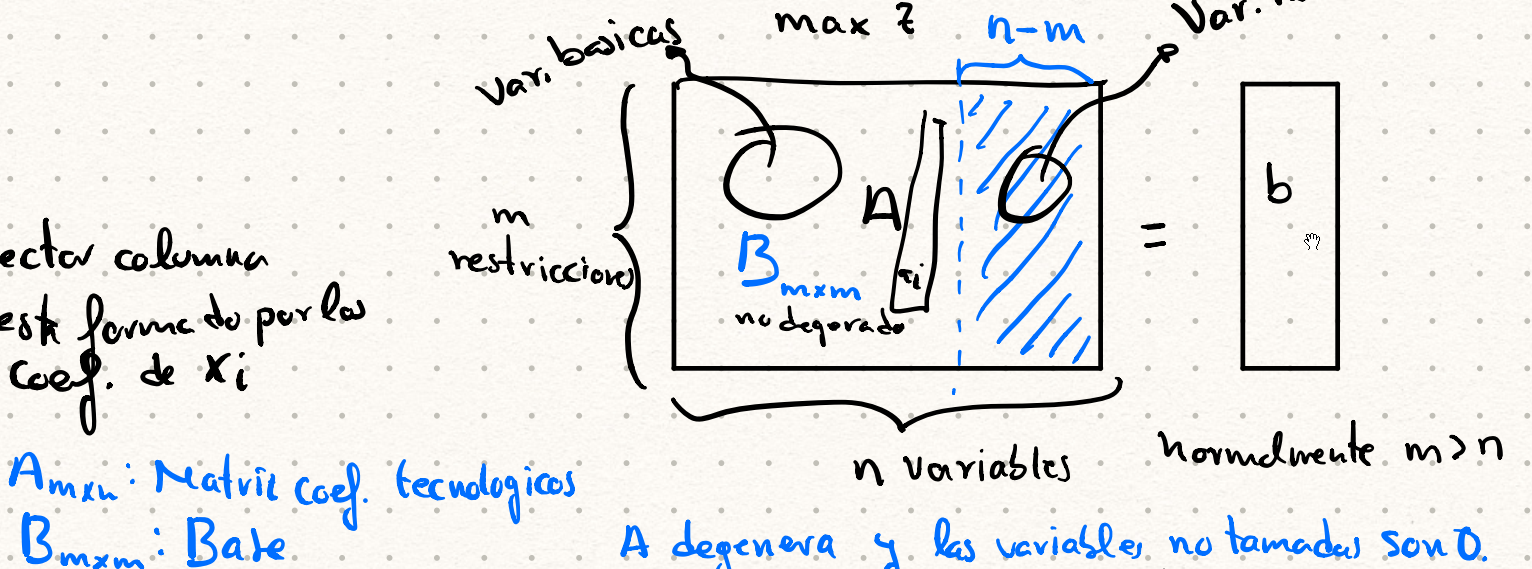
\includegraphics[scale=.3]{Untitled 9.png}}
	\end{figure}

	Teorema George Dantzig: Dado una tarea de Programación lineal en forma
  estándar, el valor óptimo si lo hubiera, se alcanza en un punto
  extremo de la región factible.


  
    Términos:
	\begin{itemize}
		\item Variable básica: Que no toma valor 0.
		\item
		Variable no básicas: Son las que toman valor 0.
	  \item
		\(a_i\): Vector columna, está formado por los coeficientes de
		\(x_i\) de las restricciones.
	  \item
		\(c_i\): Coeficientes de la \(x_i\) de la función objetivo.
	  \item
		\(i\): variables básicas.
	  \item
		\(j\): variables no básicas.
	\end{itemize}

	\pagebreak
    Tipos de soluciones:

    \begin{itemize}
    \item
      Definición 4
	  \begin{figure}[H]
		\ffigbox[\FBwidth]
		{\caption{Definición 4}}
		{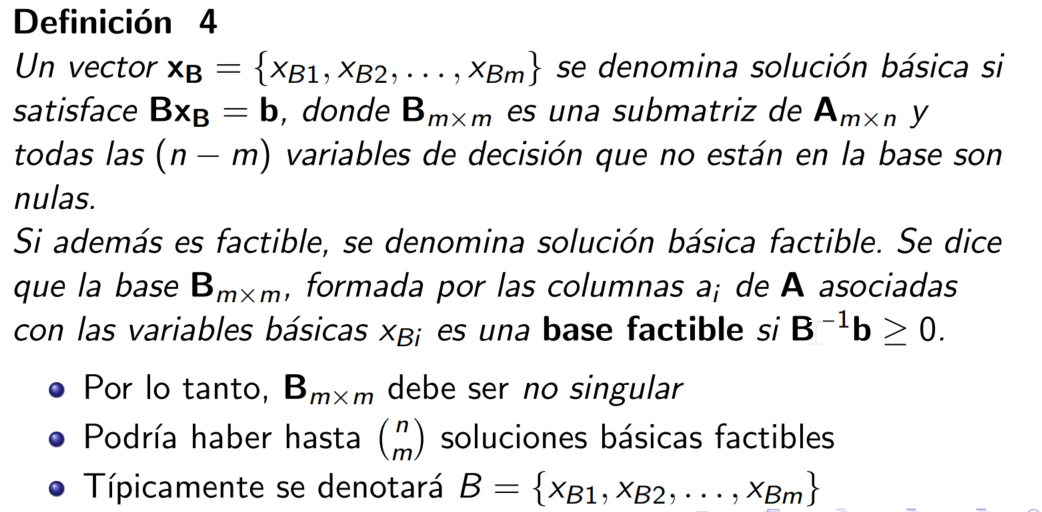
\includegraphics[scale=.3]{Untitled 10.png}}
	\end{figure}
	  \begin{itemize}
		  \item Un vector \(x\) que satisface \(Ax=b\) se llama Solución.
		  \item Un vector \(x_B\) que satisface \(Bx_B=b\) se llama Solución Básica.
		  \item Un vector \(x_B \geq 0\) que satisface \(Bx_B=b\) se llama Solución Básica Factible.
	  \end{itemize}
    \end{itemize}

	
    Cálculo de la función objetivo: \(z=C_B^Tx_B\), solo se consideran
    las variables básicas.

	Una solución factible optima, \(x^*\), si y solo si:
    \(c^Tx^* \geq c^Tx; \forall \in xF\)

	Modelo iterativo:

    \begin{enumerate}
    \def\labelenumi{\arabic{enumi}.}
  
    \item
      Calcular una solución básica factible inicial.
    \item
      Si existe un punto extremo adyacente que mejore z, transitamos a
      él.
    \item
      En otro caso, detenerse.
    \end{enumerate}
\pagebreak
	Proceso normal:

    \begin{itemize}
  
    \item
      Cálculo de las variables básicas:

      \begin{enumerate}
      \def\labelenumi{\arabic{enumi}.}
    
      \item
        Seleccionar una base mxm (m: número de restricciones), matriz
        cuadrada B, que tenga inversa y no haga los recursos negativos.

        \begin{itemize}
      
        \item
          Tratamos de usar la matriz identidad.
        \item
          Variables Artificiales: Para empezar con base matriz
          identidad.

			\(t_i\) se denomina Variable artificial que se añade a la
            función objetivo con coeficiente -M, para que no salga en la
            solución.

			Añadimos a una de las restricciones que tenga una variable
            de holgura que no nos interesa para hacer la matriz básica.

			\item
          \(B = \{ x_i \}\), se recomienda escribir en orden de índice.
        \end{itemize}
      \item
        Calculamos el valor de las variables básicas de la solución
        básica factible, \(x_B=B^{-1}b\).
      \item
        Hallamos el valor de la función objetivo para esta solución
        básica factible, \(z_B=C_B^Tx_B\)
      \end{enumerate}
    \item
      Selección de la variable de entrada: Buscamos un punto extremo
      adyacente que mejore la z, evaluamos las variables no básicas.

      \begin{enumerate}
      \def\labelenumi{\arabic{enumi}.}
    
      \item
        Calculamos los costes reducidos para las variables no básicas,
        \(z_j-c_j\)

        $$\begin{matrix}
			z_j=C_B^Ty_j\\ 
			y_j=B^{-1}a_j
		\end{matrix}$$
      \item
        La variable de entrada será:

        \begin{itemize}
      
        \item
          En max. se coge el más negativo y el proceso terminara cuando
          todos son positivos.
        \item
          En min. se coge el más positivo y el proceso termina cuando
          todos los costes sean negativos.
        \end{itemize}
      \end{enumerate}
    \item
      Regla de salida: Para que tenga dimensión m tenemos que sacar una
      variable básica de la base.

      \begin{itemize}
    
      \item
        La variable que salga de la base, será:
        \(min\{ \frac {x_i} {y_{i'}} \}\) , con \(y_{i'} \geq 0\).
      \end{itemize}
    \end{itemize}
\pagebreak
	Proceso tabular:
	\begin{figure}[H]
		\ffigbox[\FBwidth]
		{\caption{Simplex Tabular}}
		{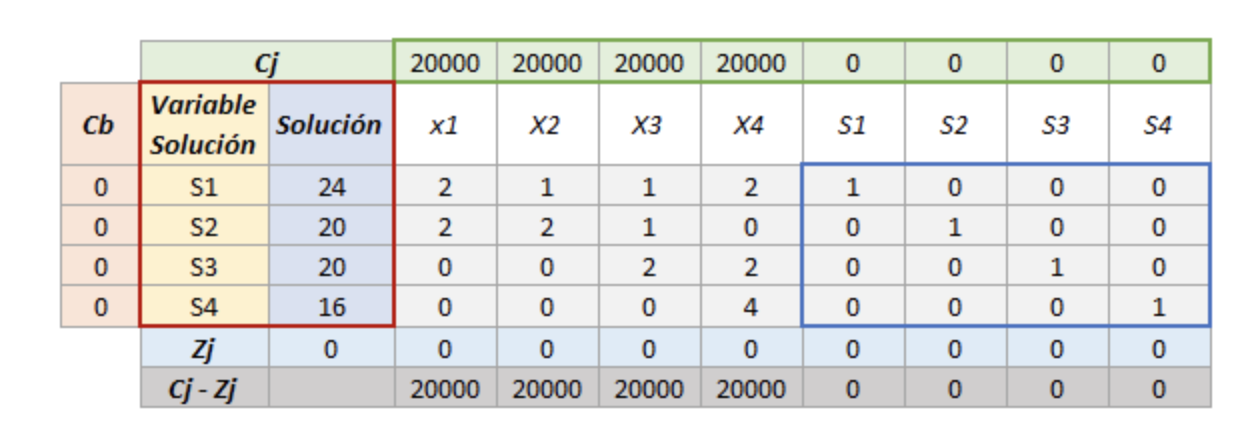
\includegraphics[scale=.3]{Untitled 11.png}}
	\end{figure}

  Casos de las distintas soluciones: 
 \begin{enumerate}
	 \item Dada la solución factible
	 \(x_B=B^{-1}b\) y \((z_j-c_j) > 0\). 
	 \begin{itemize}
		 \item Solución Óptima Única. 
	 \end{itemize}
	 \item Dada la solución factible \(x_B=B^{-1}b\) y \((z_j-c_j) > 0\) para todas
	 las variables no básicas salvo una o más para las que
	 \((z_j-c_j) = 0\).
	 \begin{itemize}
		\item Soluciones Optimas Infinitas. 
	\end{itemize}
	 \item Dada la solución factible \(x_B=B^{-1}b\) y \((z_j-c_j) < 0\) pero algún \(x_j\) no
	 básica con \(y_j \leq 0\).
	 \begin{itemize}
		 \item Básicamente que al intentar sacar una
		 variable todas las componentes no sean validas, ya sea porque son
		 divisiones entre 0 o entre negativos y dan negat79ivos, ambas no
		 válidas. 
		 \item No Acotado. 
	 \end{itemize}
	 
	 \item Dada la solución factible \(x_B=B^{-1}b\) y
	 \((z_j-c_j) \geq 0\), pero alguna variable artificial toma valor
	 positivos, que tenga valor en la solución. Variable artificial no es
	 lo mismo que variable de holgura, las artificiales son para comenzar
	 por la identidad y aportan negativamente a la función objetivo.
	 \begin{itemize}
		\item Infactible, región factible vacía.
	\end{itemize} 	 
 \end{enumerate} 
\pagebreak
\subsection{Dualidad}

Una tarea de Programación Lineal está en Forma Simétrica o Forma
Canónica de maximización (o minimización si se dice explícitamente) si
y solo si: 

\begin{enumerate}
	\item El objetivo es de la forma de maximización.
	\item Si todas las restricciones son desigualdades son del tipo $\leq$.
	\item Si todas las variables de decisión son no negativas.
\end{enumerate}

El Problema Dual del Problema Primal (el canónico o simétrico):

\begin{minipage}{.5\linewidth}
	$$\max z = C^{T}x \\  
	Ax\leq b \\ 
	x_{i} \geq 0$$
\end{minipage}
es
\begin{minipage}{.5\linewidth}
	$$\min w = b^{T}x' \\ 
	A^Tx' \geq c \\ 
	x' \geq 0$$
\end{minipage}

Si la tarea de Programación Lineal en Forma Simétrica tiene una
solución óptima correspondiente a una base B, entonces:
\(x'^*= c_B^TB^{-1}\)
\begin{figure}[H]
	\ffigbox[\FBwidth]
	{\caption{Dualidad}}
	{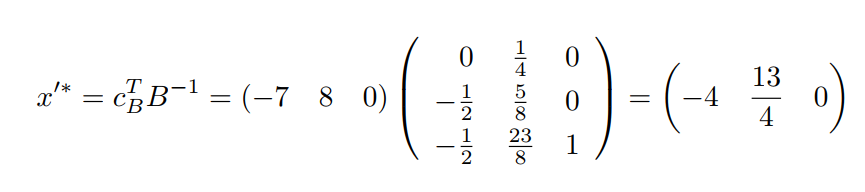
\includegraphics[scale=.4]{Untitled 14.png}}
\end{figure}

\begin{itemize}

	\item c y B, son las del problema resuelto, los que ya conocíamos. No las
	del problema simétrico.
	\item Teorema: la variable dual \(x_i'^*\) indica la contribución al
	crecimiento de la función objetivo por unidad del recurso i-esimo
	(de la primal, no la dual).
	\begin{itemize}
		\item  Nos permite saber cuándo aumenta la función objetico si le sumamos
	1 al recurso.
	\end{itemize}

\end{itemize}

\subsection{Interpretación de resultados}

Interpretación de la solución.

\begin{enumerate}
	\item Factible o Infactible. Se justifica con que no haya salido un valor positivo en las variables artificiales en la solución optima.
	\item Solución única o infinitas. Se justifica con que nos han salido
	costes reducidos estrictamente positivos en la última iteración.
 	\item Función objetivo acotable o no acotable. Se justifica con que el
	\(y_i\) de \(x_i\) no son negativos o nulos, por lo que se ha
	podido elegir una variable de salida.
\end{enumerate}

Interpretación de los recursos.

\begin{enumerate}
	\item Interpretación de las variables de holgura.
	\begin{itemize}
		\item Si la variable de holgura suma, es que sobran recursos.
		\item Si resta la variable de holgura es que falta recurso.
	\end{itemize}
	\item Dualidad: Contribución unitaria de cada recurso al crecimiento de
	la función objetivo.

	\begin{itemize}
	\item Indicar de forma individual cuales de las variables contribuyen,
		cuanto, y cuáles no.
	\end{itemize}
\end{enumerate}
\pagebreak
\subsection{Modelización}

\subsubsection{Problema de Transporte}
\begin{figure}[H]
	\ffigbox[\FBwidth]
	{\caption{Problema de Transporte}}
	{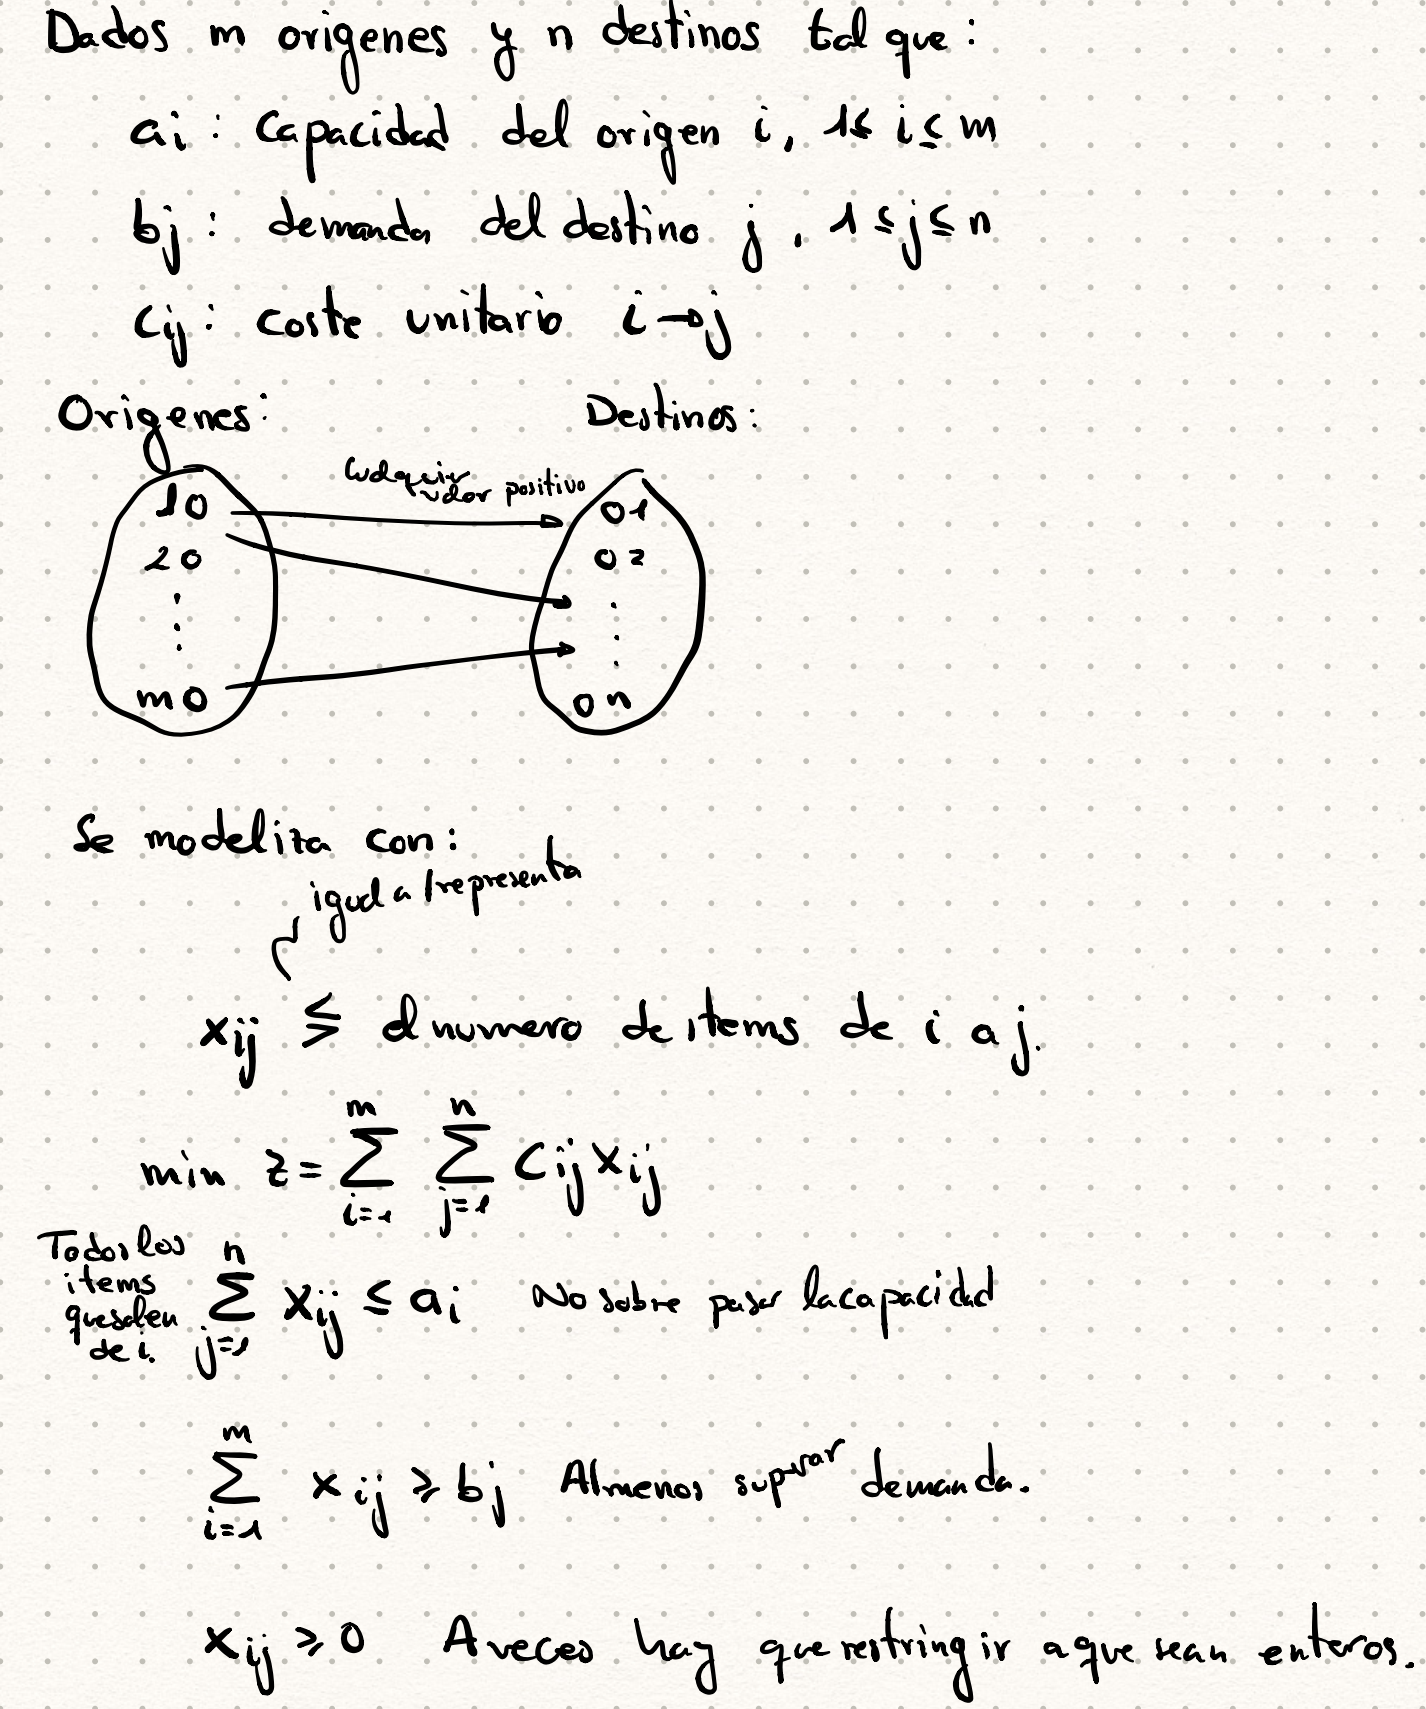
\includegraphics[scale=.25]{Untitled 15.png}}
\end{figure}
\subsubsection{Problema de Asignación}
\begin{figure}[H]
	\ffigbox[\FBwidth]
	{\caption{Problema de Asignación}}
	{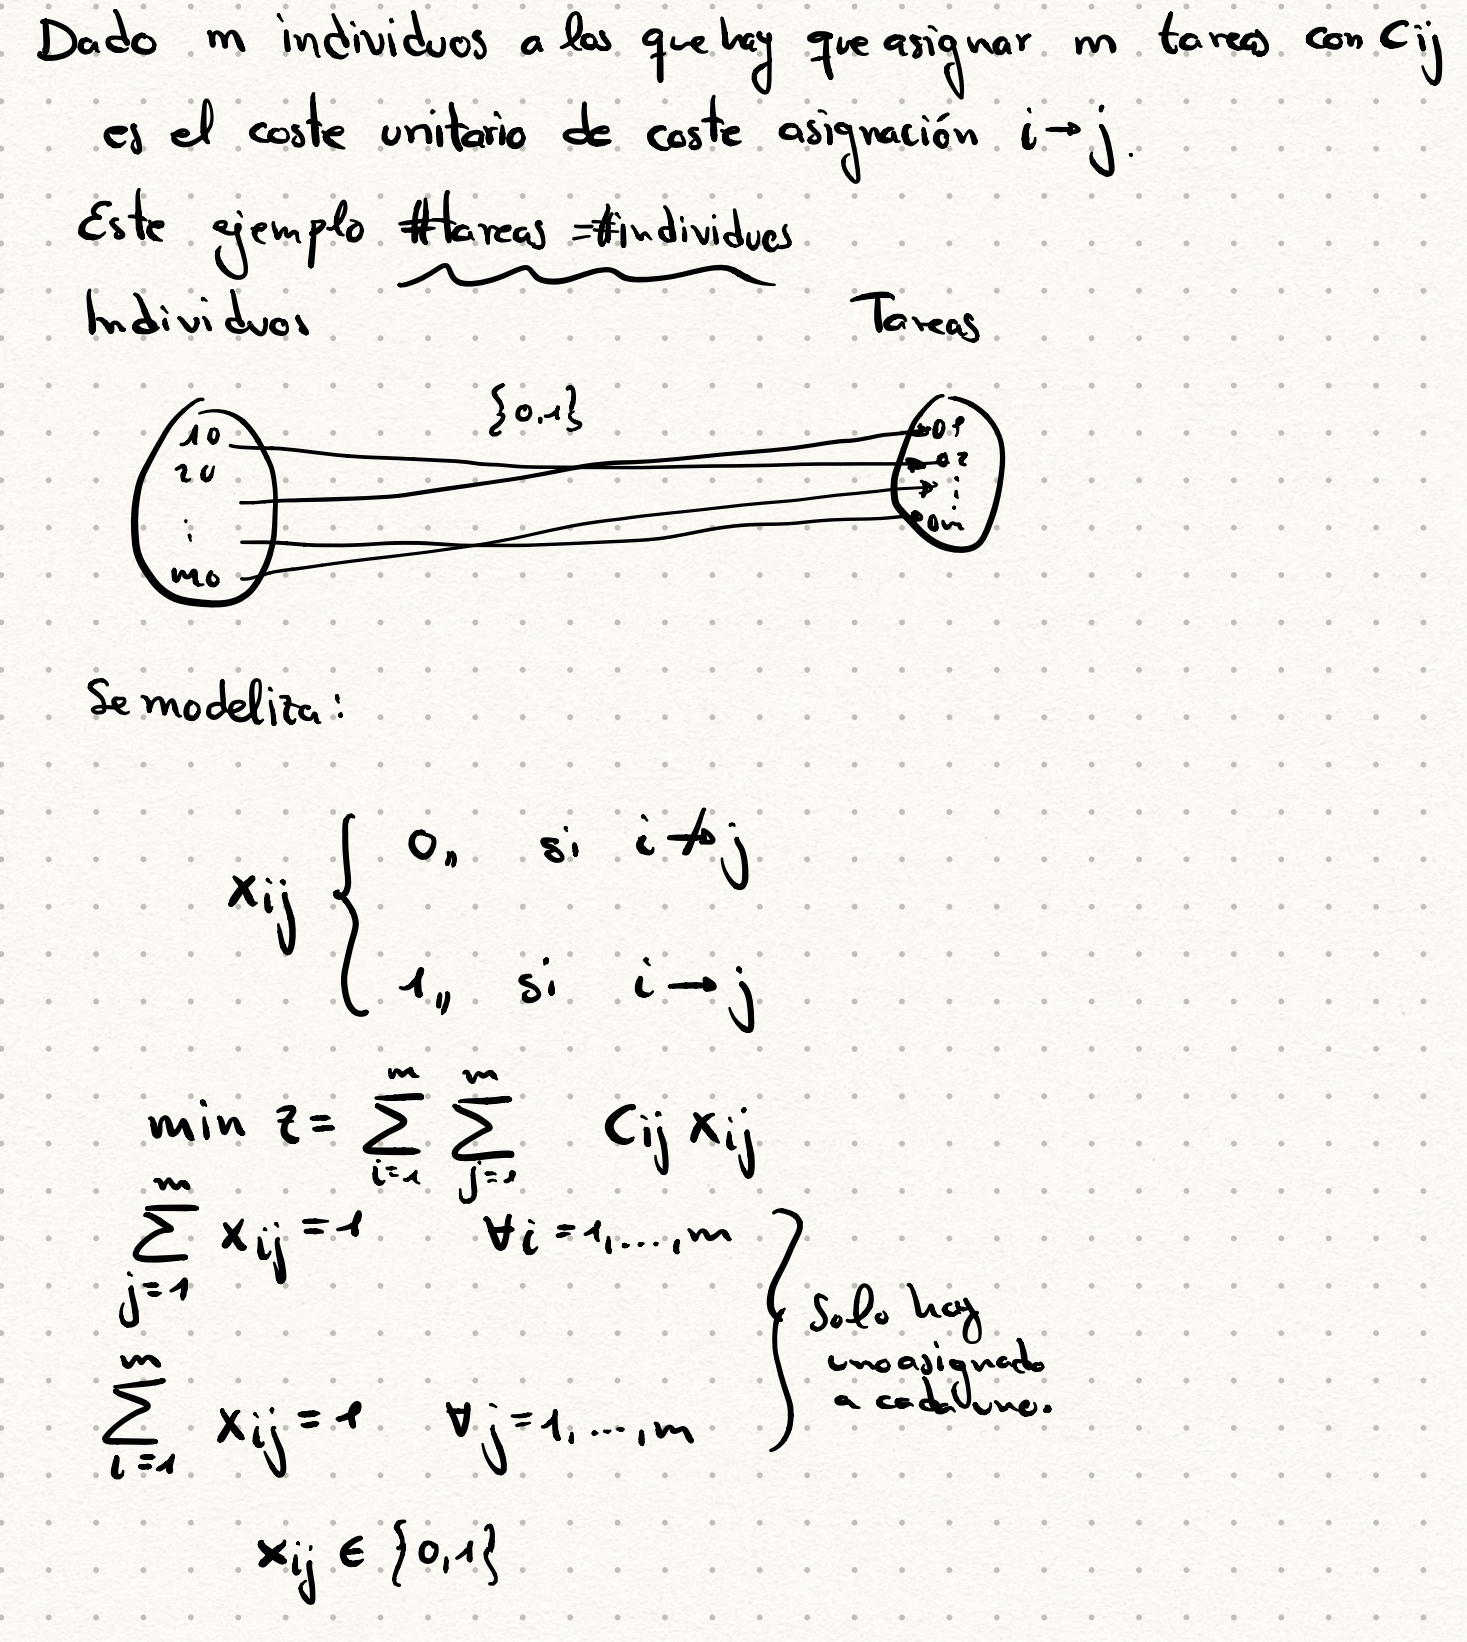
\includegraphics[scale=.25]{Untitled 16.png}}
\end{figure}
\subsubsection{Condicionales}
\begin{figure}[H]
	\ffigbox[\FBwidth]
	{\caption{Condicionales}}
	{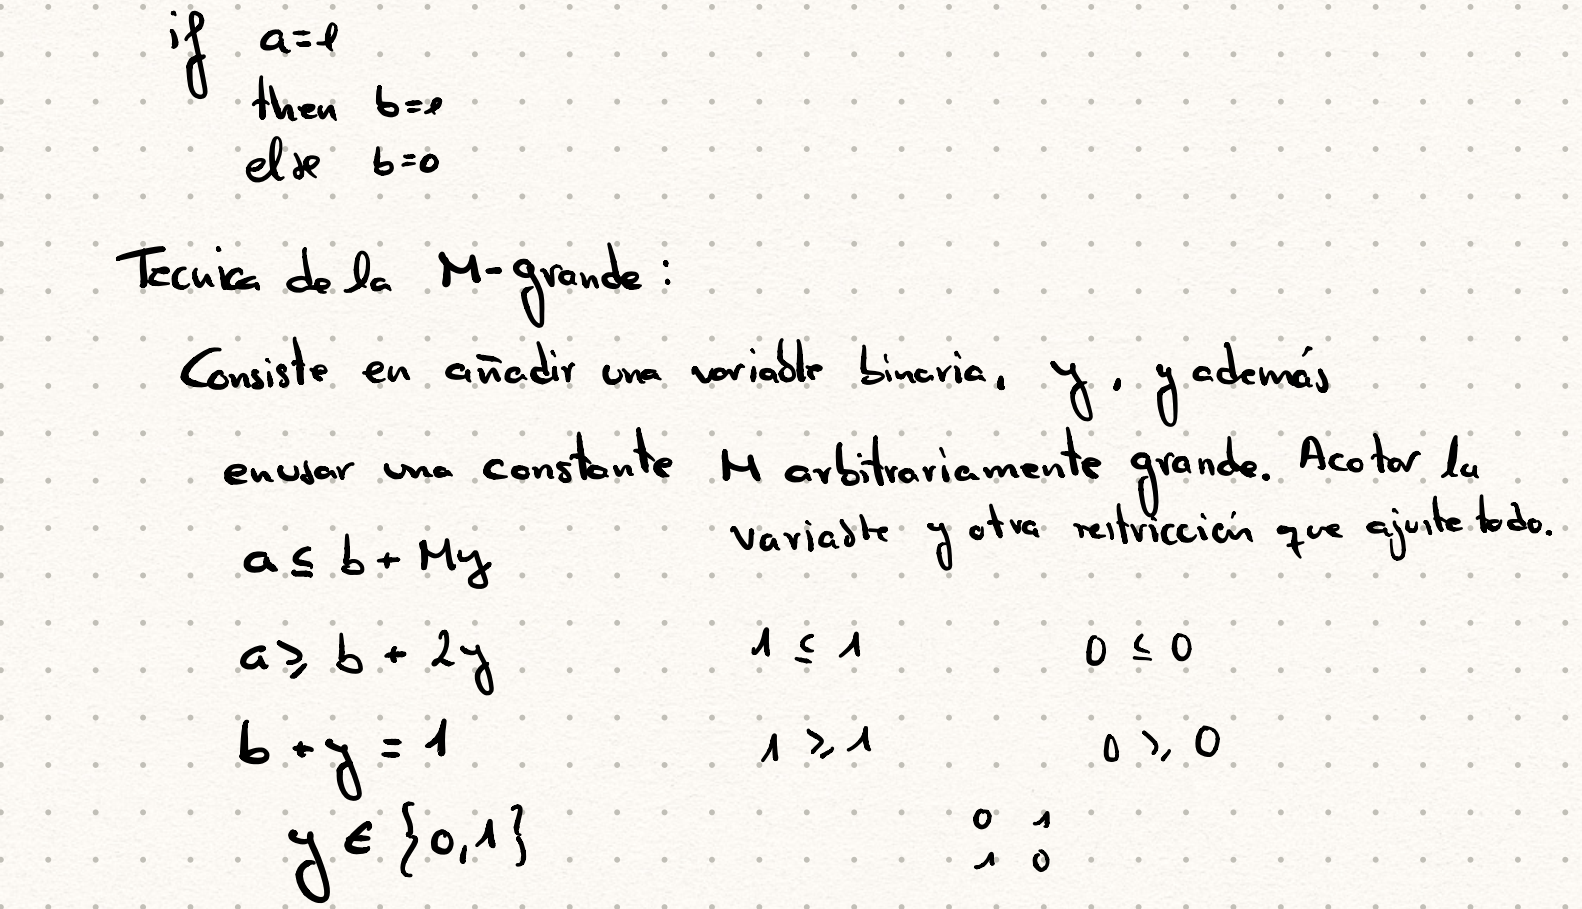
\includegraphics[scale=.25]{Untitled 17.png}}
\end{figure}
\begin{figure}[H]
	\ffigbox[\FBwidth]
	{\caption{Condicionales}}
	{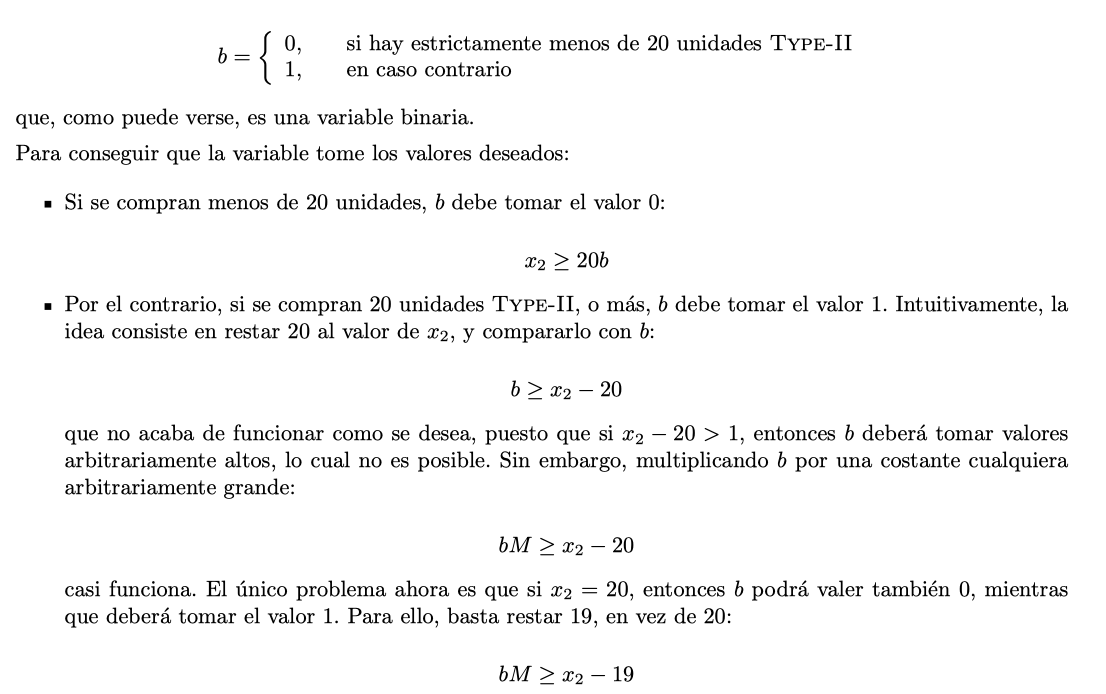
\includegraphics[scale=.6]{Screenshot_2020-11-02_at_14.40.37.png}}
\end{figure}
Lo primero es acotar la variable, $\leq$ y $\geq$.

Después con una variable binaria y la arbitrariamente grande debemos
obligar a la variable a tomar el valor que nosotros queramos.

Partiendo de la condición, miramos en que parte de la misma podemos
meter la variable binaria y que obligue a que tome 1 o 0, idealmente
ambos. Después con el valor arbitrariamente grande en la misma
condición buscamos obligar a tomar el que nos falte por obligar.

  

\section{Programación Lineal Entera}

  Una tarea de Programación Lineal es de Programación Lineal Entera si
  una o más variables de decisión tienen restricciones de integridad
  (\(x_j \in N^+_0)\), es NP-hard (Karp, 1972):


  3 tipos:
  \begin{figure}[H]
	\ffigbox[\FBwidth]
	{\caption{Programación Lineal Entera}}
	{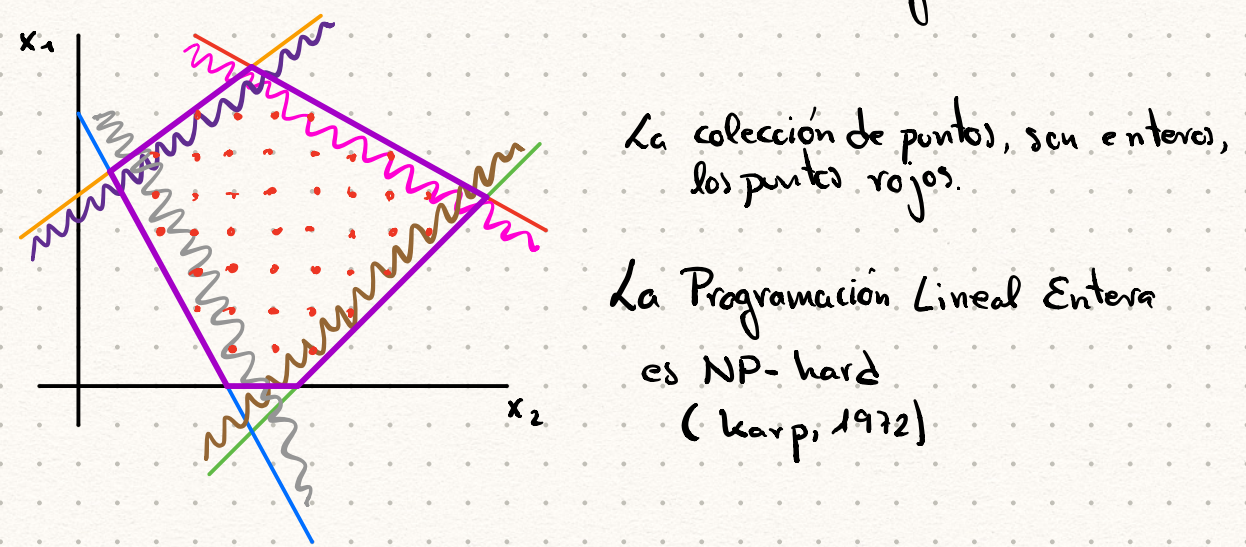
\includegraphics[scale=.3]{Untitled 18.png}}
\end{figure}
  \begin{itemize}
	\item Programación Entera Pura: \(x_i \in N^+_0; \forall i\) Todas las
    variables están afectadas por una restricción de integridad. 
	\begin{itemize}
		\item Pueden no tener solución, si no hay puntos enteros en las
		subregiones factibles.
	\end{itemize}
    
	\item
		Programación 0-1: \(x_i \in \{ 0, 1\}\)
  
	\item
      Programación Entera Mixta: Solo algunas variables de decisión
      tienen restricción de integridad.
  \end{itemize}
\pagebreak
  \subsection{Ramificación y Acotación en profundidad}

  Relajamos el problema, ignorando las restricciones de integridad, y
  vamos añadiendo las restricciones.

  Ramificamos una de las variables de decisión, creando dos
    subregiones factibles.
	\begin{figure}[H]
		\ffigbox[\FBwidth]
		{\caption{Ramificación}}
		{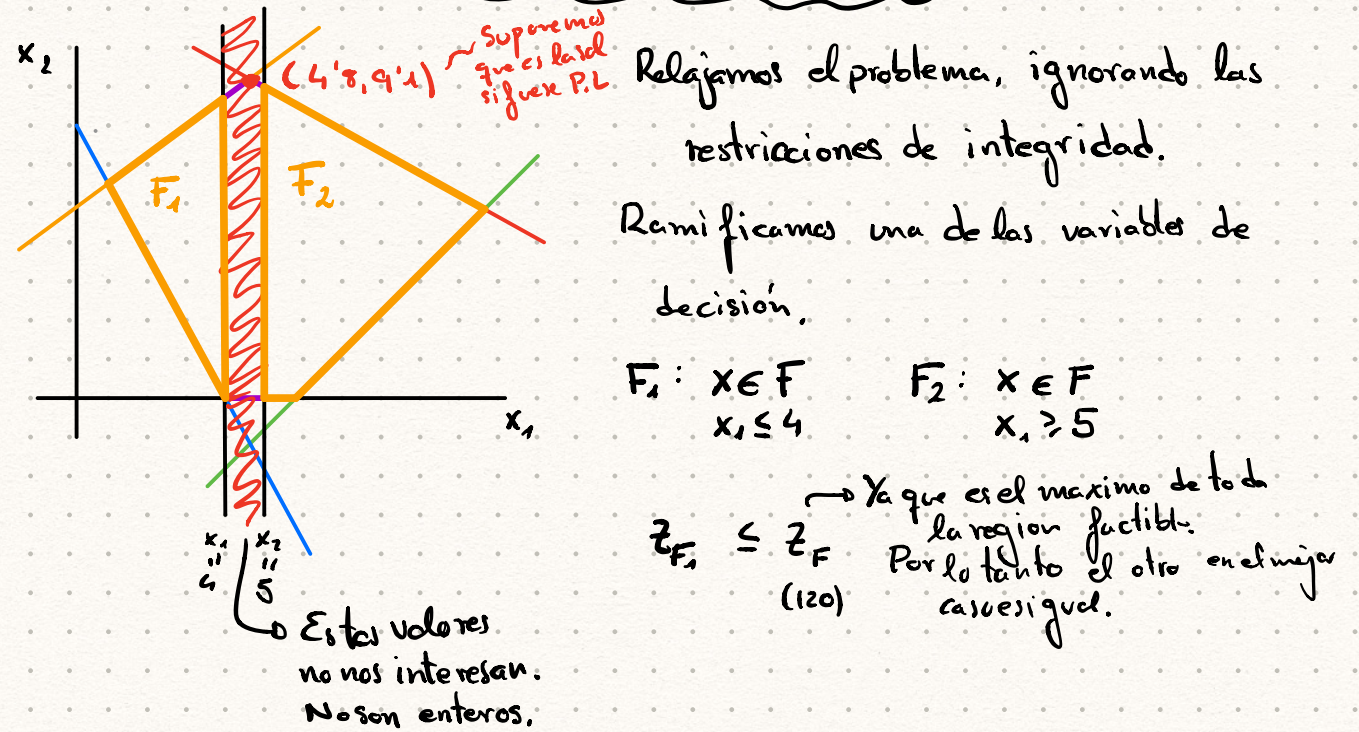
\includegraphics[scale=.25]{Untitled 19.png}}
	\end{figure}
	\vspace{-0.5cm}

  La solución óptima de las subregiones será peor o igual que la óptima
  relajada, \(z_S \leq z_F\).

    Dado el problema de Programación Lineal Entera:
	\vspace{-0.5cm}

	$$\max \space z= z(x)$$
	\vspace{-1cm}
    $$s.a \space x \in F; x_i \in N^+_0 \space \forall i$$

	Método:
	\vspace{-0.5cm}

    \begin{enumerate}

    \item
      $B ← -\infty$ o Valor negativo muy alto
    \item
      Resolver el Problema Relajado.

      \begin{itemize}
    	\vspace{-0.5cm}

      \item
        Si \(x* \in N^+_0\) entonces HALT
      \item
        En otro caso, ir al 3.
      \end{itemize}
    \item
      Aplicamos alguna regla de ramificación sobre una variable de
      decisión no entera: \(F_1, F_2\) (las llamaremos S, de subset)
    \item
      Determinar el valor de \(z_s\)
    \item
      Son nodos terminales:
	  \vspace{-0.5cm}

      \begin{itemize}
    
      \item
        \(S= \emptyset\) Infactible esa subregión, hacemos backtracking.
      \item
        \(z_s \leq B\) Peor que alguno de los terminales, hacemos
        backtracking
      \item
        \(x* \in N^+_0 , z_s > B\), entonces, \(B←z_s\)
      \end{itemize}
    \item
      Si todos los nodos son terminales, HALT, en otro caso, ir a 2.
    \end{enumerate}

	Ejemplo:

	\begin{figure}[H]
		\ffigbox[\FBwidth]
		{\caption{Ejemplo Programación Lineal Entera}}
		{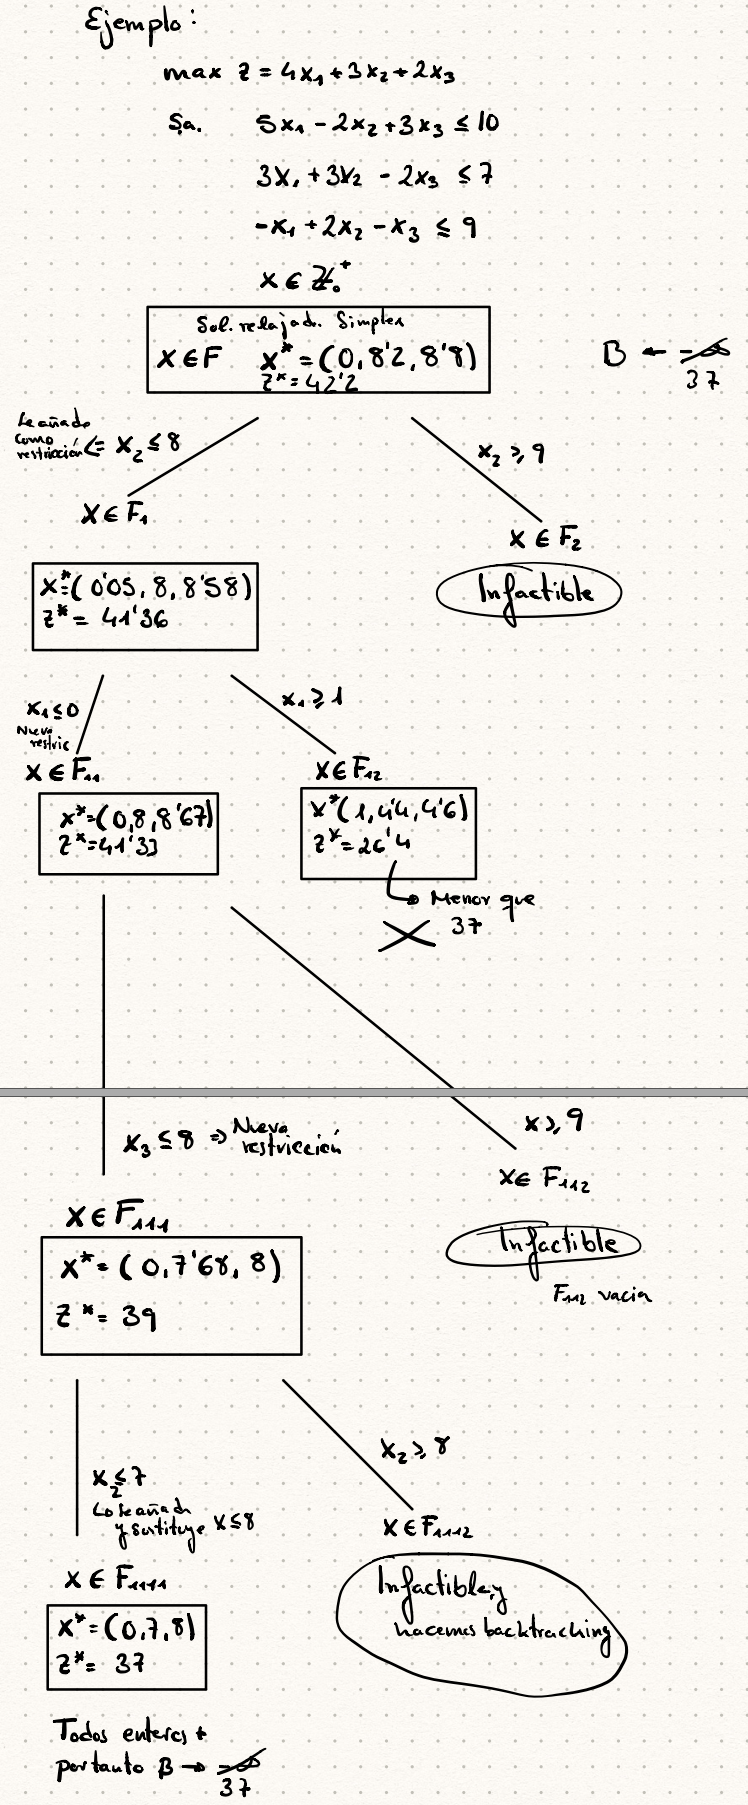
\includegraphics[scale=.32]{Untitled 20.png}}
	\end{figure}


\chapter{Tema 2 Programación Dinámica}

 
    Principio de Optimalidad: Una política óptima debe verificar que
    independientemente del estado inicial y decisiones iniciales, el
    resto de decisiones deben ser óptimas con respecto al estado que
    resulta de la primera decisión. (Bellman, 1957)

    \begin{itemize}
    \item
      Ejemplo que lo cumple: La ecuación de Bellman.
      \(V(x)= max_{a \in A} \{ f(x,a)+V(T(x,a))\}\)

      \begin{itemize}
    
      \item
        El coste de x, será el máximo evaluando todas las transiciones
        de: el coste de la acción a sobre más el coste del estado al que
        transiciona con la acción a sobre x.
      \end{itemize}
    \item
      Ejemplo que no lo cumple: Longest Path Problem - LPP.
    \end{itemize}

	Los problemas que verifican el principio de optimalidad también
    verifican la propiedad de Subestructura Óptima (Coman, 2009).

    \begin{itemize}
  
    \item
      Si es el camino optimo entre s y t, no habrá otro con menor coste.
      Además, para los nodos que se recorren continuar ese camino
      también será el camino optimo hasta t.
    \end{itemize}

	La programación dinámica sugiere:

    \begin{enumerate}  
    \item
      Descomponer el problema en subproblemas y caracterizar su
      estructura.
    \item
      Definir una expresión de recurrencia para calcular la solución
      óptima de los problemas.
    \item
      Derivar la solución óptima de cada problema. Calcular los valores
      de las soluciones óptimas de los subproblemas.
    \item
      Calcular la solución óptima del problema global.
    \end{enumerate}
\pagebreak
  Ejemplo programación dinámica en Coeficientes Binomiales:
  \begin{figure}[H]
	\ffigbox[\FBwidth]
	{\caption{Programación Dinamica I}}
	{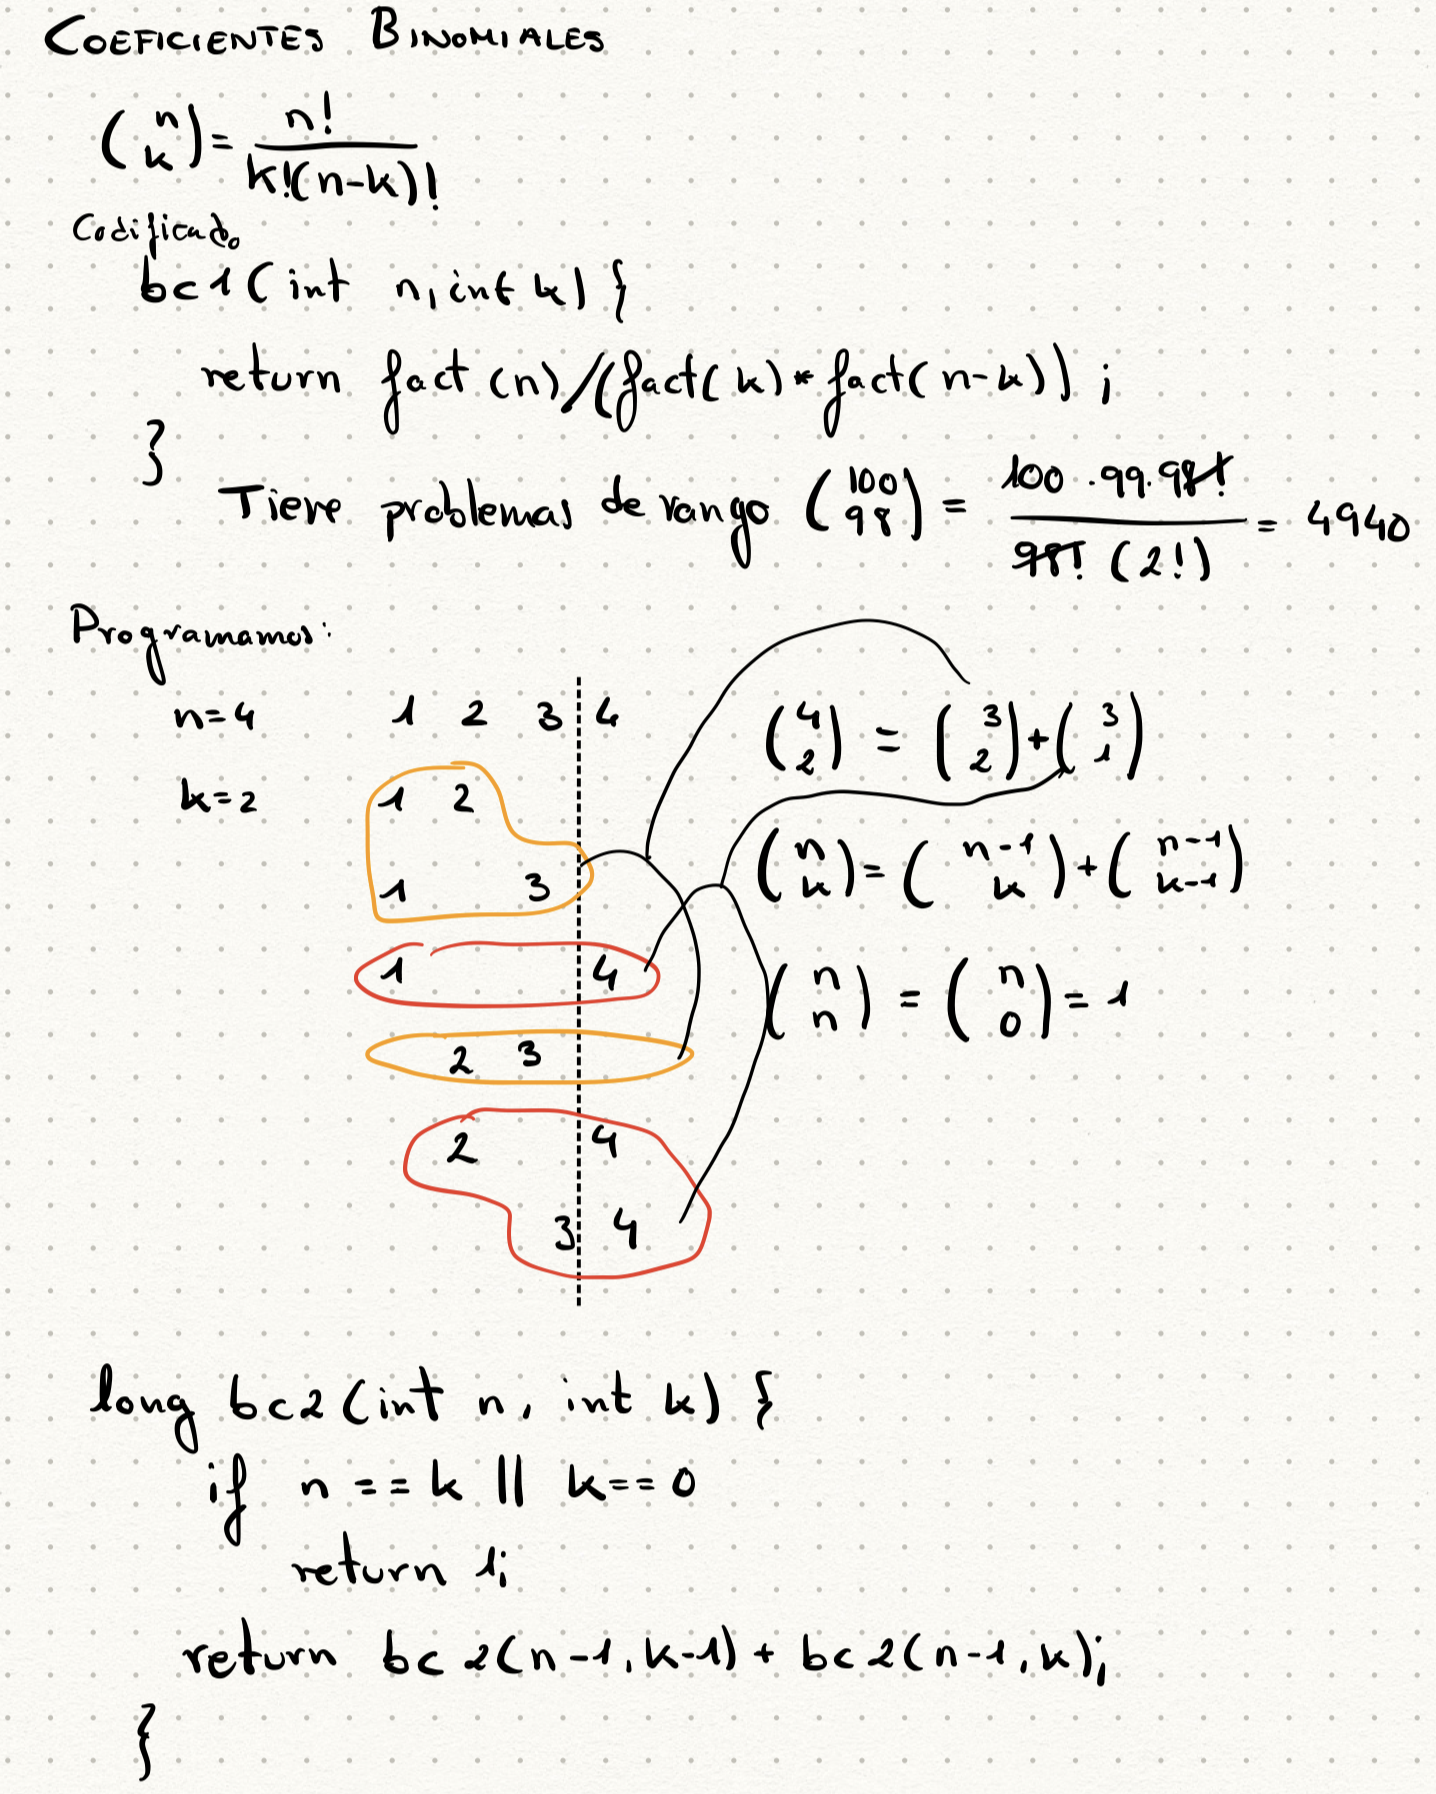
\includegraphics[scale=.32]{Untitled 23.png}}
\end{figure}
\begin{figure}[H]
	\ffigbox[\FBwidth]
	{\caption{Programación Dinamica II}}
	{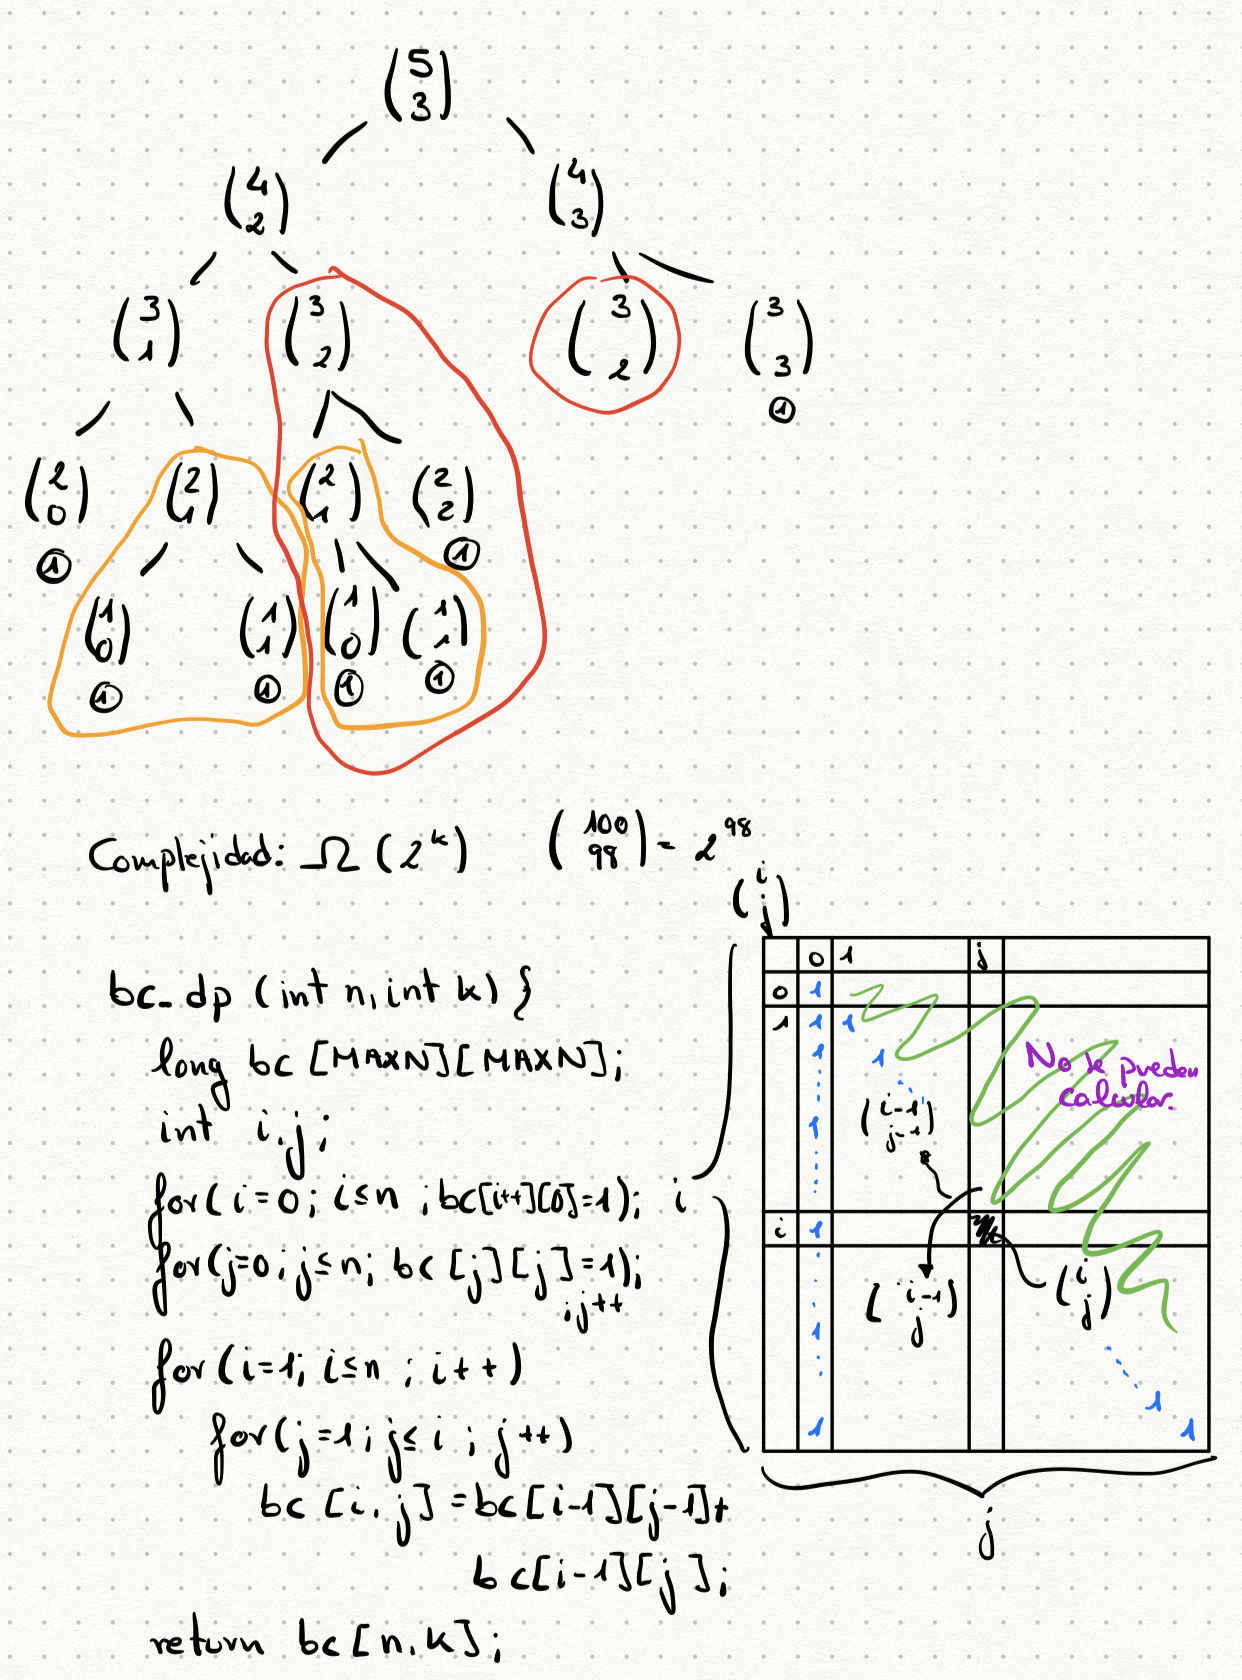
\includegraphics[scale=.32]{Untitled 24.png}}
\end{figure}
\pagebreak
\section{Single-Source Shortest-Path}

  
Dado un grafo \(G=(V,E)\) y una función de costes \(c: e → \mathbb{Z}\),
calcular el coste del camino optimo desde \(s \in V\) hasta todos los
demás vértices.

\subsection{Bellman-Ford-Moore (1958, 56, 57)}

El camino optimo entre dos puntos será: \(\min (d[e.v], d[e.u]+ e.c)\)
\begin{figure}[H]
	\ffigbox[\FBwidth]
	{\caption{Bellman-Ford-Moore}}
	{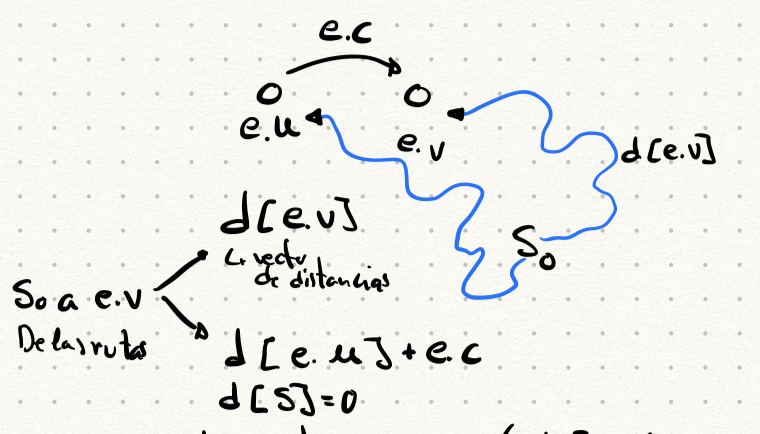
\includegraphics[scale=.32]{Untitled 25.png}}
\end{figure}
\begin{itemize}
\item
  e.u = origen
\item
  e.v = destino
\item
  e.c = coste del arco entre u y v
\item
    Lo que quiere decir, que escogemos el menor entre, el coste de ir al
    destino ya calculado o el coste de ir a otro punto y coger desde
    este un arco al destino.
\end{itemize}
\begin{lstlisting}[language=Python]
def bellmanFordMoore (V,E,s):
	for v in V:
		if V==s: d[v]=0
		else: d[v]= +infinito
	for i in range(len(V)-1):
		for e in E:
			d[e.v]= min(d[e.v], d[e.u]+e.c)
	for e in E:
		if d[e.u]+e.c<d[e.v]
			raise(...) #Ciclos negativos
\end{lstlisting}

\pagebreak
Ejemplo
\begin{figure}[H]
	\ffigbox[\FBwidth]
	{\caption{Ejemplo Bellman-Ford-Moore}}
	{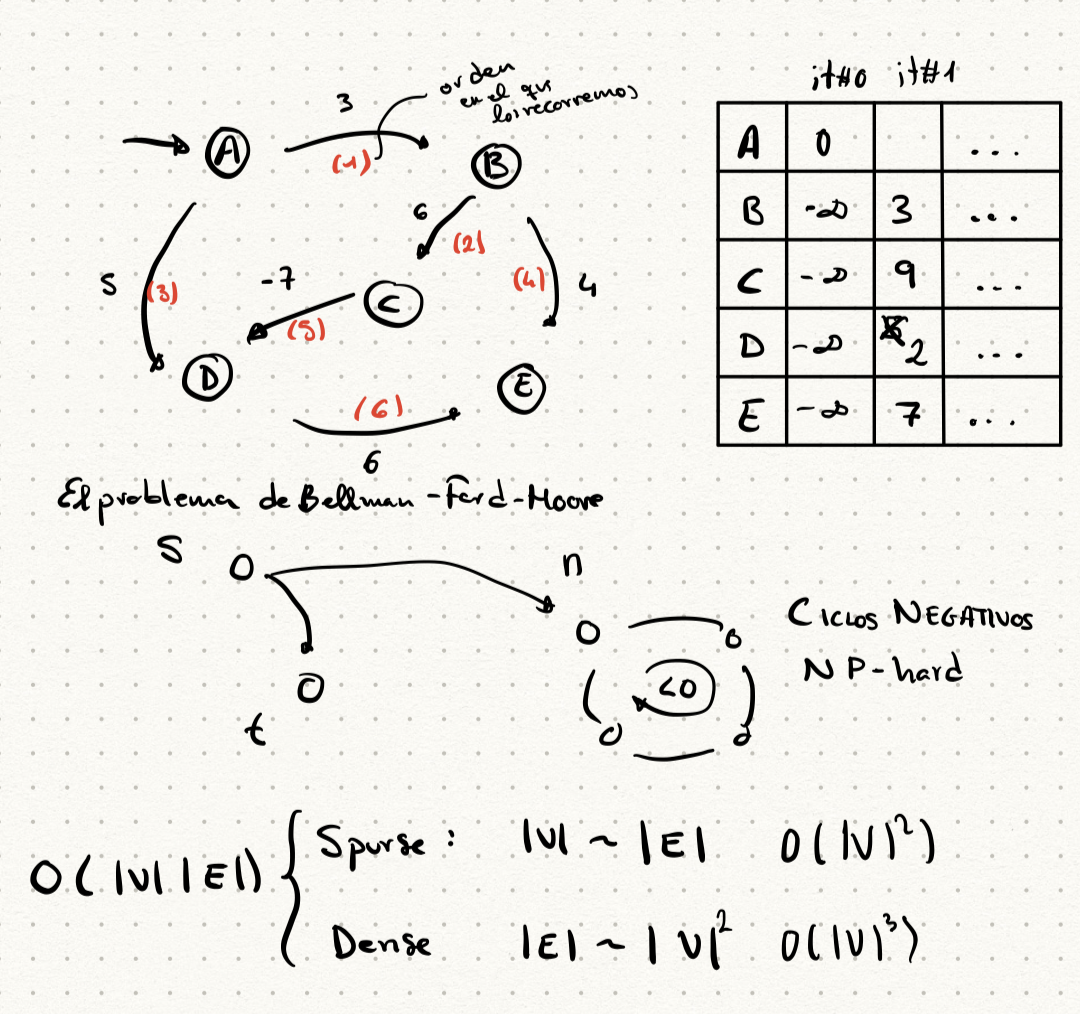
\includegraphics[scale=.3]{Untitled 26.png}}
\end{figure}
Complejidad:

\begin{itemize}

\item Spurse: \(O(|V|^2)\)
\item Dense: \(O(|V|^3)\)
\end{itemize}


\section{All Pairs Shortest-Path}

Dado un grafo \(G=(V,E)\) y una función de costes \(c: e → \mathbb{Z}\),
el coste del camino más corto entre cada par de vértices.

\begin{itemize}
\item Aplicando Bellman-Ford-Moore, la complejidad es \(O(|V|^3)-O(|V|^4)\)
\end{itemize}

\subsection{Floyd-Warshall}

En cada iteración vamos añadiendo un vértice más que podemos visitar.

\begin{itemize}
	\item $D_{ij}^{(k} = \min \{ D_{ij}^{(k-1}, D_{ik}^{(k-1}+D_{kj}^{(k-1} \}$ k son los vértices auxiliares que vamos añadiendo.
	\item $D_{ii}^{(0} =0$
	\item $D_{ij}^{(0}= c(e(i,j))$ si hay arco entre i y j, si no es $D_{ij}^{(0}= + \infty$
\end{itemize}
     

Algoritmo: 
\begin{itemize}
	\item Partimos de una matriz con los costes a los vértices
	\item Ahora en cada
	iteración vamos añadiendo un vértice, k, que podemos usar como
	intermediario.
	\begin{itemize}
		\item En cada una de esas iteraciones evaluamos todos los
		vértices con todos los vértices, ir de i a j.
		
		Para cada par evaluado
		nos quedamos con el menor entre, el coste de ir de uno al otro previo,
		dij, o el coste de ir del origen al vértice que hemos añadido más el
		cose de ir desde el vértice añadido al destino, dik+dkj.
	\end{itemize}
	
\end{itemize}

\begin{lstlisting}[language=Python]
def floydwarshall:
	for v in V:
		d[v][v]=0
	for e in E:
		d[e.u][e.v]=e.c
	for k in V:
		for i in V: 
			for j in V:
				d[i][j]= min(d[i][j],d[i][k]+d[k][j])
\end{lstlisting}

  Diagrama:
  \begin{figure}[H]
	\ffigbox[\FBwidth]
	{\caption{Floyd-Warshall:}}
	{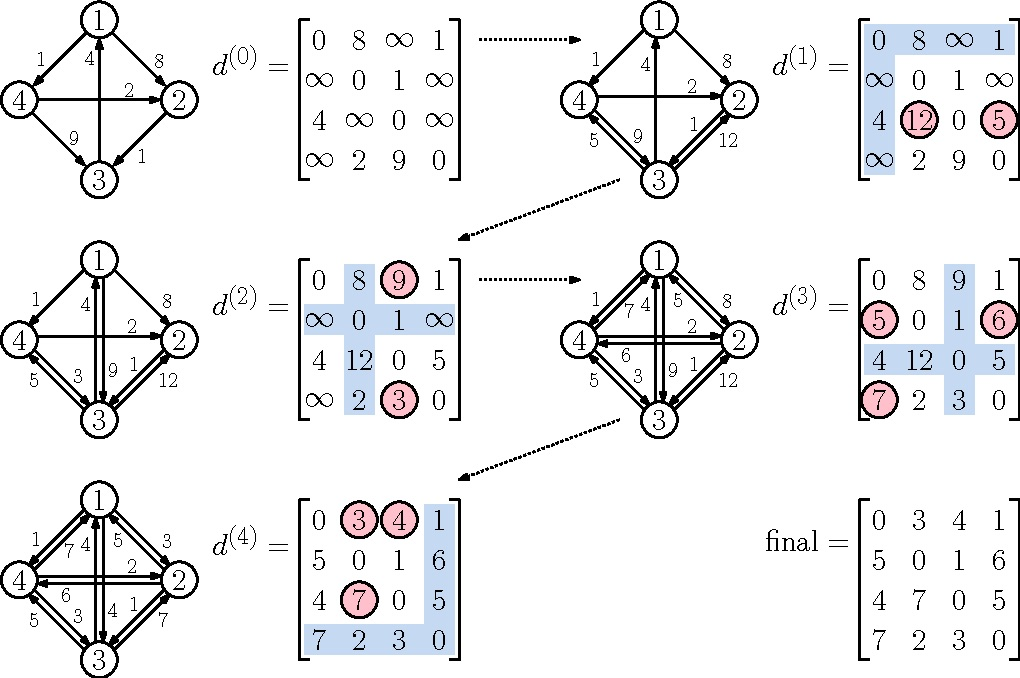
\includegraphics[scale=.3]{2A6EA3F5-5BA5-4FDB-9D83-EB572452B3AB.jpeg}}
\end{figure}
  \begin{itemize}
  \item Complejidad: \(O(|V|^3)\)
  \end{itemize}
  

\chapter{Tema 3 Satisfabilidad}

  \begin{enumerate}

  \item
    Una formula está en Forma Normal Conjuntiva si y solo si:
    \(F \equiv \bigwedge_{i=1}^{n} \zeta_i= \bigwedge_{i=1}^{n} (\bigvee_{j=1}^{\left | \zeta_i \right |} \ell_i)\)
	\vspace{-0.5cm}
    \begin{itemize}
    \item Ejemplo:
      \((x_1 \vee \overline{x_2})\wedge (\overline{x_1} \vee \overline{x_2} \vee x_3)\)

      \begin{itemize}
    
      \item
        3 variables: \(x_1, x_2, x_3\)
      \item
        4 literales: \(x_1,\overline{x_1}, \overline{x_2}, x_3\)
      \item
        2 cláusulas:
        \((x_1 \vee \overline{x_2}),(\overline{x_1} \vee \overline{x_2} \vee x_3)\)
      \end{itemize}
    \end{itemize}
  \item
    Las variables x pueden estar afirmadas \((x)\) o negadas
    \((\overline{x})\) , y se denomina literal a la asociación de una
    variable y su signo.
  \item
    Un literal \(\ell\) es puro si y solo si \(\overline{\ell}\) no
    aparece en \(F\) (\(\overline{\ell} \notin F\))

    \begin{itemize}
  
    \item
      Ejemplo: \(x_1\) y \(\overline{x_1}\) no son literales puros
    \end{itemize}
  \item
    Un modelo M consiste en una asignación de las constantes
    proposicionales (\(\perp falso,\top verdadero\) ) a todos o algunas
    de las variables de \(F\) que le satisfagan, \(M \models F\)
  \end{enumerate}

  \begin{itemize}

  \item
    El problema de SAT (Satisfabilidad) consiste en encontrar al menos
    un modelo \(M \models F\), o probar que no existe ninguno. (K-SAT es
    NP-complete \(K \geq 3\))
  \end{itemize}
  \vspace{-0.5cm}
\section{Método de Resolución}
\vspace{-0.5cm}
    $$Res(F,x)\left\{\begin{matrix}  
		F &si&x\notin F \\  
		F-x &si& x \text{ es un literal puro en } F \\  
		(c_1 \vee c_2) &si& \begin{matrix}  (x \vee c_1) \in F\\  
		(\overline{x} \vee c_1) \in F  \end{matrix}  \end{matrix}\right.$$

	Tautología: Toma el valor cierto siempre.
	\vspace{-0.5cm}

    
	$$F \equiv (x_1 \vee \overline{x_2})\wedge (\overline{x_1} \vee x_2)$$
	$$Res(F,x_1)= \emptyset \space SAT$$

	Contradicción: Nunca será cierta.
	\vspace{-0.5cm}

	$$F \equiv (x_1)\wedge (\overline{x_1})$$
	$$Res(F,x_1)= \emptyset \vee \emptyset = \{ \emptyset \} \space UNSAT$$

	  
	Si resulta la cláusula vacía, \(\{ \emptyset \}\), UNSAT

	
  Si resulta la conjunto vacía, \(\emptyset\), SAT

  
  
    Ejemplos:
	\begin{figure}[H]
		\ffigbox[\FBwidth]
		{\caption{Resolución FNC}}
		{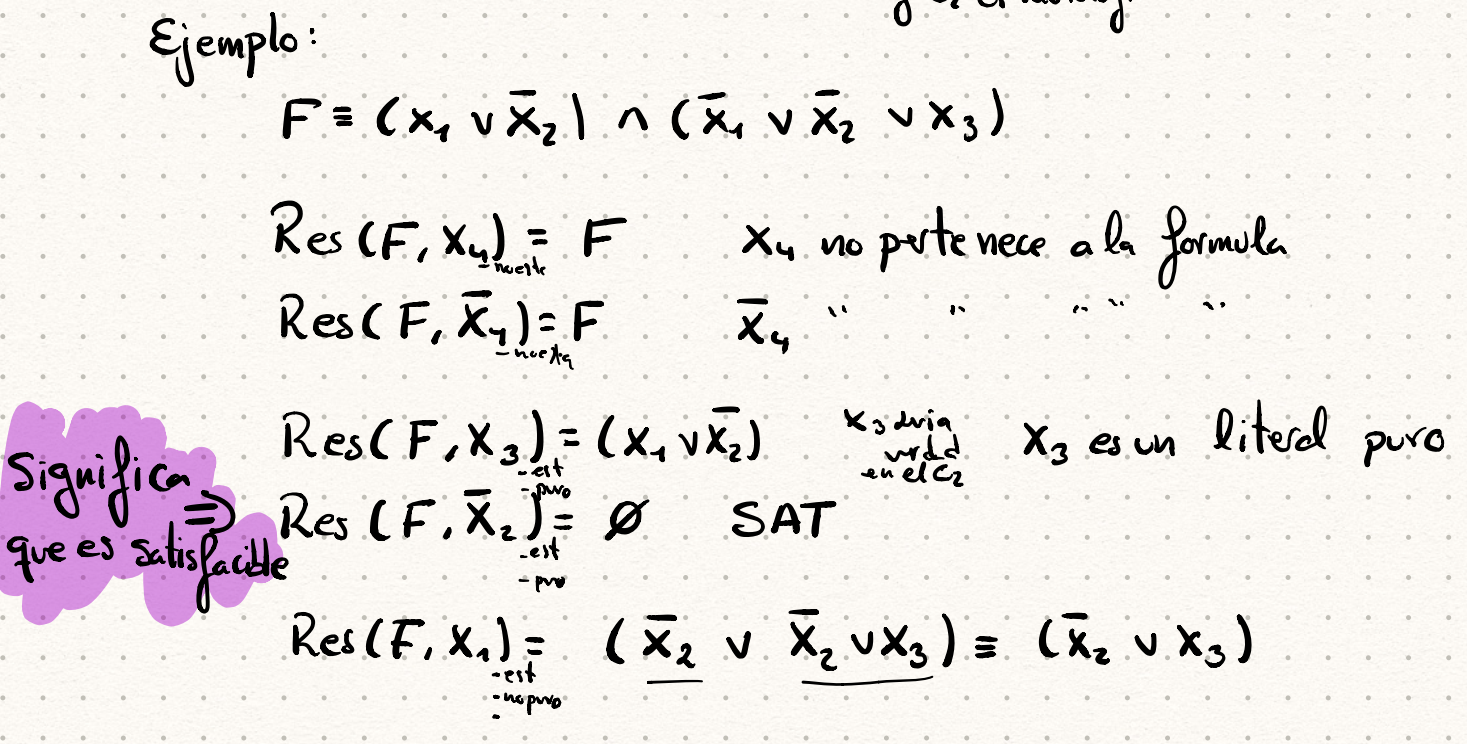
\includegraphics[scale=.2]{Untitled 29.png}}
	\end{figure}
	El modelo de resolución reduce el número de variables, pero no
    necesariamente el número de cláusulas será \(\frac {n^2} {4}\)

	
  El método de resolución no genera modelos, aunque preserva la
  identidad lógica.


  
    Ejemplo UNSAT
	\begin{figure}[H]
		\ffigbox[\FBwidth]
		{\caption{Ejemplo UNSAT}}
		{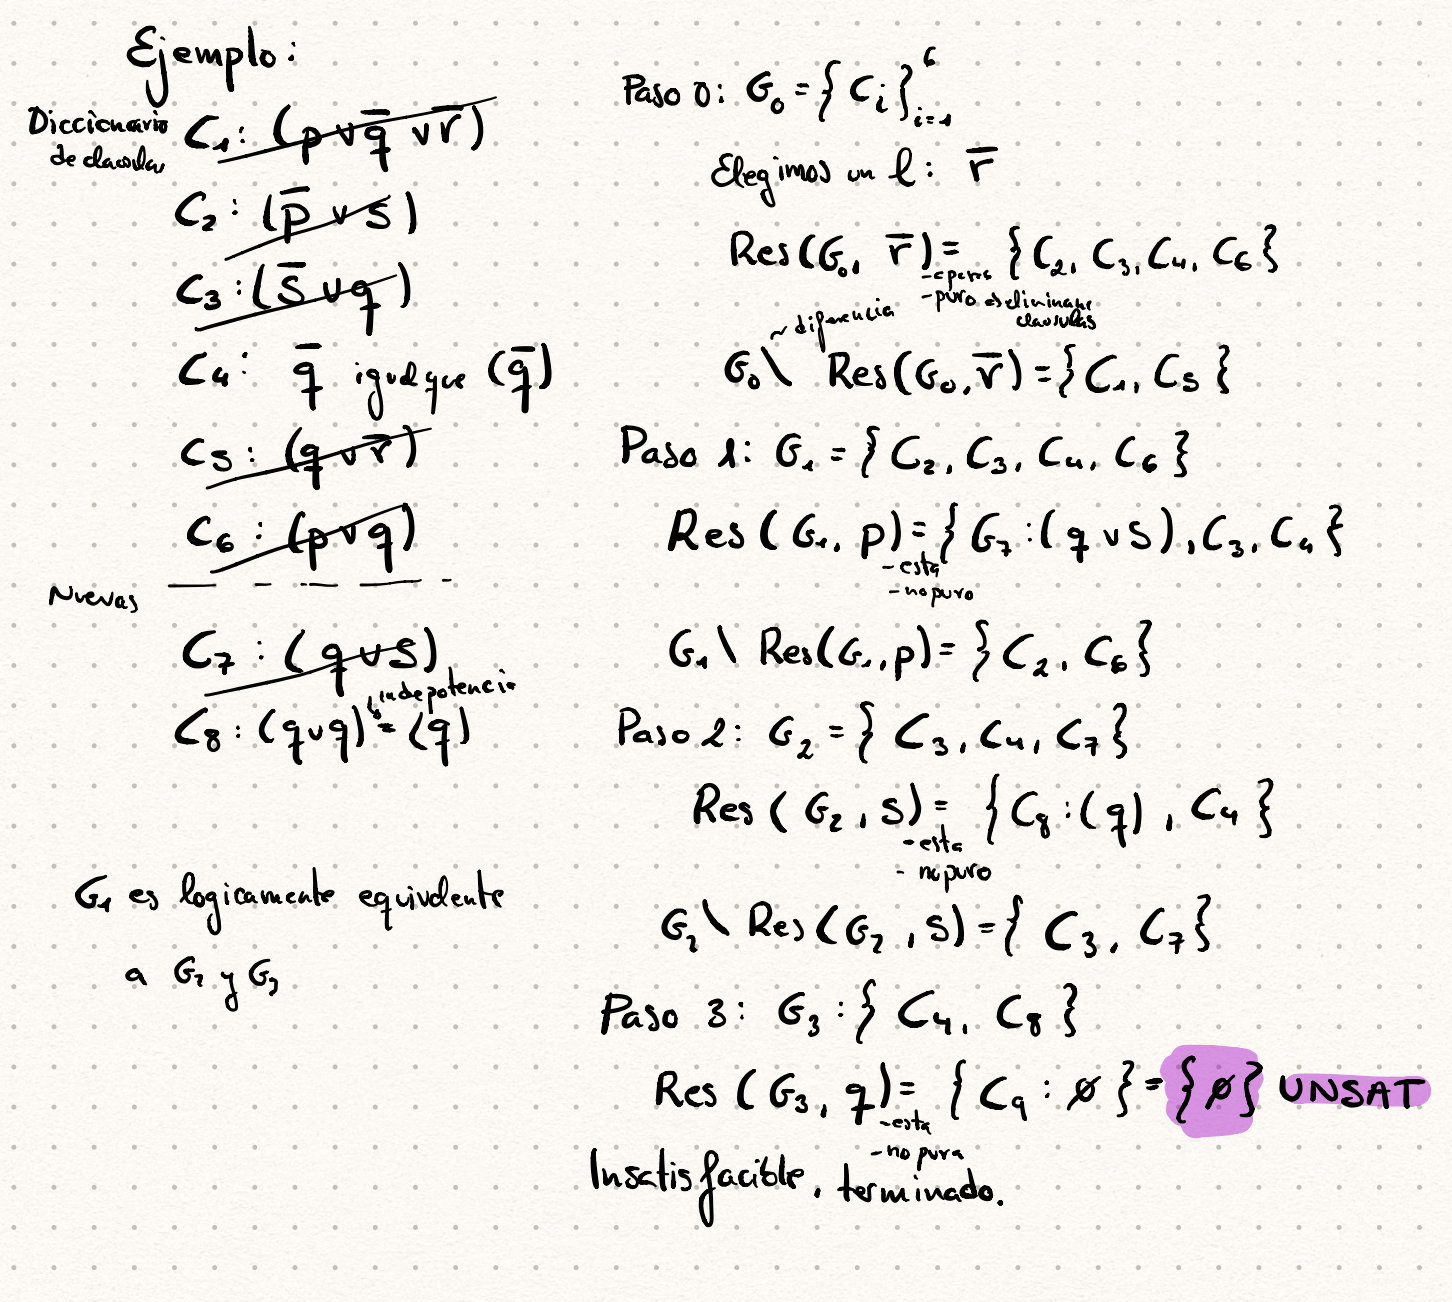
\includegraphics[scale=.25]{Untitled 31.png}}
	\end{figure}
	\pagebreak
	Ejemplo SAT
	\begin{figure}[H]
		\ffigbox[\FBwidth]
		{\caption{Ejemplo SAT}}
		{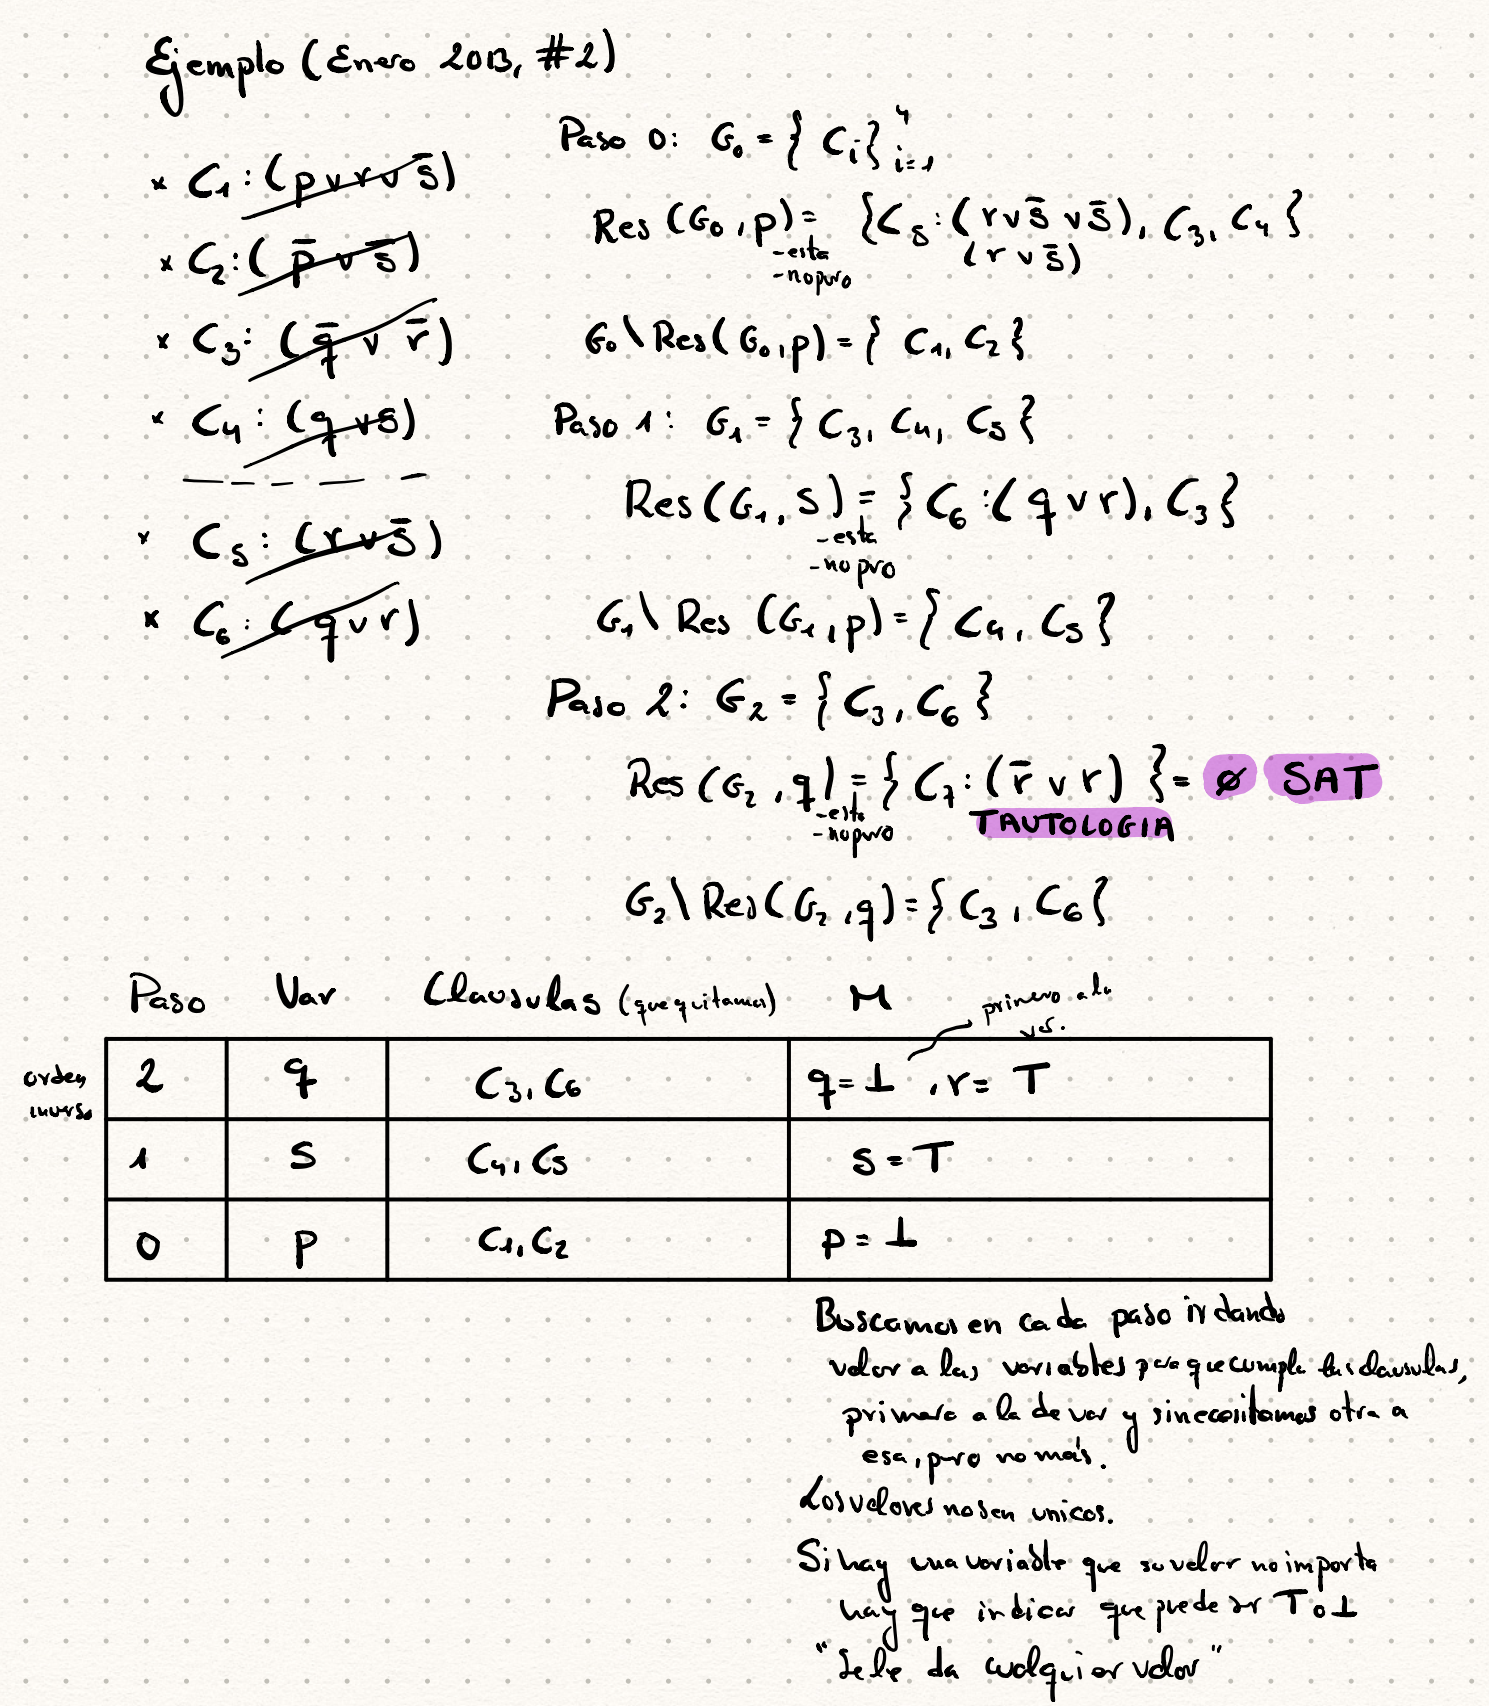
\includegraphics[scale=.28]{Untitled 32.png}}
	\end{figure}
	\pagebreak
\section{Algoritmos}
\subsection{Davis-Putnam (DP)}

  \begin{enumerate}

  \item
    Selección de un literal \(\ell \in F\) (empezando por los puros)
  \item
    Aplicar \(Res(F,\ell)\) y anotando la variable usada y las cláusulas
    involucradas.

    \begin{itemize}
  
    \item
      Si creamos cláusulas que son Tautologías no las ponemos, se
      satisfacen directamente.
    \end{itemize}
  \item
    Si resulta $\{ \emptyset \}$, F es UNSAT. Entonces HALT

    \begin{itemize}
  
    \item
      Cuando hay que juntar cláusulas y la misma variable, pero cada una
      con un signo y se unen los vacíos.
    \end{itemize}
  \item
    Si resulta \(\emptyset\), F es SAT. Ir a 6.

    \begin{itemize}
  
    \item
      Cuando queda una sola cláusula con un único literal, por lo que se
      elimina en la siguiente.
    \item
      Cuando al juntar literales no puros queda una tautología.
    \end{itemize}
  \item
    En otro caso, ir a 1.
  \item
    Considerar las variables usables y las cláusulas involucradas en
    orden inverso, y asignar los valores \(\perp\) y \(\top\) a las
    variables usadas (y otras si hiciera falta) para satisfacer esas
    clausulas.
  \end{enumerate}

    Del 1-5 es la Fase I, es de progreso.

	La 6 es la Fase II, de regresión.
\pagebreak
    Ejemplo
	\begin{figure}[H]
		\ffigbox[\FBwidth]
		{\caption{Davis-Putnam}}
		{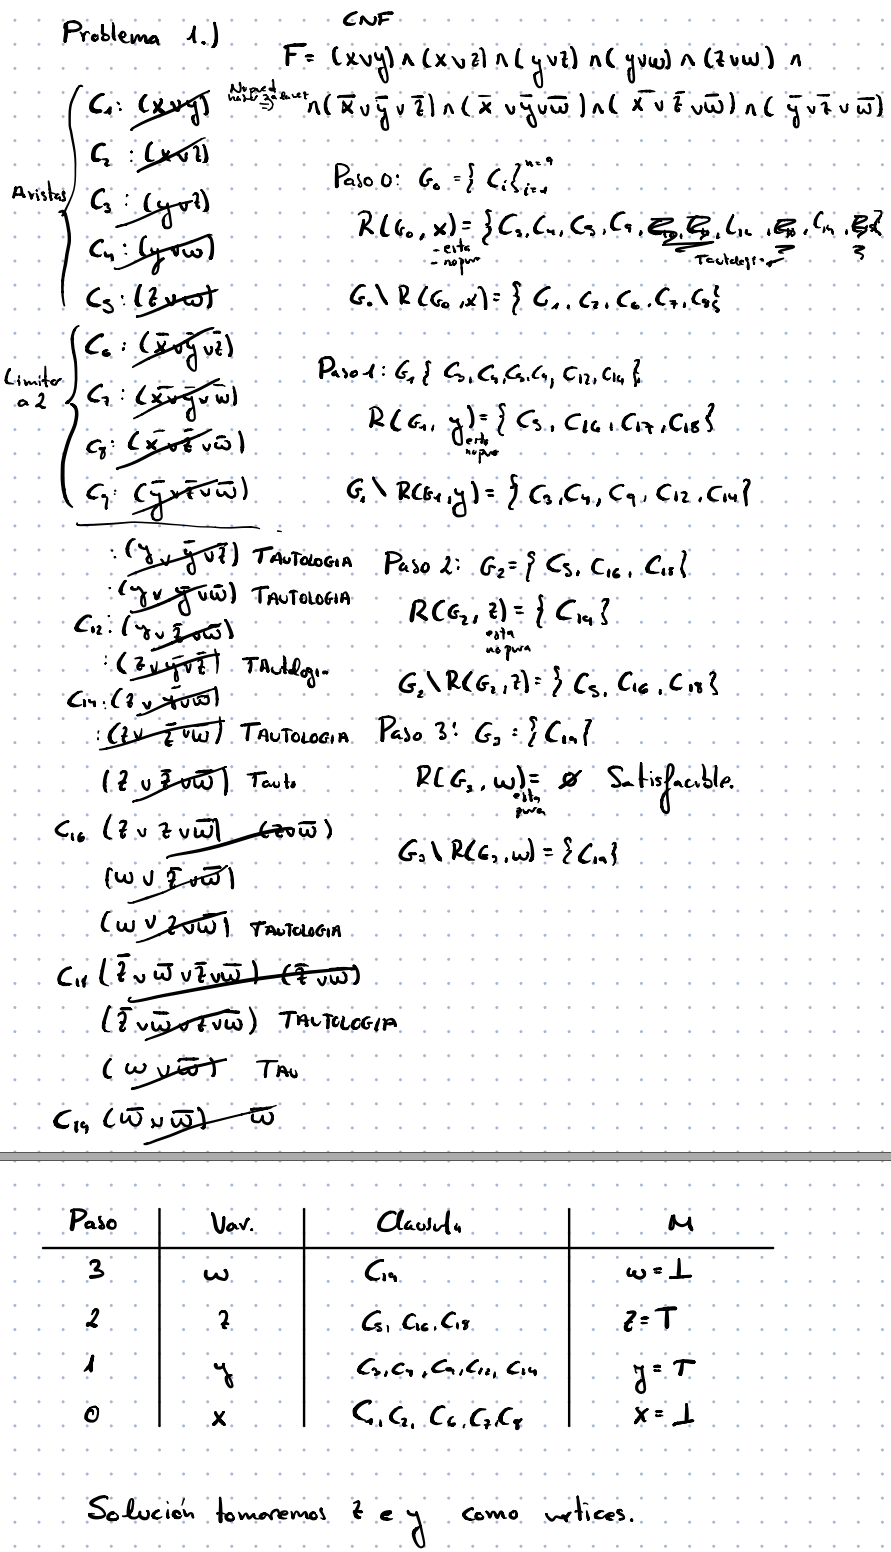
\includegraphics[scale=.4]{Untitled 33.png}}
	\end{figure}

	
\subsection{Davis-Putnam-Logemann-Loveland (DPLL)}

  \begin{enumerate}
  \def\labelenumi{\arabic{enumi}.}

  \item
    Resolución unitaria: Resolución en la que una, al menos de las
    cláusulas padre es unitaria.
  \item
    Sea F una CNF y \(\ell \in F\). Si F es SAT entonces
    \(F \cup \{ \ell \}\) es SAT o \(F \cup \{ \overline{\ell} \}\) es
    SAT.
  \end{enumerate}

  \begin{itemize}
  \item
    Se denomina reducción de una formula F por un modelo parcial v a la
    formula resultante \(F_v = Red(F, v\)) en la que se han propagado
    las asignaciones de v

    \begin{itemize}
  
    \item
      Si el modelo es completo y resulta el conjunto vacío, entonces la
      formula F es satisfacible y el modelo v lo valida
    \end{itemize}
  \end{itemize}

  Ejemplo
  \begin{figure}[H]
	\ffigbox[\FBwidth]
	{\caption{Davis-Putnam-Logemann-Loveland}}
	{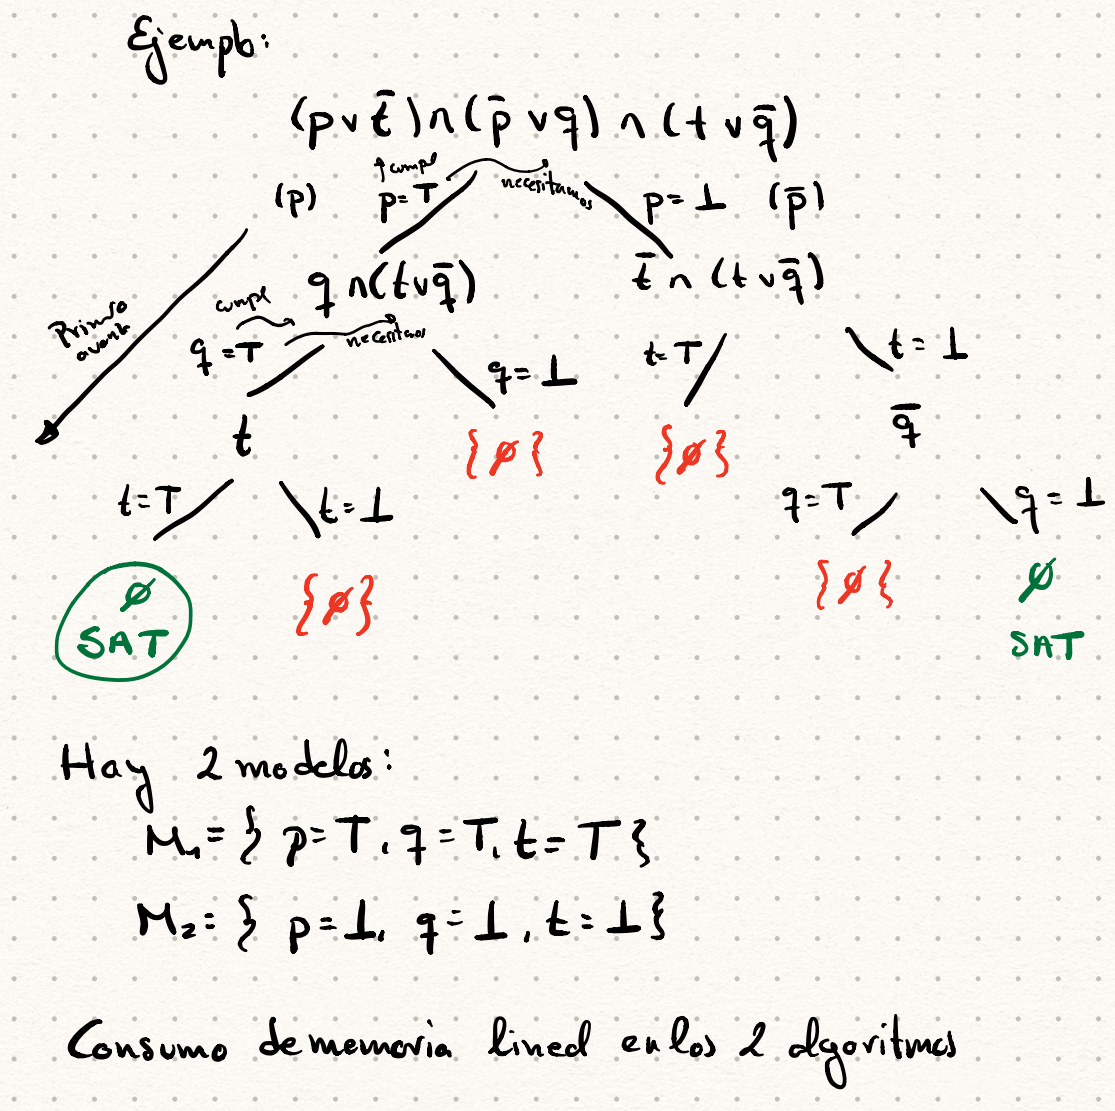
\includegraphics[scale=.35]{Untitled 34.png}}
\end{figure}

\subsection{CSP - Procedimiento de Satisfacción de Restricciones}

  \begin{enumerate}
  \def\labelenumi{\arabic{enumi}.}
  \item
    Una Red De Restricciones R consiste en un conjunto de variables
    \(X=\{ X_i \}^n_{i=1}\) definidas sobre un dominio
    \(D=\{ D_i \}^h_{j=1}\) que contienen los posibles valores de cada
    variable \(D_i=\{ V_1^{(i}, V_2^{(i}, ..., V_k^{(i} \}\) y un
    conjunto de restricciones \(C=\{ C_i \}^m_{n=1}\).

    \begin{itemize}
  
    \item
      \(R = (X, D, C)\)
    \end{itemize}
  \end{enumerate}

  
\begin{enumerate}
\def\labelenumi{\arabic{enumi}.}
\setcounter{enumi}{1}

\item
  Una restricciones \(C_i\) consiste en una relación (bidireccional
  típicamente) definida sobre un subconjunto de variables
  \(S \subseteq X\), que denota todas las asignaciones simultáneamente
  legales.

  \item
    Problema de las n reinas.
	\begin{figure}[H]
		\ffigbox[\FBwidth]
		{\caption{Problema de las n reinas}}
		{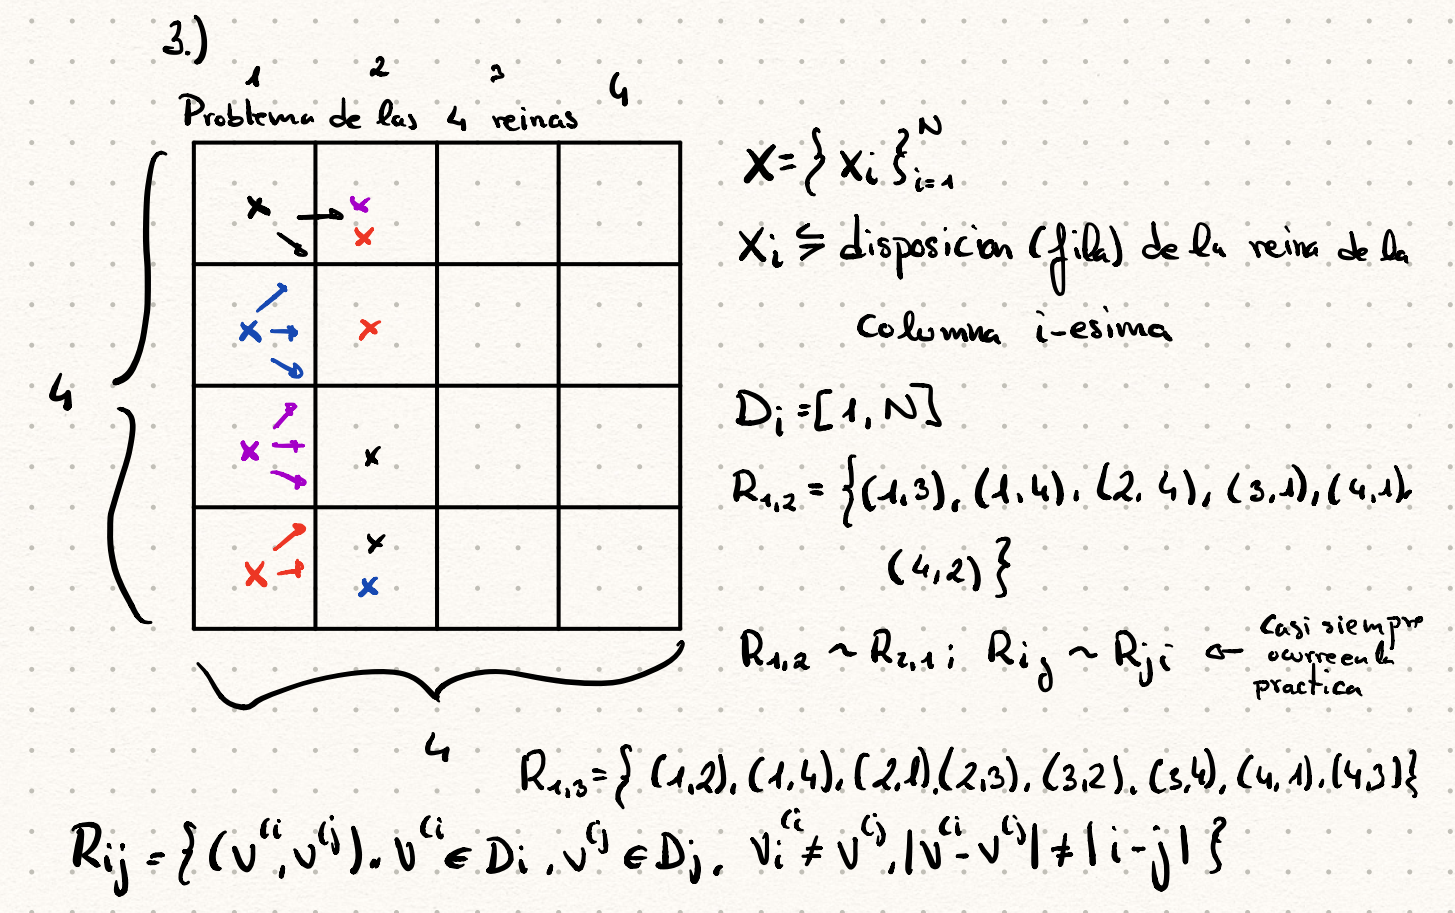
\includegraphics[scale=.25]{Untitled 35.png}}
	\end{figure}
  \item
    Una instanciación de un subconjunto de variables \(S \subseteq X\)
    consiste en una asignación de valores de los dominios de las
    variables en S que sea consistente con las restricciones.

    \begin{enumerate}
  
    \item
      \(S \subset X\): instanciación parcial.
	  \item
    \(S = X\): instanciación total.
    \end{enumerate}
  

    \begin{itemize}
  
    \item
      No siempre es posible extender una instanciación parcial a otra
      total.

	\item
	  Objetivo: Dada una red de restricciones \(R(X, D, C)\) encontrar una
	  instanciación total que sea compatible con todas las restricciones en
	  \(C\), si existe alguna, en otro caso, salir con una instanciación
	  vacía.
    \end{itemize}

	\item
    Una red de restricciones \(R(C, D, C)\) puede representarse como un
    grafo donde los vértices representan X, y hay un arco entre los
    vértices \(x_i\) y \(x_j\) si \(R_{ij} \neq \emptyset\)
	\begin{figure}[H]
		\ffigbox[\FBwidth]
		{\caption{Red de restricciones}}
		{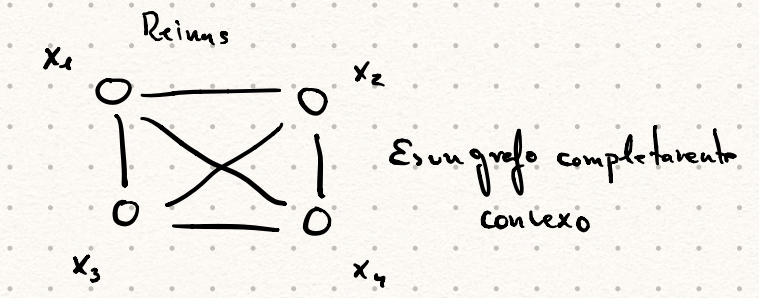
\includegraphics[scale=.35]{Untitled 36.png}}
	\end{figure}
\end{enumerate}


\subsection{Arco-Consistencia}

Una variable \(x_i\) es arco-consistente con otra variable \(x_j\) si
  y solo si para cada \(a_i \in D_i\), existe otro valor
  \(a_j \in D_j\),, \((a_i,a_j) \in R_{ij}\)

    Arco-consistencia es Direccional.
	\begin{figure}[H]
		\ffigbox[\FBwidth]
		{\caption{Arco-consistencia I}}
		{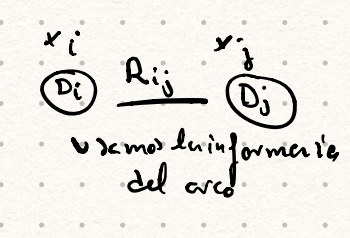
\includegraphics[scale=.5]{Untitled 37.png}}
	\end{figure}
	\begin{figure}[H]
		\ffigbox[\FBwidth]
		{\caption{Arco-consistencia II}}
		{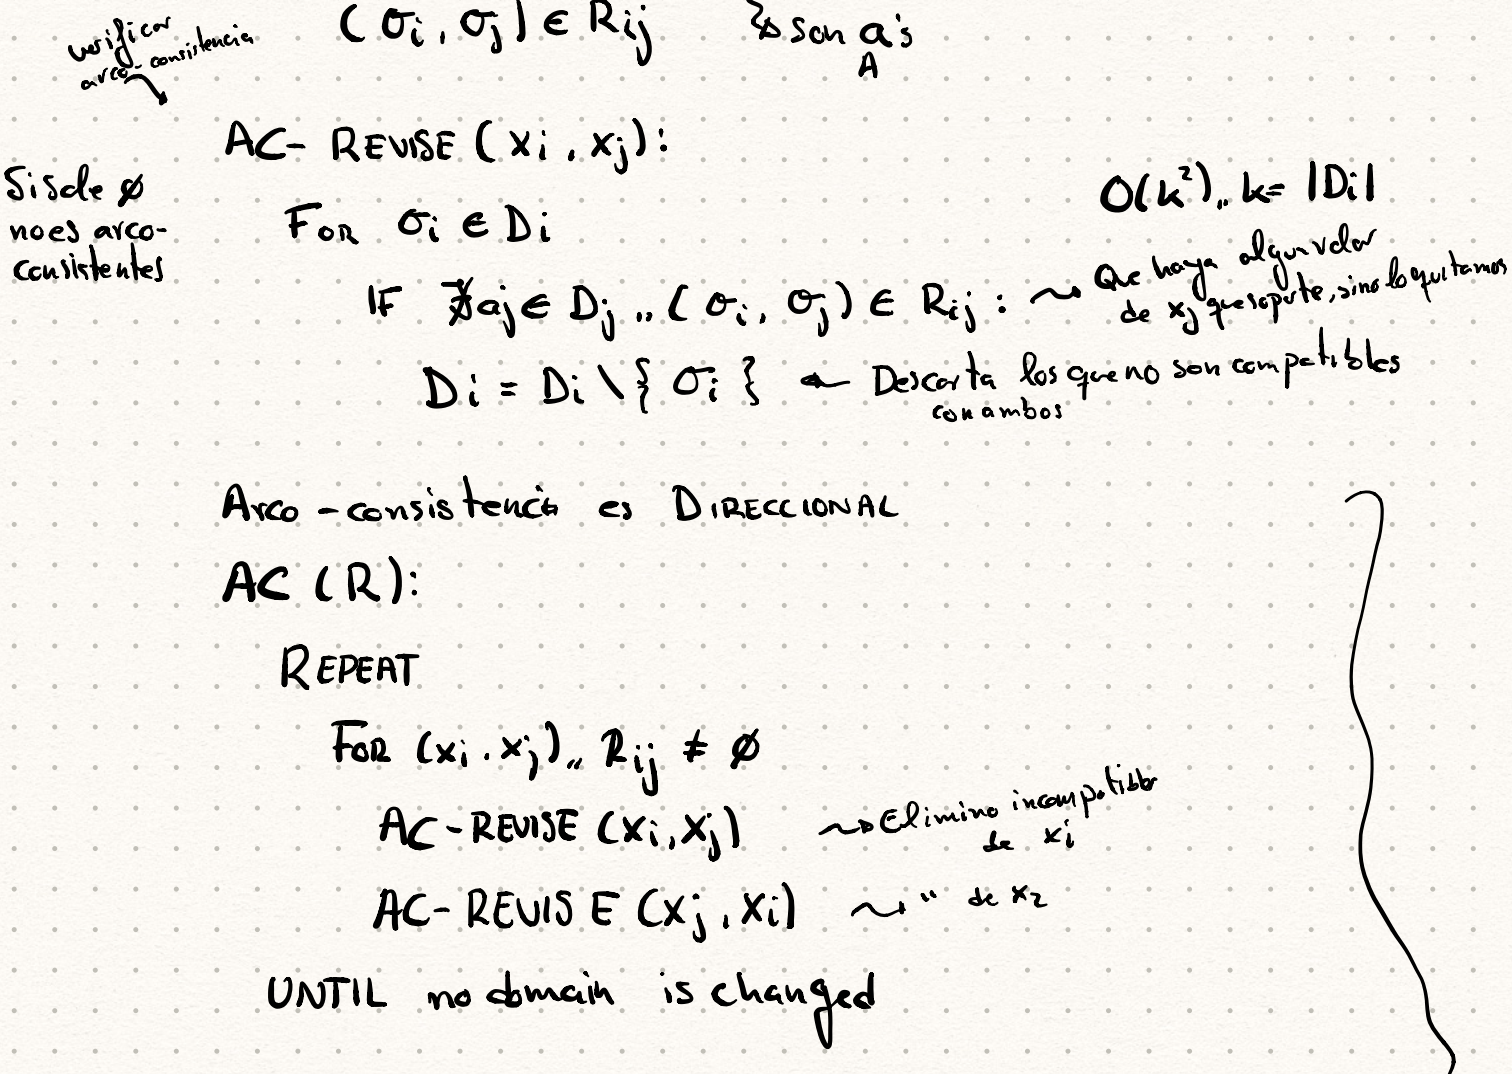
\includegraphics[scale=.2]{Untitled 38.png}}
	\end{figure}
	\pagebreak
	La arco-consistencia NO sirve para verificar la consistencia global.
    Ya que los arcos lo verifican para ese par solamente.
	\begin{figure}[H]
		\ffigbox[\FBwidth]
		{\caption{Arco-consistencia III}}
		{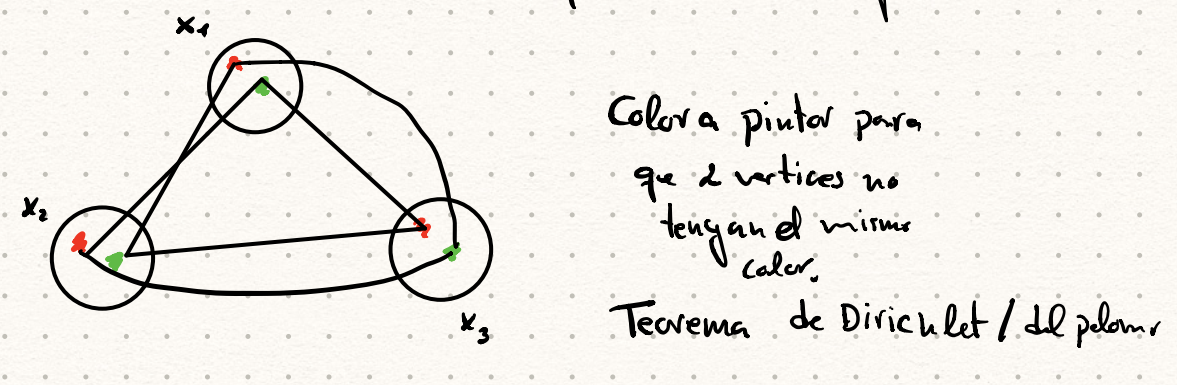
\includegraphics[scale=.35]{Untitled 39.png}}
	\end{figure}

	
\subsection{Camino-Consistencia}


    La variable \(x_i\) es camino-consistente con \(x_j\) con respecto
    de \(x_k\) si y solo si para cada \((a_i,a_j) \in R_{ij}\) y
    \(a_k \in D_k\),, \((a_i,a_k) \in R_{ik}\) y
    \((a_j,a_k) \in R_{jk}\).

    \begin{itemize}
    \item
      La camino-consistencia NO es direccional.
	  \begin{figure}[H]
		\ffigbox[\FBwidth]
		{\caption{Camino-Consistencia I}}
		{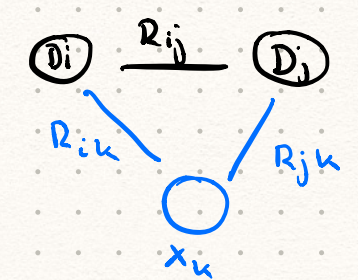
\includegraphics[scale=.42]{Untitled 40.png}}
	\end{figure}
	\pagebreak
    \item
      La camino-consistencia tampoco sirve para verificar la
      consistencia global. (por ejemplo, si aumenta a 4)
	  \begin{figure}[H]
		\ffigbox[\FBwidth]
		{\caption{Camino-Consistencia II}}
		{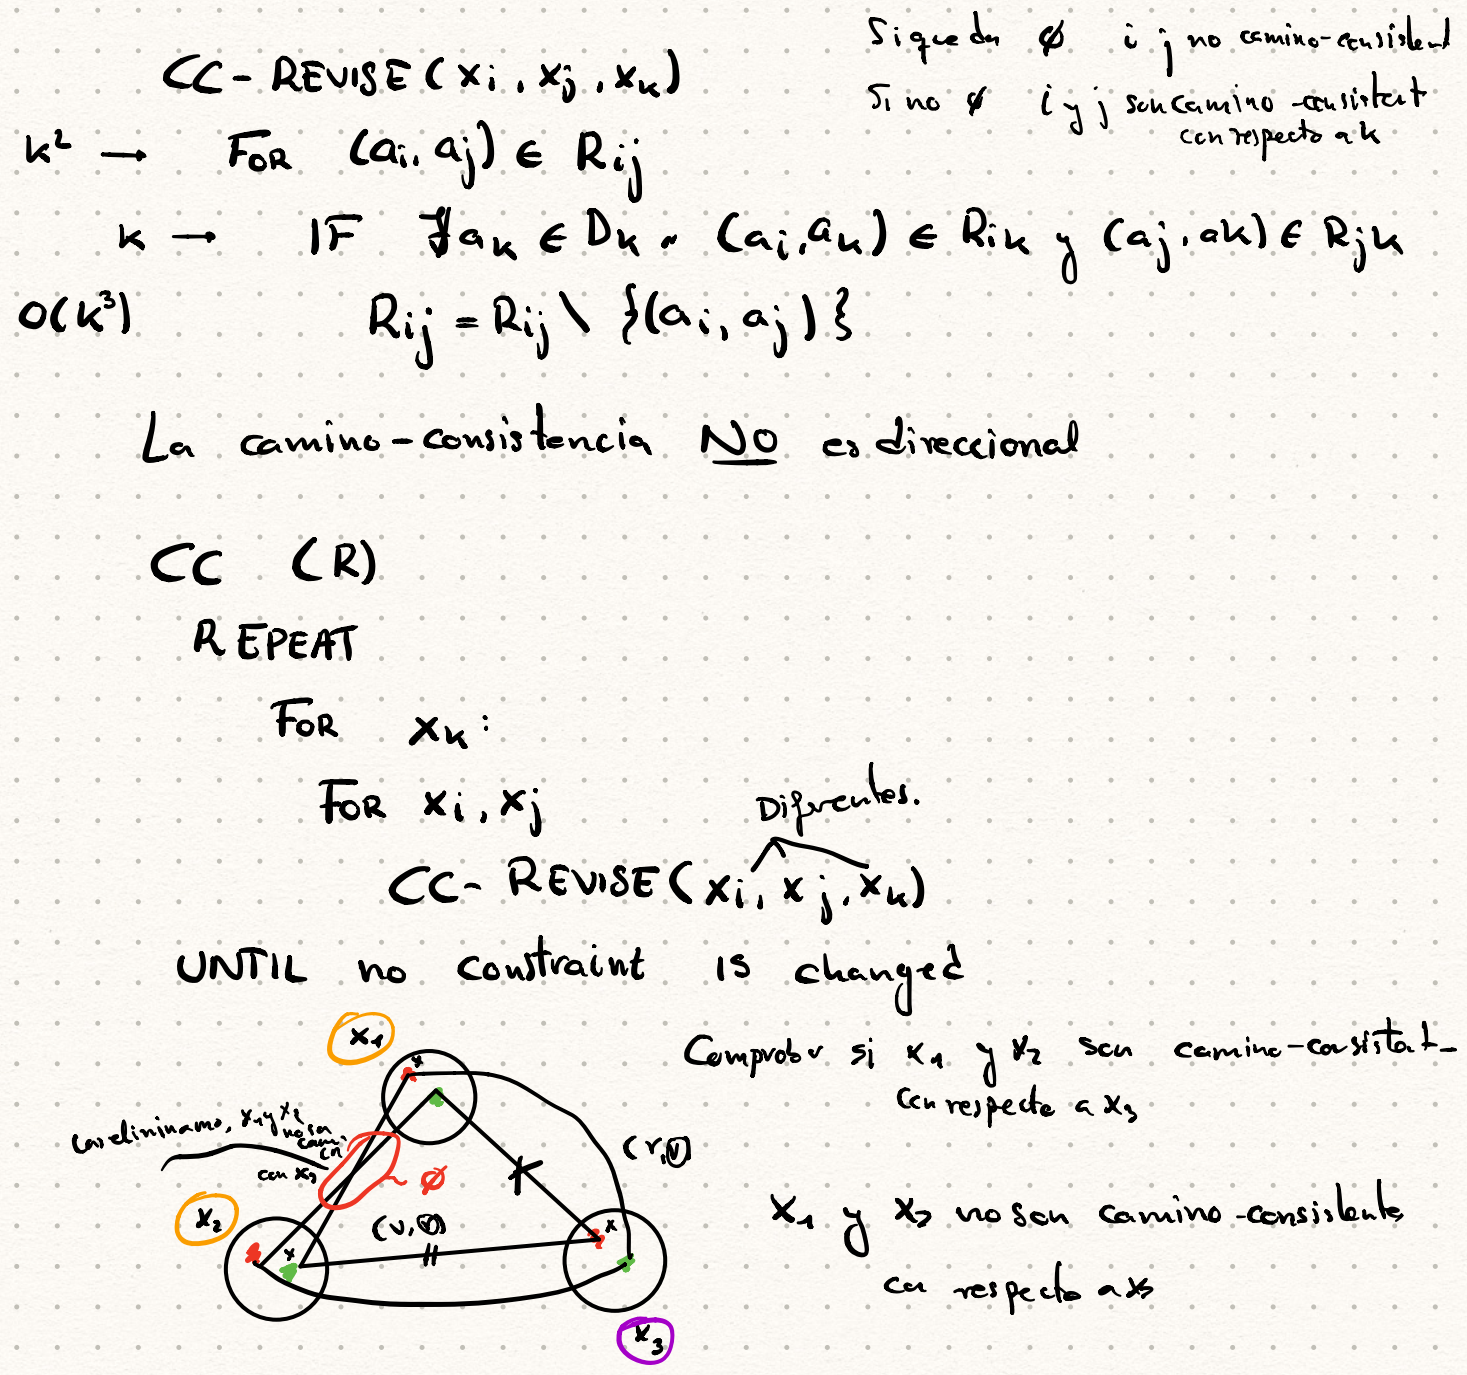
\includegraphics[scale=.15]{Untitled 41.png}}
	\end{figure}
    \end{itemize}

\subsection{Como lo calculamos realmente.}


  Se hace mediante un árbol de búsqueda, como todos los métodos que
  hemos visto hasta ahora.


    Se escoge una variable y se crean tantas ramas como valores tenga el
    dominio de la misma, pero cuando vamos avanzamos por una rama
    calculamos la arco-consistencia con todas las variables anteriores y
    así reducimos el número de ramas que hay que considerar. Además, hay
    que calcular la camino consistencia de todas las variables que
    llevamos y la que estamos contemplando en conjunto.
	\begin{figure}[H]
		\ffigbox[\FBwidth]
		{\caption{C-Co con Árboles}}
		{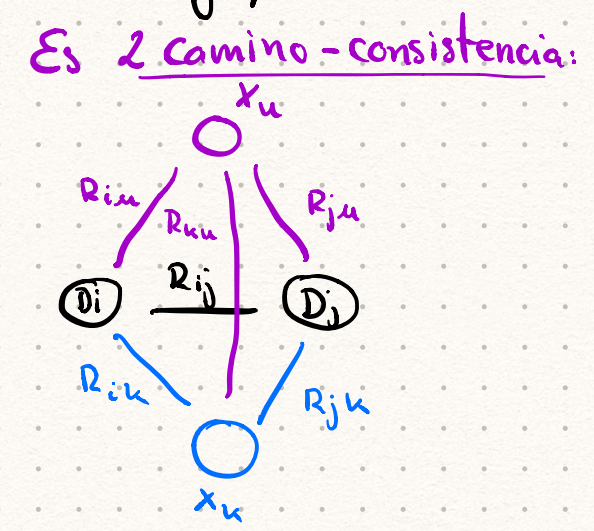
\includegraphics[scale=.23]{Untitled 42.png}}
	\end{figure}    Si llegamos a vacío en algún nodo, tenemos un fallo, y hacemos
    backtracking, si aun así todos salen vacíos no tenemos solución o
    por el contrario si encontramos una no vacía tenemos una
    instanciación global, que cumpla todas las restricciones.

	

\chapter{Tema 4 Búsqueda}

\section{Espacio De Búsqueda}
\begin{figure}[H]
	\ffigbox[\FBwidth]
	{\caption{Espacio De Búsqueda}}
	{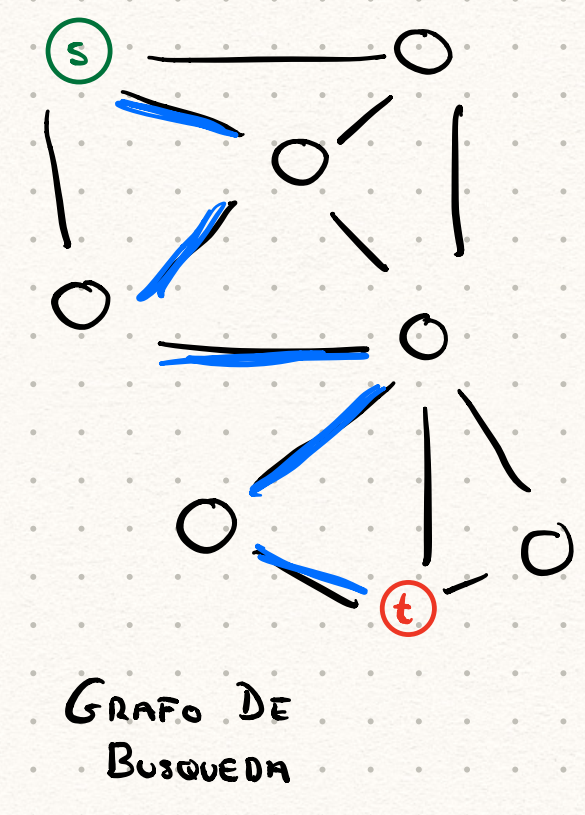
\includegraphics[scale=.25]{Untitled 44.png}}
\end{figure}

  \begin{enumerate}

  \item
    Estados: (estructuras de datos) Contienen la información de tipo
    estático.
  \item
    Operadores: (funciones) Dado un estado nos devuelve los que son
    inmediatamente accesibles.

    \begin{itemize}
  
    \item
      if <precond> then <effects>
    \end{itemize}
  \item
    Un estado inicial, s (start o source).
  \item
    Uno o más estados finales, t (target).

    \begin{itemize}
    \item
      En satisfabilidad conocemos las propiedades del estado final, pero
      no lo conocemos explícitamente. Lo que buscamos es saber cuál es.
    \item
      En optimización se da explícitamente la meta. Lo que buscamos es
      saber cómo llegar a él.
    \item
      Los grafos de búsqueda se recorren con Arboles De Búsqueda.
    \item
      Si sabemos mucho de algoritmos de búsqueda, podríamos resolver
      cualquier tarea de optimización y decibilidad, incluso si es
      exponencialmente difícil.
    \end{itemize}
  \item
    Factor de ramificación (b): número medio de sucesores de cada nodo.
  \item
    Profundidad: número mínimo de niveles hasta alguna solución.
  \end{enumerate}

\section{Algoritmos de Fuerza Bruta (Búsqueda no informada)}
\subsection{Costes unitarios}

  \begin{enumerate}
  \item
    Algoritmo general: (Paso 1. y 3. son operaciones atómicas, pero el
    2. no)

    \begin{enumerate}
  
    \item
      Generar el estado inicial (s).
    \item
      Expandir el primer nodo de la lista abierta.
    \item
      Si alguno de los sucesores es un nodo final, entonces halt

      \begin{itemize}
    
      \item
        En otro caso, ir a 2.
      \end{itemize}
    \end{enumerate}
  \item
    Generar: Es el proceso de creación de un estado en memoria.

    Expandir: Es el proceso de generar todos los sucesores de un nodo.
  \item
    Completitud: Si un algoritmo garantiza que encontrará una solución.

    Admisibilidad: Si un algoritmo garantiza que encontrará una solución
    óptima. No hay una solución más óptima que otra, depende de lo que
    se evalúe.
  \item
    En general, se asume que no hay preferencia en la aplicación de
    operaciones (costes unitarios, si no son iguales son costes
    arbitrarios).
  \end{enumerate}
\subsection{Primero en Amplitud}

  ``Nunca expande un nodo a profundidad d si no ha expandido todos los
  nodos a profundidad (d-1)''

  \begin{figure}[H]
	\ffigbox[\FBwidth]
	{\caption{Primero en Amplitud}}
	{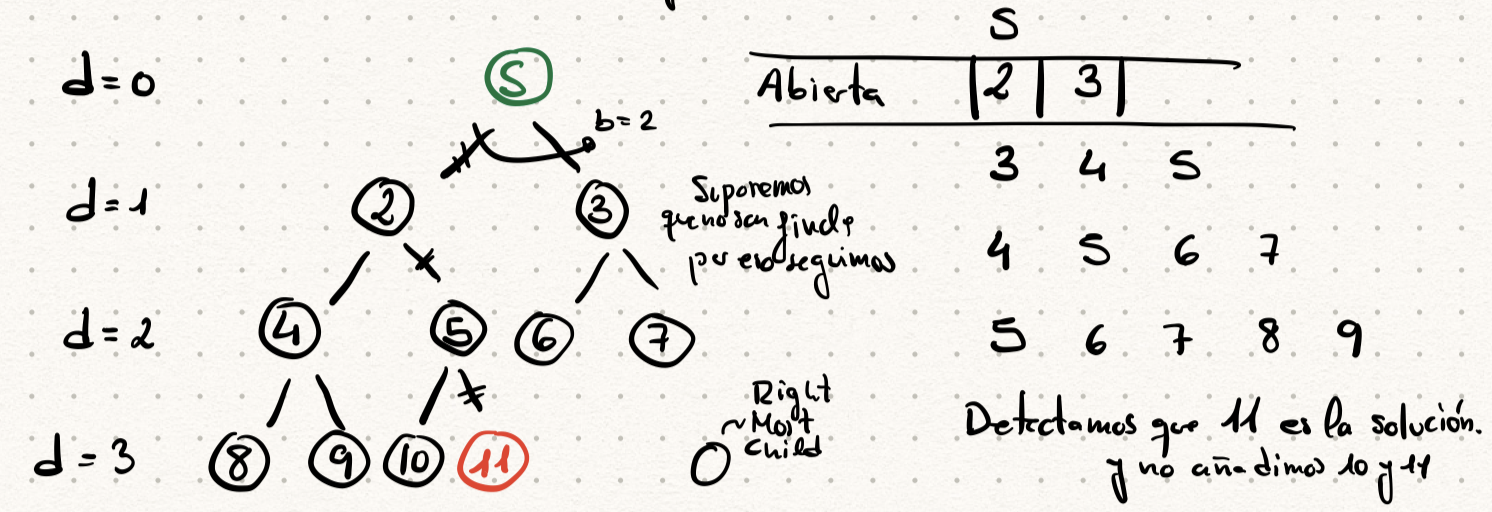
\includegraphics[scale=.25]{Untitled 46.png}}
\end{figure}

	Al ser un problema de satisfabilidad solo nos interesa saber cuál es
    el nodo final, no como llegamos a el. En optimización devuelve el
    camino.

	La lista abierta se implementa con una COLA.

	Es COMPLETO y ADMISIBLE.

	Tiempo: Depende del número de expansiones \(O(b^d)\)

	Memoria: \(O(b^d)\)

	El hecho que de que ambos sean exponenciales es bastante
    desafortunado.

\subsection{Primero en Profundidad}

  ``Se expande el primero de los nodos recién generados hasta que se
  encuentra una solución o se ha alcanzado un \(d_{max}\)''

  
    Se usa una profundidad máxima para evitar caer en una rama infinita
    que nos aleja de la solución.
	\begin{figure}[H]
		\ffigbox[\FBwidth]
		{\caption{Escala Primero en Profundidad}}
		{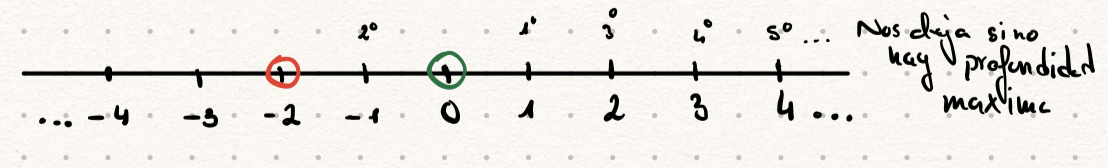
\includegraphics[scale=.25]{Untitled 47.png}}
	\end{figure}
	\begin{figure}[H]
		\ffigbox[\FBwidth]
		{\caption{Primero en Profundidad}}
		{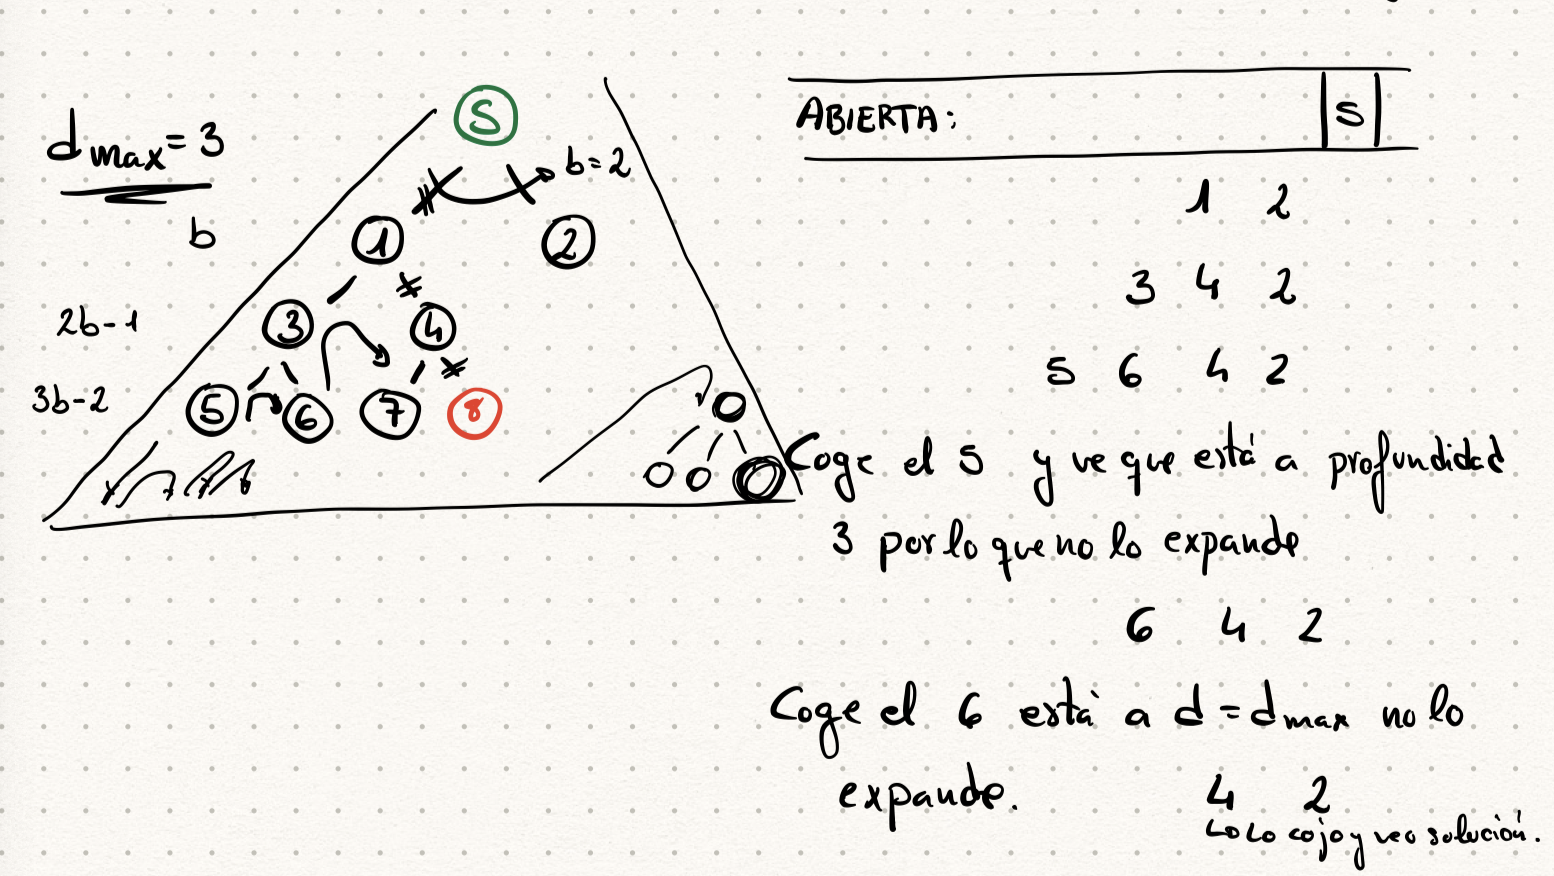
\includegraphics[scale=.2]{Untitled 48.png}}
	\end{figure}
 
	


	Implementa Backtracking con una PILA.

	Completo: No, puede entrar en un bucle.

	Admisible: No, si no es completo no cumplirá el encontrar la óptima.

	Tiempo: \(O(b^d)\)

	Memoria: \(O(d)\) Si solo se almacena 1 sucesor, que lo expandirás
    cada vez y si se hace backtracking ya se generará. Si se almacenan
    todos \(O(bd)\)
  
    Se usa sobre el de amplitud, nos comprometemos hacia una dirección y
    esperamos encontrar la solución.

	
\subsection{Profundidad Iterativa - Iterative Deepening}

  ``Consiste en una serie de exploraciones en profundidad donde
  \(d_{max}\) se incrementa en k en cada iteración''
  \begin{figure}[H]
	\ffigbox[\FBwidth]
	{\caption{Profundidad Iterativa}}
	{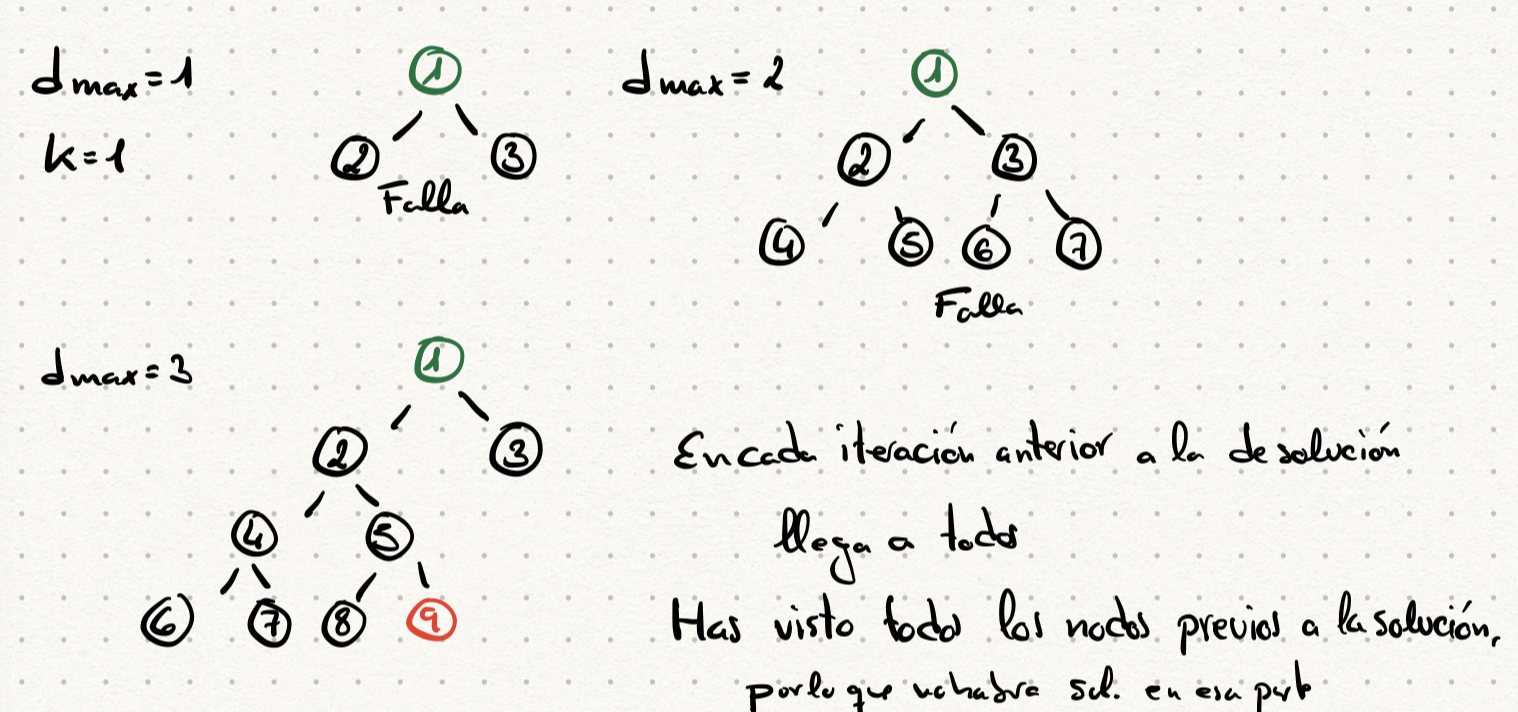
\includegraphics[scale=.3]{Untitled 49.png}}
\end{figure}


    En cada iteración anterior a la solución ha expandido todos los
    nodos.

	Has visto todos los nodos previos a la solución, por lo que habrá
    solución en la otra parte del árbol que todavía no se ha recorrido
    en una iteración.

	Completo: Si. Es como amplitud ve todo.

	Admisible: Si y solo si \(d_{max}=k=1\) Para comprobarlo profundidad
    por profundidad, y no soltarse un posible nivel en el otro lado.

	Memoria: \(O(d)\) Va en profundidad.

	Tiempo: \(\frac {Tiempo (ID)} {Tiempo(BFS)} =\frac {b} {b-1}\)

	Es como hacer primero en amplitud, pero con memoria lineal, que
    compensa que tarde más (aunque no mucho más).

    \begin{itemize}
  
    \item
      \(b^d >> \sum _{i=0}^{d-1} b^i\) (\textgreater\textgreater{} Mucho
      más grande)
    \end{itemize}

	Expandir TODOS los nodos de TODOS los niveles precedentes no es nada
    comparado con lo que se tarda en expandir todos los nodos de una
    nueva profundidad d.

	
\section{Costes arbitrarios}
\subsection{Ramificación y Acotación en Profundidad}


    Definimos el coste de un camino \(\pi<s,n>\) como la suma de los
    costes de los arcos en \(\pi\).

    \begin{itemize}
    \item
      \(g(\pi)= \sum_{i=0}^{k-1} c(n_i,n_{i+1})\) donde
      \(c(n_i,n_{i+1})\) es el coste del arco \(<n_i,n_{i+1}>\) (modelo
      aditivo nosotros lo consideramos siempre, pero en la realidad no
      tiene por qué). Con frecuencia \(g(\pi)\) se representa como
      \(g(n)\).
	  \begin{figure}[H]
		\ffigbox[\FBwidth]
		{\caption{Ramificación y Acotación}}
		{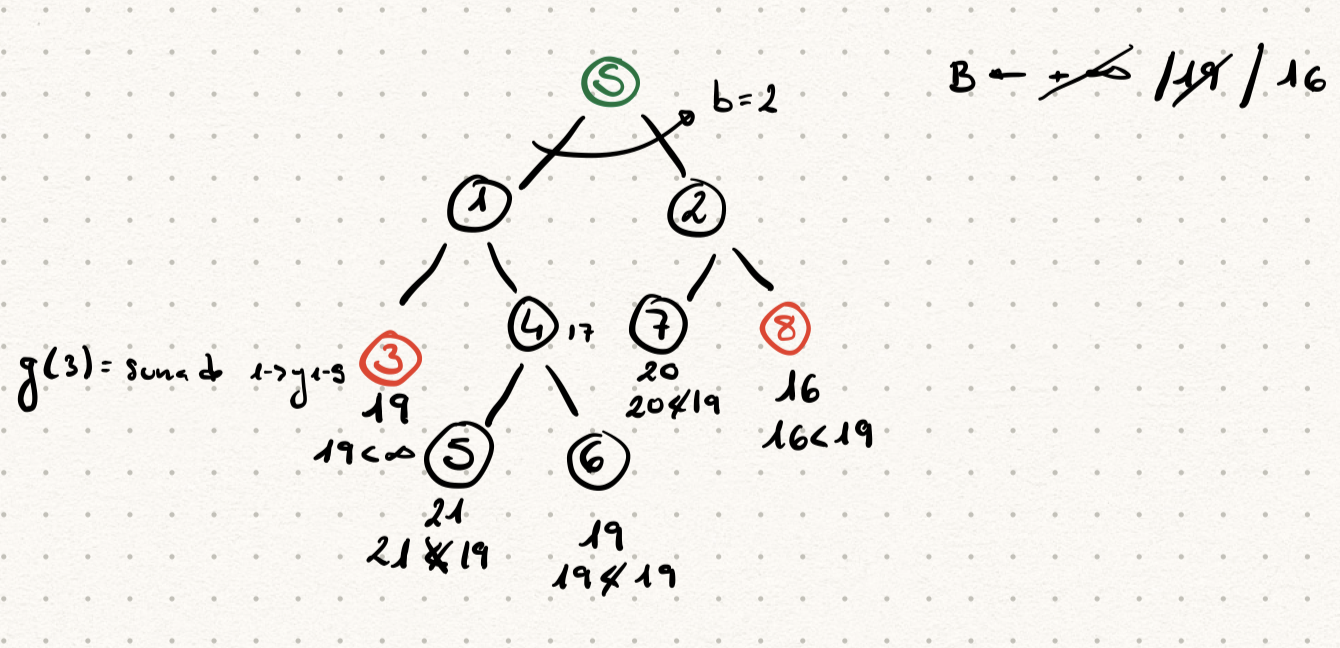
\includegraphics[scale=.3]{Untitled 51.png}}
	\end{figure}
    \end{itemize}

	Seudocódigo (B, valor arbitrariamente grande)

    \begin{enumerate}
    \def\labelenumi{\arabic{enumi}.}
  
    \item
      Generar el estado inicial, s.
    \item
      Coger el primer nodo de Abierta (pila), n.
    \item
      Si n=t entonces B ←\(g(n)\). Salir (hacer backtracking)
    \item
      Expandir \(n: n_1, n_2, ..., n_k\)
    \item
      Si \(g(n_i)<B\), insertar \(n_i\) en abierta,
      \(\forall _i=1,..., k\)
    \item
      Volver a 2.
    \end{enumerate}

    \begin{itemize}
  
    \item
      Costes de \(g(\pi)\): \(g(\pi)\) es monótono creciente. Los costes
      de los arcos son positivos \(c(n_i,n_{i+1}) \geq 0\).
    \end{itemize}

	
\section{Heurísticas}

  \begin{enumerate}
  \def\labelenumi{\arabic{enumi}.}
  \item
    Si no tenemos conocimiento → Búsqueda no informada.

    Si tenemos información perfecta → no hay búsqueda.
  \item
    \(h(n,t)\): Devolver una estimación del coste del mejor camino para
    llegar desde n a t.
  \item
    Sí \(h(n,t) \leq h^*(n,t)\) entonces h es ADMISIBLE.

    El nodo terminal debe tener heurística 0.
  \end{enumerate}

\subsection{Relajación de restricciones (Judea Pearl, 1983)}



    Las restricciones las encontramos en la definición de las
    precondiciones de las operaciones.

	Se observan las precondiciones y vemos cual podemos relajar, una vez
    relajada hallamos algunas soluciones con esta condición y nos damos
    cuenta de cuál es la función heurística en este caso.

	Si \(h_1(n)\geq h_2(n) \forall n\) y ambas son admisibles, entonces
    \(h_1(n)\) está más informada que \(h_2(n)\).

    Preferimos las más informadas.

	Si relajamos todas las restricciones se llama Heurística no
    informada.

	Típicas heurística al relajar restricciones:

    \begin{itemize}
  
    \item
      Casillas mal dispuestas: Número de casillas que no ocupan la
      posición del estado final.
    \item
      Distancia de Manhattan: La suma del valor absoluto de las
      diferencias de las coordenadas.
    \item
      Distancia Euclídea: Hallar la hipotenusa que crea el estado
      actual, el final y un punto a la misma de ambos.
    \end{itemize}
\pagebreak
	Ejemplos:
	\begin{figure}[H]
		\ffigbox[\FBwidth]
		{\caption{Relajación de restricciones I}}
		{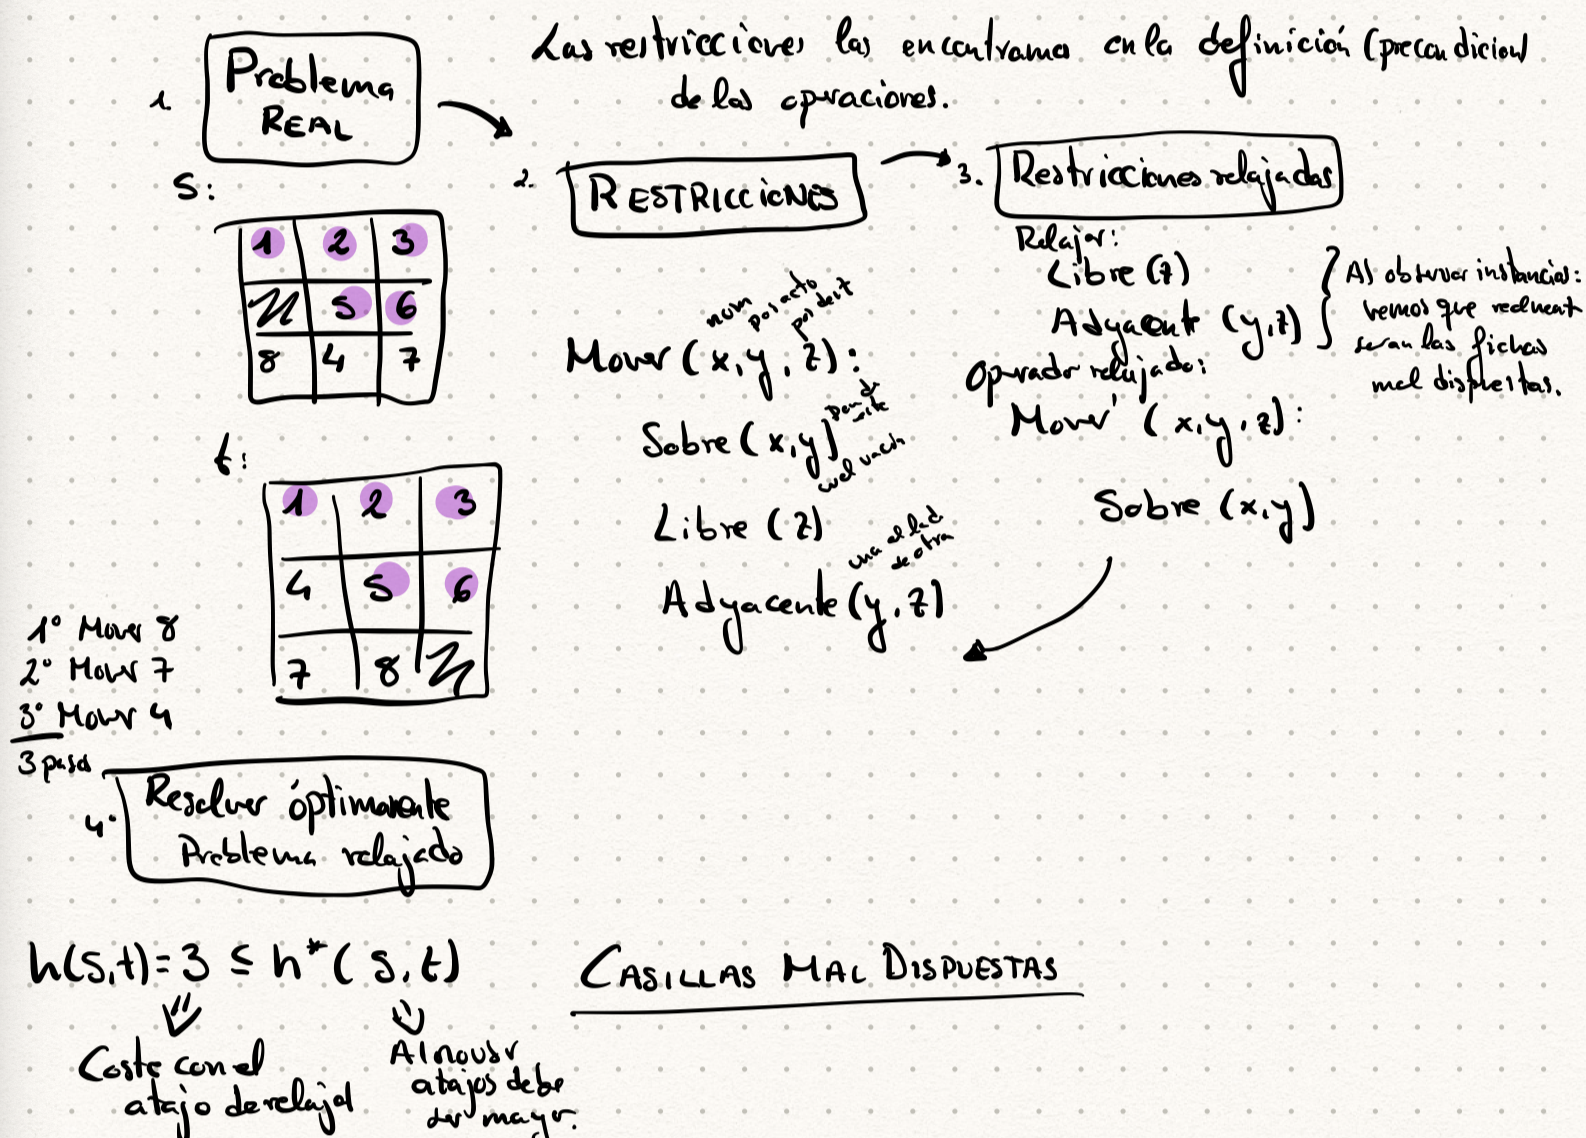
\includegraphics[scale=.22]{Untitled 52.png}}
	\end{figure}
	\begin{figure}[H]
		\ffigbox[\FBwidth]
		{\caption{Relajación de restricciones II}}
		{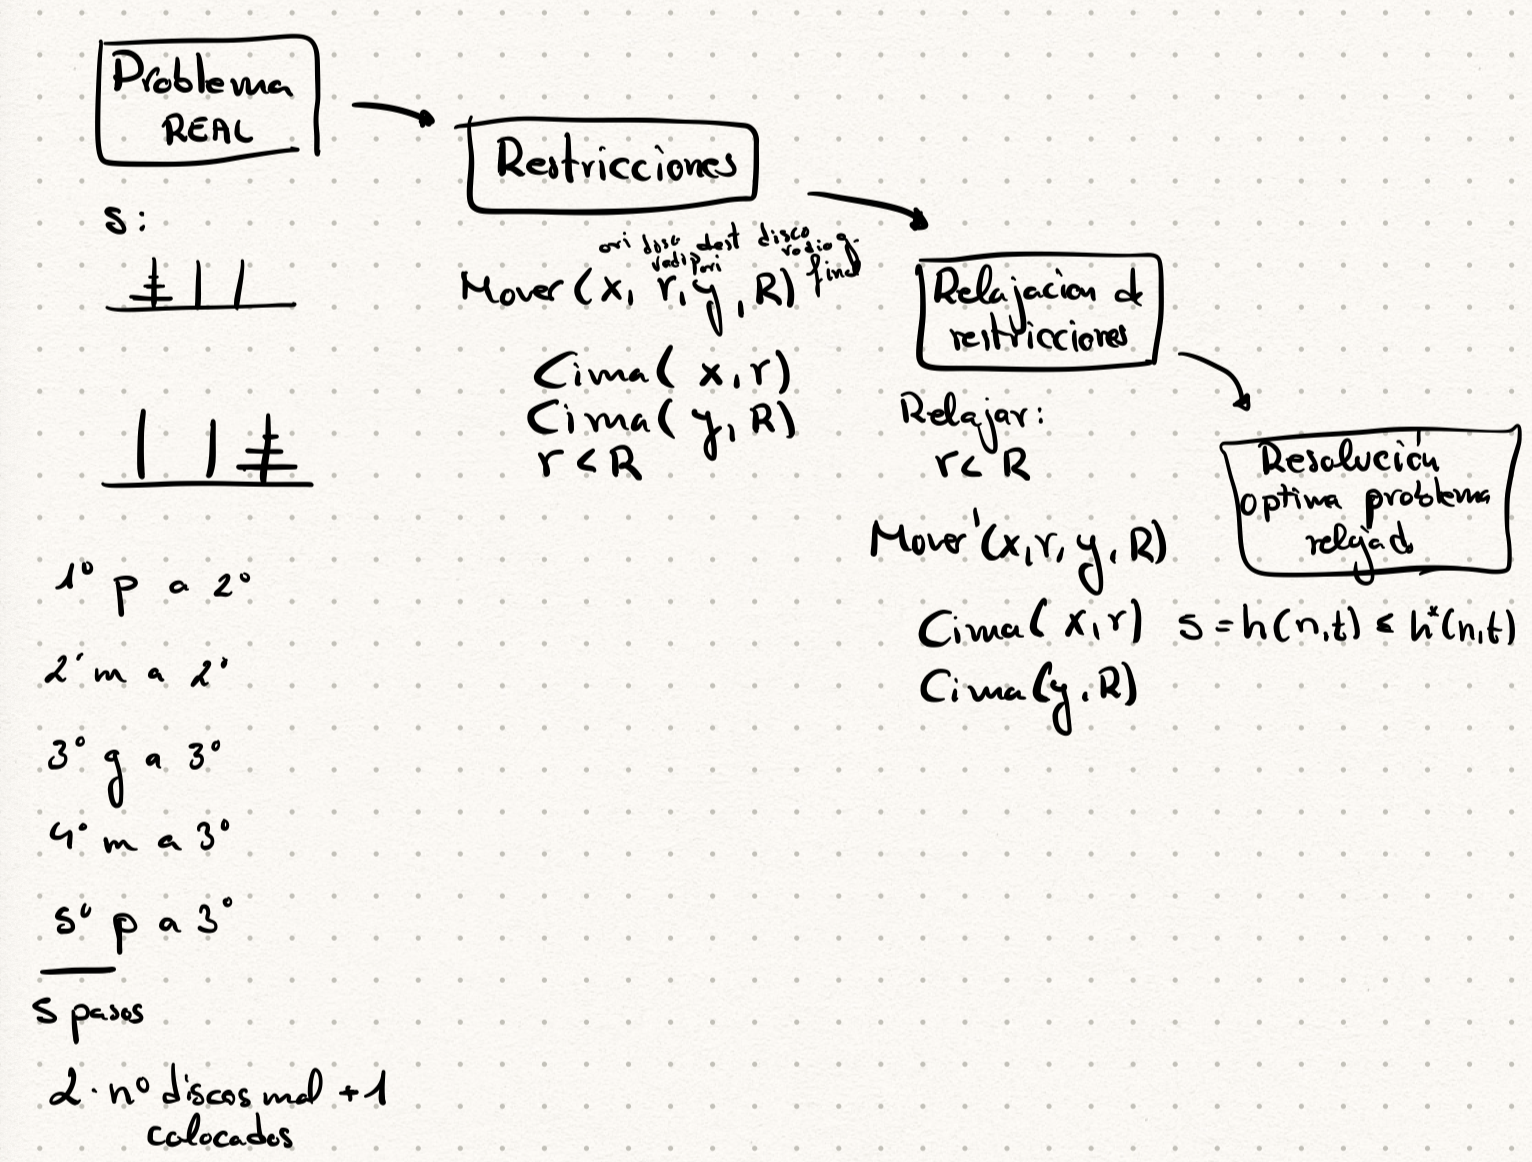
\includegraphics[scale=.22]{Untitled 53.png}}
	\end{figure}
\pagebreak
\section{Algoritmos de Búsqueda Heurística}

  Se aplica tanto a costes unitarios como a costes arbitrarios, pero
  necesitamos emplear 1 heurística.

\subsection{Hill-climbing (De escalada)}

  ``Se escoge para su expansión el sucesor heurísticamente más
  prometedor descartando el resto de sucesores''

  \begin{itemize}

  \item
    Desestima nodos por tener menor coste heurístico.
  \item
    No hay backtracking, al no almacenarse.
  \item
    Aun así, se usa frecuentemente.
  \item
    Completo: no
  \item
    Admisible: no.
  \item
    Memoria: \(O(d)\)
  \end{itemize}

\subsection{Algoritmo de búsqueda en Haz (Beam search)}

  ``Se expanden simultáneamente los k sucesores más prometedores
  heurísticamente''
  \begin{figure}[H]
	\ffigbox[\FBwidth]
	{\caption{Ream search}}
	{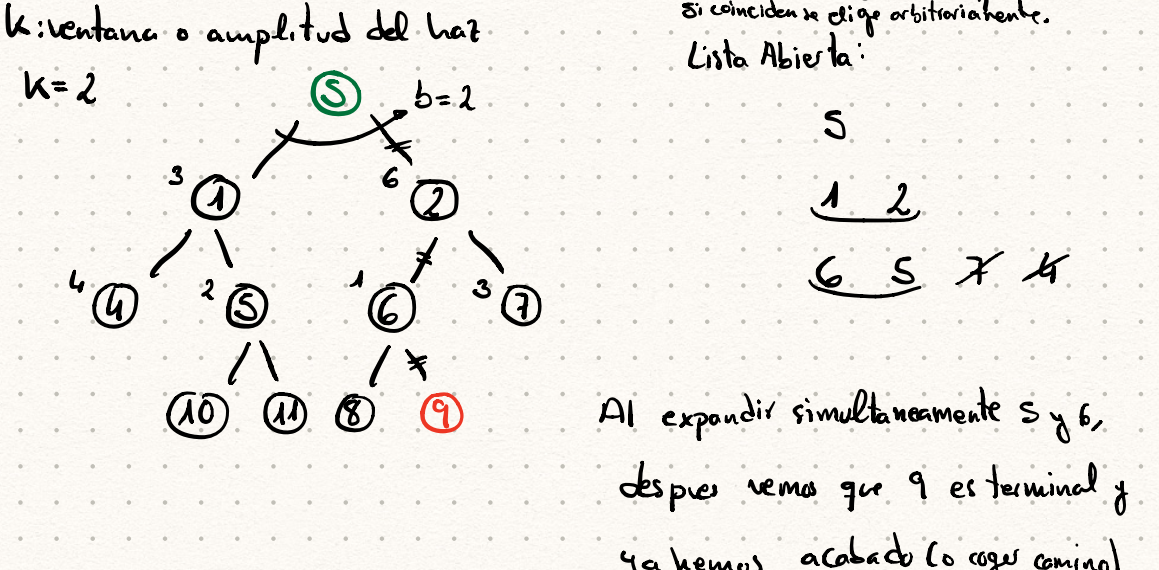
\includegraphics[scale=.22]{Untitled 54.png}}
\end{figure}
 
    k: ventana o amplitud del haz

	Desechamos el resto que no son k. Si coinciden se elige
    arbitrariamente.

	Completo: No, juzga por la heurística.

	Admisibilidad: No , al no ser completo.

	\(BS(k=1)\): Es hill-climbing.

	\(BS(k= \infty)\): Primero en amplitud.

	El k permite decidir la memoria que consume.

	Falta de monotonía de la búsqueda en haz, se obtiene una mejor
    solución con k+1 que k.

	Tiempo: Exponencial.

	Memoria: O(k) lineal, solo almacena los k más prometedores.

	
\subsection{Algoritmo de ``El mejor primero'' (Raphael, Hart, Nilsson, 1968)}
  

  \begin{enumerate}
  \item
    Considerar:

    \begin{enumerate}
  
    \item
      Lista abierta: Contiene todos los nodos generados pendientes de
      ser expandidos, ordena=dos ascendente por f(n)
    \item
      Lista cerrada: Contiene todos los nodos que ya han sido expandidos
      (duplicate detection, evita expandir un nodo expandido
      previamente)
    \item
      Terminación: Procedemos al expandir t, no al generarlo.
    \end{enumerate}
  \item
    Miembros:
	\begin{figure}[H]
		\ffigbox[\FBwidth]
		{\caption{Costes Best first}}
		{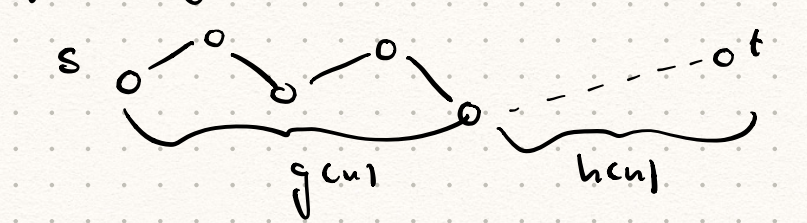
\includegraphics[scale=.45]{Untitled 55.png}}
	\end{figure}
    \begin{itemize}
  
    \item
      \(f(n)=h(n)\) Algoritmo de búsqueda heurística pura.
    \item
      \(f(n)=g(n)\) Dijkstra (Realmente es fuerza bruta)
    \item
      \(f(n) = g(n) + h(n)\) A*
    \end{itemize}
  \item
    Si \(h(n) \leq h^*(n)\) entonces A* es admisible.
  \item
    Tiempo(A*): Exponencial.

    Memoria: Exponencial.

    Especialmente útil por la detección de nodos duplicados.
	\begin{figure}[H]
		\ffigbox[\FBwidth]
		{\caption{Costes Best first}}
		{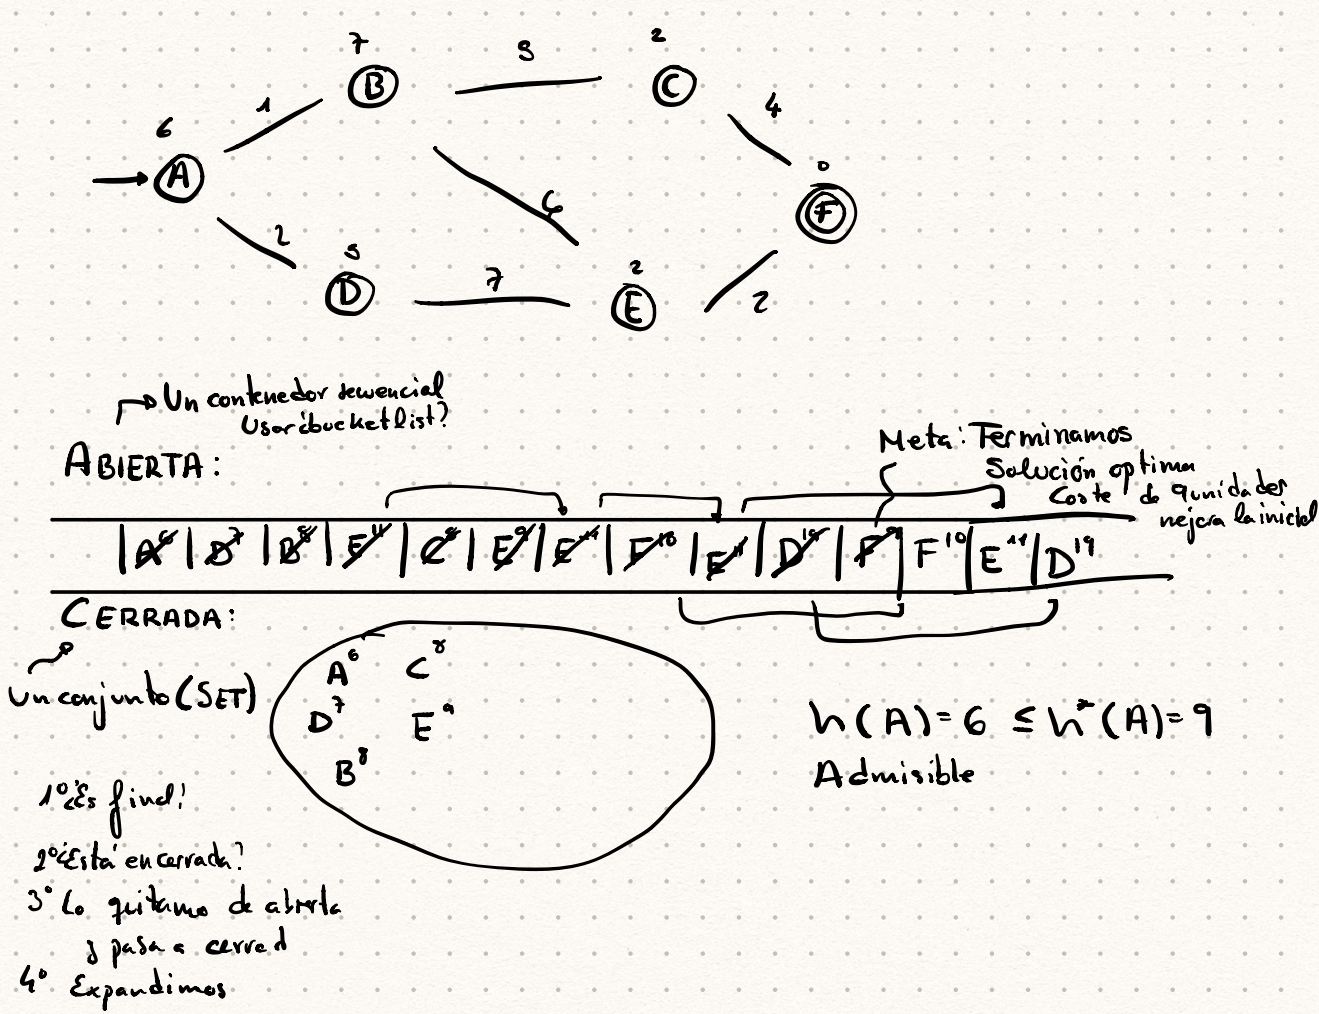
\includegraphics[scale=.32]{Untitled 56.png}}
	\end{figure}
  \end{enumerate}
\pagebreak
\subsection{Iterative-deepening A* - IDA* (Korf, 1985)}

  ``Consiste en una serie de recorridos del \textbf{primero en
  profundidad hasta que \(f(n) > \eta\) o hemos encontrado la solución},
  incrementando f(n) en cada iteración al menor exceso cometido''
  \begin{figure}[H]
	\ffigbox[\FBwidth]
	{\caption{Iterative-deepening A*}}
	{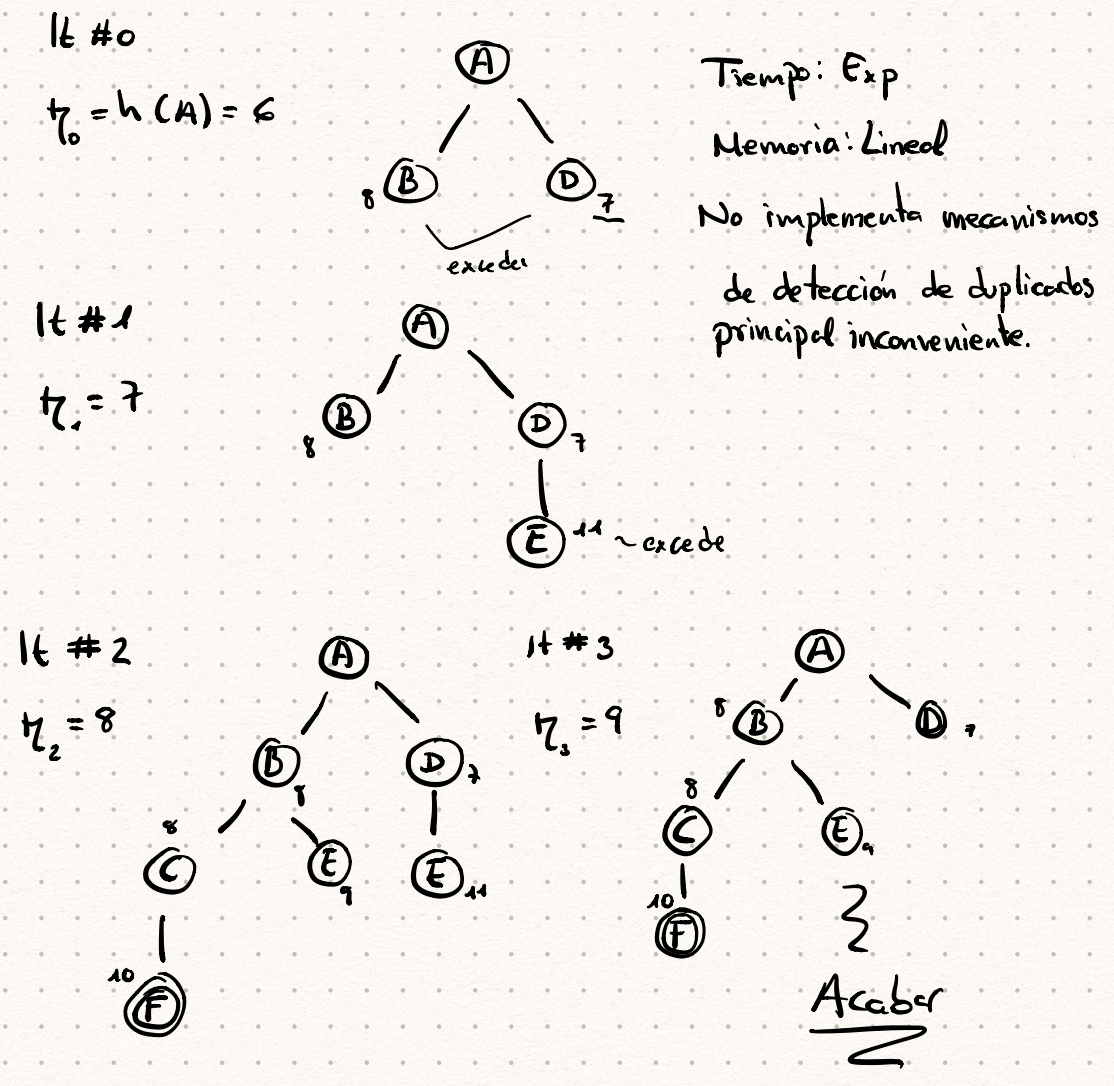
\includegraphics[scale=.38]{Untitled 57.png}}
\end{figure}

\part{Práctica}

\section{Programación Lineal}
  
\includepdf[pages=-]{docs/Presentacin_Problemas_LP.pdf}
  \includepdf[pages=-]{docs/Solucin_Problemas_de_resolucin_grfica.pdf}
  \includepdf[pages=-]{docs/enunciados_representacion_lp.pdf}
  \includepdf[pages=-]{docs/enunciados_simplex.pdf}
  \includepdf[pages=-]{docs/calculo_inversas.pdf}

\section{SAT \& CSP}
  \includepdf[pages=-]{docs/enunciados_sat_csp.pdf}
  \includepdf[pages=-]{docs/soluciones_sat_csp.pdf}

\section{Búsqueda heurística}
  \includepdf[pages=-]{docs/enunciados-espacio-problemas.pdf}
  \includepdf[pages=-]{docs/enunciados-h.pdf}
  \includepdf[pages=-]{docs/enunciados-heuristica.pdf}
  \includepdf[pages=-]{docs/enunciados-no-informada.pdf}
  \includepdf[pages=-]{docs/soluciones-h.pdf}
  \includepdf[pages=-]{docs/soluciones-heuristica.pdf}
  \includepdf[pages=-]{docs/soluciones-no-informada.pdf}
  \includepdf[pages=-]{docs/search.pdf}
  \includepdf[pages=-]{docs/soluciones-espacio-problemas.pdf}

\part{Exámenes}
  \includepdf[pages=-]{docs/hyoene13.pdf}
  \includepdf[pages=-]{docs/hyoene14.pdf}
  \includepdf[pages=-]{docs/hyoene15.pdf}
  \includepdf[pages=-]{docs/hyoene16.pdf}
  \includepdf[pages=-]{docs/hyoene17.pdf}
  \includepdf[pages=-]{docs/hyoene18.pdf}
  \includepdf[pages=-]{docs/hyoene19.pdf}
  \includepdf[pages=-]{docs/hyoene20.pdf}
  \includepdf[pages=-]{docs/hyojul12.pdf}
  \includepdf[pages=-]{docs/hyojun13.pdf}
  \includepdf[pages=-]{docs/hyojun14-es.pdf}
  \includepdf[pages=-]{docs/hyojun15.pdf}
  \includepdf[pages=-]{docs/hyojun16.pdf}
  \includepdf[pages=-]{docs/hyojun17.pdf}
  \includepdf[pages=-]{docs/hyojun18.pdf}
  \includepdf[pages=-]{docs/hyojun19.pdf}
  \includepdf[pages=-]{docs/hyomay12.pdf}

\end{document}